\section{Content Selection Models for Streaming Summarization}

We propose two novel approaches to the streaming summarization task
using biased affinity propagation (AP) clustering \citep{frey2007clustering}
and learning-to-search (L2S) \citep{daume2009search,chang2015learning}.
These models led to the publication of two papers 
\citep{kedzie2015predicting,kedzie2016real}, in addition to participation 
in the TREC Temporal Summarization tracks where we were the top performer in
2014 and the fourth and fifth place performer in 2015 \citep{aslam2015trec,aslam2016trec}. 

In the Temporal Summarization track, the grounding scenario was disaster
summarization, where a participant system received a brief query string 
$\query$ describing a natural or man-made disaster, and the system was 
expected to process a time-ordered stream of documents relevant to the query, 
extracting sentences that were likely to contain important facts about the
event. Each query corresponded to a real-life disaster that was significant
enough to have an associated entry in Wikipedia.

For each query, human annotators also collected a reference set of important 
facts, which we refer to as \textit{nuggets}, 
from the revision history of that query's associated Wikipedia page. 
Nuggets consist of a piece of reference text and timestamp for when this piece
of information first appeared in the Wikipedia revision history. 
See \autoref{fig:eventsnuggets} for example queries and nuggets.

\begin{figure}
    \begin{tabular}{p{7.5cm}|p{7.5cm}}
         \textbf{``hurricane sandy''} &\textbf{``boston marathon bombing''} \\
        \hline
        \parbox{7.4cm}{\small
    $[\textrm{10/23 8:20pm}]$ Sandy strengthened from a tropical depression 
    into a tropical storm \\
    $[\textrm{10/23 8:20pm}]$ 2 pm Oct 23 Sandy moving north-northeast at 4 
    knots \\
    $[\textrm{10/23 8:53pm}]$ forecast track uncertain \\
    $[\textrm{10/25 12:20am}]$ In Jamaica damage was extensive
} & \parbox{7.4cm}{ \small
    $[\textrm{04/15 7:31pm}]$ Authorities are investigating a report of two 
    explosions at the finish line of the race. \\
    $[\textrm{04/15 8:29pm}]$ Some Boston Transit system service has been 
    halted.\\
    $[\textrm{04/16 12:37am}]$ Police confirmed another explosion at the JFK
    Library.
}
\end{tabular}
    \caption{Example event queries in bold, and several example nuggets below.
    Nugget timestamps are show in brackets.}
    \label{fig:eventsnuggets}
\end{figure}




We will refer to the set of extracted sentences as the update or extract
summary interchangeably. Similarly, we will use the phrases extract a sentence,
select a sentence, or emit a sentence to mean we add a sentence in the 
document stream to our rolling update summary. If a sentence $\strsent$ 
expresses the same piece of information as a nugget text $\nugget$ 
we say that $\strsent$ contains $\nugget$ or $\nugget \in \strsent$.

Systems are rewarded when they find sentences that contain important and novel
nuggets. Systems are penalized for 
selecting sentences that are irrelevant (i.e. contain no nuggets) or 
contain nuggets already covered by previous updates. 
Latency penalized metrics are also computed where
the importance of a nugget decays over time. E.g. if a system
recovers the nugget ``25 people were reported injured,'' several days
after this fact was first reported, it will receive less credit for it
than the system that emits that nugget an hour after it enters the 
document stream. See \cite{aslam2014trec} for more details on this decay 
factor. Intuitively, latency penalized metrics capture the idea that stale
information in a rapidly evolving disaster is less useful and possibly
distracting.

Streaming summarization is a very hard task compared to single and 
multi-document summarization. In the latter case, the context for the 
summarization is fixed, and the input documents are usually quite 
topically focused, minimizing the prevalence of completely irrelevant 
information. In fact, in most multi-document evaluation settings, the
document collections were manually created leading to very topically
coherent text collections. 
\cite{baumel2016topic} for example found that the DUC
query focused summarization datasets are so on topic that a summarization
system could completely ignore the query and perform just as well as a
query aware system.

\begin{figure}
\begin{subfigure}{.47\textwidth}
\begin{algorithmic}[1] 
\Procedure{OracleSummarize}{}
  \State $\updates \gets \varnothing$ \Comment{Init. update summary.}
  \State $\hat{\nuggets} \gets \varnothing$ \Comment{Init. found nuggets.}
  \For{$\strsent \in \strsents$} 
    \If{$\exists \nugget$ s.t. $\nugget \in \strsent
            \wedge \nugget \notin \hat{\nuggets}$ }
      \State $\mathcal{U} \gets \mathcal{U} \cup \{\strsent\}$ 
      \State $\hat{\mathcal{N}} \gets \hat{\mathcal{N}} \cup \{\nugget \in \strsent\}$ 
    \EndIf
  \EndFor
  \State \Return $\mathcal{U}$
\EndProcedure
\end{algorithmic}
    \caption{Greedy oracle streaming summarization algorithm.}
    \label{alg:ts_greedy_oracle}
\end{subfigure}
~
\begin{subfigure}{.48\textwidth}
\begin{algorithmic}[1] 

  \Procedure{GenericSummarize}{}
  \State $\mathcal{U} \gets \varnothing$ \Comment{Init. update summary.}
  \For{$\strsent \in \mathcal{S}$} 
    \State $\hat{\salience} \gets \operatorname{salience}(\strsent, \query) $
    \State $\similarity \gets \operatorname{similarity}(\strsent, \updates)$
    \State $\extract \gets \operatorname{decide}(\hat{\salience}, \similarity)$
    \If{$\extract = 1$}
        \State $\updates \gets \updates \cup \{\strsent\}$
    \EndIf
  \EndFor
  \State \Return $\updates$
\EndProcedure
\end{algorithmic}
    \caption{Greedy generic streaming summarization algorithm.}
    \label{alg:ts_greedy_generic}
\end{subfigure}
\caption{Oracle and generic greedy stream summarization algorithms. 
$\mathcal{S}$ is a time-ordered set of sentences from the document stream 
for query $\query$.}
\end{figure}



%?When considering whether or not to select a sentence for the update summary
%?there are two considerations. First we must estimate the salience, or 
%?importance, of the sentence with respect to the query. This is a proxy
%?for assesing whether or not a sentence contains a nugget. 
%?Second, we must consider
%?whether the relative importance of the sentence in the context of previous
%?updates and current candidate updates warrants selecting it for the summary.
%?This is a proxy for determining if the sentence contains any novel nuggets
%?with respect to our current update summary.


If we had clairvoyant knowledge of which nuggets were contained in each
sentence in the document stream,
this task would be trivial in that the greedy algorithm in 
\autoref{alg:ts_greedy_oracle} would return an approximately optimal summary.
Since we do not know this information at test time, we attempt approximate
the if-statement in line 5 of the oracle by answering the following proxy 
questions:
\begin{enumerate}
    \item How salient is sentence $\strsent$ with respect to query $\query$?
    \item How similar is the sentence $\strsent$ with respect to the set of 
            previously selected updates $\hat{\strsent} \in \updates$?
\end{enumerate}
The generic stream summarization algorithm we aim to implement is presented
in \autoref{alg:ts_greedy_generic}.

The two models we propose to solve these more tractable problems come with
different trade-offs. They both, however, rely on a feature-base 
representation of the stream sentences to make salience and selection 
predictions. In the next sub-section, we describe the different feature
groups before describing each of the models used to perform the streaming
summarization task.







%In the next sections, we describe to proposed solutions to this problem.
%Both approaches use feature-based regression models to eestimate sentence
%salience and so we briefly describe the features here.

\begin{figure}
\center
\begin{tabular}{r|ccccc|ccccc}
& \multicolumn{5}{c}{\bfseries Static Features} 
& \multicolumn{5}{c}{\bfseries Dynamic Features} \\
Model
& \rot{90}{1em}{surface}
& \rot{90}{.5em}{query}
& \rot{90}{1em}{lang. mod.} 
& \rot{90}{1em}{nugget likelihood} 
& \rot{90}{1em}{single doc} 
& \rot{90}{1em}{geographic relevance}
& \rot{90}{1em}{temporal relevance}
& \rot{90}{1em}{document frequency}
& \rot{90}{.5em}{stream language models}
& \rot{90}{.1em}{update similarity} \\
\hline
Salience biased AP & X & X & X &   &   & X & X &   &   &   \\
Learning-to-Search & X & X & X & X & X &   & X & X & X & X \\
\end{tabular}
\caption{Feature groups used by each model.}
\label{fig:strfeats}
\end{figure}




\subsection{Features for Sentence Importance Estimation}

The streaming summarization problem is difficult precisely because the context
is constantly shifting. We cannot rely solely on word frequency because
the counts of particular ngrams will be shifting throughout the period of 
interest. Instead we compute several groups of sentence features that are
specifically helpful for the query focused task. We divide our features
into two groups: static and dynamic features. Static features do not take into
account previous sentence selection decisions, while dynamic features
can be used information about current state of the update summary or stream
behaviour. \autoref{fig:strfeats} shows which feature groups were used 
in each of our two approaches. In general, incorporating dynamic features
into the learning-to-search approach is much easier.


\subsubsection{Static Features}
\paragraph{Simple Surface Features} 

The document stream that we will be operating over is incredibly noisy,
full of automatically extracted article text from raw web pages in 
dramatically different formatting. As a result, the underlying text is often
full of wep page headers, headlines to other stories, and irrelevant link text.We this group of basic features to help identify typical content bearing
sentences in the AP news style \citep{ap_style_guide}. These features 
include sentence length, the average number of capitalized words,
document position, sentence length in words, and the average number of 
named entities. Length and position features have been used previously in
other learning based models of sentence salience
\citep{kupiec1995trainable,conroy2001using}.

\paragraph{Query Features} To ensure the focus of the update summaries,
we employ query match features that count frequency of query term matches
in the sentence. We also do a simple query expansion using WordNet 
\citep{miller1995wordnet}
to find  synonyms, hypernyms, and hyponyms for the query event type and compute
a similar term match count with the expansion.
Queries in the Temporal Summarization data are also labeled with even type.
See \autoref{fig:eventtypes} for the list of query event types we used. 
For the \emph{earthquake} query type, for example, we find the following terms:
``quake'', ``temblor'', ``seism'', and ``aftershock''.


\begin{table}
\begin{tabular}{r | l}
\textbf{Event Type} & \textbf{Event Queries} \\
\hline
Storm & hurricane isaac, hurricane sandy, midwest derecho, typhoon bopha\\
Earthquake & guatemala earthquake  \\
Meteor Impact & russia meteor \\
Accident & buenos aires train crash,  pakistan factory fire\\
Riot & egyptian riots\\
Protest & bulgarian protests, egyptian protests \\
Hostages & in amenas hostage crisis \\
Shooting & colorado shooting, sikh temple shooting\\
Bombing & boston marathon bombing, hyderabad explosion \\
Conflict & konna battle \\
\end{tabular}
\caption{TREC Temporal Summarization query event types with example queries.} 
\label{fig:eventtypes}
\end{table}

\paragraph{Language Model Scores}

We rely on a pair of language models to assess the likelihood of observing
a given sentence in the document stream. The first language model is 
intended to be a generic news model, trained on New York Times and 
Associated Press sections of the Gigaword corpus \citep{graff2003english}. 
This model serves a similar purpose as the simple surface features in helping
to identify newswire-like sentences that are likely to contain informative
content.
The second model is query type specific and intended to focus the summarizer
on sentences from the same domain of the query. For each query type, we 
constructed an in-domain corpus of Wikipedia news articles belonging to
categories and pages related to the event type. The corpus is 
semi-automatically constructed: first a set of high-level categories are 
selected and then all pages belonging to those initial categories or
any sub-categories are automatically added. 
For example, the language
model for the event type ``earthquake'' is estimated
from Wikipedia pages under the category Category:Earthquakes.
For the actual summarization system features, we use the average token log
likelihood under each model as a feature.
We use the SRILM toolkit \citep{stolke2002srilm} to implement a 5-gram 
Kneser-Ney model \citep{kneser1995improved} for both the general and type
specific language models. 

\paragraph{Nugget Likelihood}
Using human judgements from 2014 Temporal Summarization we were able to obtain
example sentences that contained many of the nuggets in our corpus. We used
these judgements to train an ngram based classifier to predict a binary 
label $y$ for a sentence, with $y=1$ if it contained any event nugget and
$0$ otherwise. We used the probability of $y=1$ as an additional feature.

\paragraph{Single Document Summarization Features}
We used several unsupervised sentence ranking methods from the single 
document summarization literature to get several sentence rank features.
Inspired be the \textsc{SumBasic} summarizer \citep{nenkova2005impact}, we
compute the average and sum of unigram probability of each sentence using 
sentence's document unigram distribution. Inpsired by \citep{guo2013updating},
for each sentence we compute the average cosine distance to the remaining 
sentences in it's enclosing document. Finally, we compute the document
level centroid rank \citep{radev2000centroid} and LexRank 
\citep{erkan2004lexrank} for each sentence.

\subsubsection{Dynamic Features}
\paragraph{Geographic Relevance} 
The queries in the Temporal Summarization data are all grounded to physical
events in the world and we would like to exploit that. For example, while
there are sadly many reports of bombings or explosions at any given time 
around the world, when summarizing the query ``boston marathon bombing'' 
we are only really interested in news from a relatively proscribed 
geographic area, in this case, Boston, Massachusets. Implementing 
a geographic relevance signal is quite difficult in practice since 
we do not have ground truth location data for each event query, and some
events like hurricanes can be on the move. We opt instead to extract all
location mentions (using a named entity tagger) and get the lattitude
and longitude coordinates
of each mention using the Bing maps API \citep{bingmaps}. Location
mentions within the same hour are clustered, and the cluster centers are 
used as the canonical event locations for the query at that time. 
To get features for each sentence in the stream, we find the location of
the news article it came from and then compute average distance of the 
article to the query event locations.


%?The disasters
%?in our corpus are all phenomena that affect some
%?part of the world. Where possible, we would like
%?to capture a sentence’s proximity to the event, i.e.
%?when a sentence references a location, it should be
%?close to the area of the disaster.
%?There are two challenges to using geographic
%?features. First, we do not know where the event is,
%?and second, most sentences do not contain references
%?to a location. We address the first issue by
%?extracting all locations from documents relevant to
%?the event at the current hour and looking up their
%?latitude and longitude using a publicly available
%?geo-location service. Since the documents that are
%?at least somewhat relevant to the event, we assume
%?in aggregate the locations should give us a rough
%?area of interest. The locations are clustered and
%?we treat the resulting cluster centers as the event
%?locations for the current time.
%?The second issue arises from the fact that the
%?majority of sentences in our data do not contain
%?explicit references to locations, i.e. a sequence of
%?tokens tagged as location named entities. Our intuition
%?is that geographic relevance is important in
%?the disaster domain, and we would like to take ad


\paragraph{Temporal Relevance} As we track a query over time, the document
stream will ebb and flow as the underlying event unfolds. With hurricanes
for example, forecasters are usually watching a tropical storm as it grows
and predicitng where it might make landfall. As a result, news about a major
hurricane grows gradually, peaking after its main contact with land
and gradually diminishing. An eartquake on the otherhand gives no warning,
and there is a sudden spike in the query relevant document stream.
While we do not
do an extensive study of different event type shapes (which would certainly 
be very interesting), we would like to take advantage of spiking or bursty
activity in the docuemnt stream as a signal for our summarization system.
We do this by maintaining IDF values for each hour of the document stream.
We create 24 average TF-IDF features for each sentence as if it had occurred
in each of the previous 24 hours; large changes in any of the individual
features should be representative of a spike in the news.

\paragraph{Document Frequency} We also compute the hour-to-hour
percent change in document frequency of the stream. This
feature helps gauge breaking developments in an unfolding
event. As this feature is also heavily affected by the daily
news cycle (larger average document frequencies in the morning
and evening) we compute the 0-mean/unit-variance of this
feature using the training streams to find the mean and variance
for each hour of the day.



\paragraph{Stream Language Models}
We construct several simple unigram language models that we update with 
each new document that we see in the stream. Using these models 
we compute the sum, average, and maximum token likelihood
of the non-stop words
in the sentence. We compute similar quantities restricted to
the person, location, and organization named entities.

\paragraph{Update Similarity} The average and maximum cosine similarity
of the current sentence to all previous updates is computed
under both the tf-idf bag-of-words and latent vector
representation. We also include indicator features for when
the set of updates is empty (i.e. at the beginning of a run) and
when either similarity is 0.


\subsection{Model 1: Salience Biased Affinity Propagation Clustering}

  \begin{figure}
\begin{algorithmic}[1] 
\Procedure{APSalienceSummarize}{}
  \State $\updates \gets \varnothing$ \Comment{Init. update summary.}
  \For{$\strsents_t \in \strsents$} 
    \State $\hat{\Salience} \gets \operatorname{salience}(\strsents_t, \query)$
        \Comment{Estimate sentence salience for each 
                 $\strsent \in \strsents_t$.}
    \State $\Similarity \gets \operatorname{similarity}(
           \strsents_t, \strsents_t)$ \Comment{Compute similarity 
           between each $\strsent_i, \strsent_j \in \strsents_t$.}
    \State $\exemplars \gets \operatorname{AffinityPropagation}(\hat{\Salience}, \Similarity)$ \Comment{Get exemplar sentences $\exemplars$ with AP.}

    \For{$\strsent \in \exemplars$}
      \If{$\hat{\Salience}_\strsent > \lambda_1 \wedge \max \operatorname{similarity}(\updates, \strsent) > \lambda_2$}
        \State $\updates \gets \updates \cup \{\strsent\}$
      \EndIf
    \EndFor
%    \If{$\exists \nugget$ s.t. $\nugget \in \strsent
%            \wedge \nugget \notin \hat{\nuggets}$ }
%      \State $\mathcal{U} \gets \mathcal{U} \cup \{\strsent\}$ 
%      \State $\hat{\mathcal{N}} \gets \hat{\mathcal{N}} \cup \{\nugget \in \strsent\}$ 
%    \EndIf
  \EndFor
  \State \Return $\mathcal{U}$
\EndProcedure
\end{algorithmic}
    \caption{Salience-biased AP clustering based streaming summarization 
             algorithm.}
    \label{alg:ts_sap_algo}
\end{figure}




  Identifying potential updates from the document stream is hard in part
  because we may not have enough context to use word frequencies as a 
  reliable proxy for salience. Our first proposed method accounts for this
  in two ways. 

  First, we process the stream in hourly batches, i.e. we collect all the
  sentences from the last hour and then decide which sentences if any to
  add to the update summary. The trade-off we make is that fast breaking
  events may not immediately be covered by the summarizer.

  Second, we use an exemplar-based clustering algorithm,
  called Affinity Propagation (AP) \citep{frey2007clustering}, that combines
  sentence level salience predictions with pairwise sentence similarities
  to identify a set of exemplar sentences that would make for good 
  additions to the updates summary. The pairwise similarity factors work 
  as our replacement for the ngram-frequency based signal we would normally 
  use in traditional MDS; a sentence that has high overall similarity to
  the other sentences in the batch is likely to be an exemplar and
  more so if it's salience prediction is high relative to the batch.

  Finally, given a set of exemplar sentences $\exemplars$, we add those
  whose maximum similarity to a previous update is below a threshold.
  The final algorithm is presented in \autoref{alg:ts_sap_algo}.



  We describe our process for computing salience and similarity in
 the next sections, before describing the AP clustering algorithm.



%?  We next describe the 
%?
%?
%?
%?  In this model, we process the document stream in hourly batches, 
%?  first predicting the salience of the individual sentences and then 
%?  using affinity propagation (AP) to select a set of exemplar sentences.
%?  Exemplar sentences that have predicted salience above a threshold 
%?  and are below a similarity threshold to previously select sentences are
%?  then emitted to the user as an update summary.





  \subsubsection{Salience Estimation}

  Given a sentence $\strsent \in \strsents$ we would like to predict it's 
  salience with respect to a query $\query$. When we were developing this 
  model,
  we did not have access to many human judgements of query or nugget relevance,
  and so we relied on an automatic measure of sentence salience computable
 from the nugget data we had.

Given a query $\query$, sentence text $\strsent$, and query's nugget texts 
$\nugget \in \mathcal{N}(q)$, we define
the sentence salience $\salience$ as
\[ \salience = \max_{\nugget \in  \nuggets(\query)} \operatorname{similarity}(\strsent, \nugget)\]
where $\operatorname{similarity}(\cdot, \cdot)$ is the cosine similarity of a
low-dimensional representation of the sentence and nugget text.
We used the weighted matrix factorization method of \cite{guo2012simple}
which projects a text's sparse high-dimensional bag-of-words representation
into a dense, low-dimensional vector. We use this method to compute 
sentence similarity in the AP clustering algorithm.


%  Given the feature representation of a sentence, we want to predict how
%confident we are that it contains one or more nuggets. While we have
%many sentences in our corpus, we did not have may sentence level judgements
%about the nuggets that they contained. 
%Lacking these gold annotations, we instead get noisy salience annotations 
%using the maximum similarity of the nugget texts to the sentence texts.
%Formally, given a query $q$, sentence text $s$, and query's nugget texts $n \in \mathcal{N}(q)$
%the sentence salience $y$ is 
%using the following equation:
%\[ y = \max_{n \in  \mathcal{N}(q)} \operatorname{sim}(s, n)\]
%where $\operatorname{sim}$ is a semantic similarity measure (in practice
%we used the weight matrix factorization method of \cite{wmtf}).

We use a Gaussian process-based regression model \citep{rasmussen2004gaussian}
to predict $\salience$ from a feature representation $\phi(\strsent)$ 
\emph{without} knowledge of the nuggets. See \autoref{fig:strfeats}
for the list of feature groups used in the salience regressor.
We use seperate radial basis function (RBF) kernels for each 
feature group, and use the sum of all the kernels as final
kernel matrix for fitting the model.
We fit a separate regressor for each query in our dataset using 1000
randomly sampled sentences from each query's associated relevant document 
stream. At prediction time for a specific query, we hold out that query's salience
model, and use the average prediction of the remaining models to obtain
a salience estimate $\hat{\salience}$ for sentences in the stream.

\subsubsection{Sentence Selection with Salience-biased Affinity Propagation Clustering}


    AP clustering is a factor-graph based clustering
    method that simultaneously selects exemplar data points and maps 
    the remaining data points to one of the exemplars \cite{frey2007clustering}. 
    The exemplar mappings determine the clusters.
    AP has a number of nice properties for extractive summarization.
    First, as an exemplar based clustering method, the cluser center
    is guarantee to be an actual data point observed in the input; 
    this removes the added step of selecting a representative sentence
    if we had used for $k$-means clustering, for example.
    Two, the number of clusters that result is adaptive and 
    based on the interaction of the unary and pairwise factors.

    Given a set of $d$ datapoints $\mathcal{X} = \{x_1, \ldots, x_d\}$, 
    AP finds a set of
    exemplar datapoints $\exemplars \subset \mathcal{X}$ and a mapping
    $A : \mathcal{X} \setminus \exemplars\rightarrow\exemplars$ of the 
    remaining points to one of the exemplars. The configuration of exemplars
    and exemplar assignments is represented as a factor graph, where the
    objective function expresses a net affinity objective:
    
    \[ \mathcal{L}(\mathcal{E}, A) 
        = \exp\left[
            \sum_{i=1}^d \operatorname{affinity}\Big(x_i, A(x_i)\Big) + 
          \log \delta_i \right] \]
    where $\delta_i = \begin{cases} 0 & \textrm{if $A(x_i) \neq x_i$ and $\exists j: j\neq i \wedge A(x_j)=x_i$} \\
1 & \textrm{otherwise}\end{cases}$ is a constraint that enforces all clusters
 have one and only one exemplar and $\operatorname{affinity}:\mathcal{X} 
 \times \mathcal{X} \rightarrow \mathbb{R} $
 is an arbitrary function describing the pairwise similarity of points in 
 $\mathcal{X}$.
 The max-product message passing algorithm,
 a form of loopy belief propagation, can be used to find a configuration
 that approximately maximizes the objective function \citep{dueck2009affinity}.

 We can refactor the first term in the exponent to be 
\[ \sum_{x_i \in \exemplars} \operatorname{affinity}(x_i, x_i) +
 \sum_{x_j \in \mathcal{X} \setminus \exemplars} \operatorname{affinity}(x_j, A(x_j))
 \]
with the first term the sum of unary affinity factors of the exemplars 
and the second term pairwise factors between each non-exemplar datapoint 
and it's exemplar. In the typical case the unary factors are simply 
set to a constant indicating all points are equally likely apriori to serve
as exemplars. In our case, we have some prior beliefs about the importance of 
a given datapoint as expressed by our salience predictions $\hat{\salience}_i$.
Replacing the unary potentials with our salience predictions, 
the pairwise potentials with our semantic similarity function from the 
previous section, and setting $\mathcal{X} = \strsents_t$ 
we arrive at the salience-biased affinity propagation
objective:

 \[ \mathcal{L}(\exemplars, A) = \exp\left[
    \sum_{\substack{\strsent \in \exemplars \\ \hat{\salience} = \operatorname{salience}(\strsent, \query)}} \hat{\salience}  + \sum_{\strsent \in \strsents_t \setminus \exemplars} \operatorname{similarity}\Big(\strsent, A(\strsent)\Big)  + \sum_{i=1}^{|\strsents_t|} \log\delta_i \right].
\] 
When we estimate a sentence to be more salient it is more likely apriori
to form a cluster center. When that sentence is also highly similar to other 
sentences in the batch it collects support from those sentences, further
increasing it's likelihood of being assigned as an exemplar.
 



%~\\
%~\\
%    the net similarity objective
%    \[ \mathcal{L}(X, \mathcal{E}) = 
%    \sum_{i \in \mathcal{E}} \operatorname{salience}(x_i) + \sum_{i \in\mathcal{E}} \sum_{j:e_j = i}\operatorname{similarity}(x_i, x_j)  \]
%    where $\operatorname{salience}$ and $\operatorname{similarity}$ 
%    are unary and pairwise factors that express the degree to which
%    $x_i$ is apriori likey to be an examplar and that $x_i$ is a suitable
%    representative for $x_j$. 
%    $\mathcal{L}$ is optimized using and iterative message passing 
%    algorithm. In the naive setting, $\operatorname{salience}$ is uniform
%    across all $x_i$, i.e. every data point is equally likely to be an
%    exemplar, and exemplar assignment is purely determined by the 
%    pairwise similarity factors.
%    
%    In our present summarization scenario, we have a strong prior belief
%    about suitability of a particular sentence to be an examplar which is
%    represented by the salience predictions $\hat{y}_i$.
% Our system processes hourly batches of sentences 
% $\mathcal{S}_{\textrm{batch}} = \{s_1, s_2, \ldots \}$ by first predicting
% their corresponding saliences $\hat{Y} = \{\hat{y}_1, \hat{y}_2, \ldots\}$.
% We then use AP clustering to find an assignment of exemplar sentences
% that maximizes the following objective:
% \[ \mathcal{L}(\mathcal{S}_{\textrm{batch}}, \mathcal{E}) = 
%    \sum_{i \in \mathcal{E}} \hat{y}_i + \sum_{i \in\mathcal{E}} \sum_{j:e_j = i}\operatorname{similarity}(s_i, s_j)  \]
%    where $\operatorname{similarity}$ is the same WTMF method used in the 
%    noisy salience annotation above. We refer to this method as biased-AP
%    clustering, since the exemplar selection is now biased by our prior
%    beliefs about the sentence's importance to the query.
%
%
%    After the examplars are selected, we perform one final filtering of
%    exemplars, discarding sentences that have a $y_i$ below $\lambda_{sal}$
%    or that have a maximum similarity to any previous updates above
%    $\lambda_{sim}$, where the $\lambda$'s are preset thresholds. 
%    Exemplars that survive filtering are selected for the update summary.

\subsubsection{Data}

  The document stream comes from the news portion of the 2014 TREC
KBA Stream Corpus \citep{frank2012building}, which contains hourly crawls
of the web covering a roughly two year span from 2011 to 2013.
Event queries and their nuggets were taken from the data prepared for 
the 2013 and 2014 TREC Temporal Summarization tracks. This data
contained 25 events and their query strings, period of interest, 
event type. 
Additionally, each event was associated with anywhere from 50 to several
hundred timestamped nugget texts. 
%Each event query was significant 
%enough to have a Wikipedia page. Event nuggets were taken manually
%extracted from the corresponding Wikipedia entry, using the earliest
%revision that contained the nugget to obtain it's timestamp.
For details on the creation of this dataset see \cite{aslam2014trec,aslam2015trec}.
From the larger KBA Stream Corpus we created event specific document 
streams by filtering out any documents that did occur in the period
of interest and contain all the query words of the corresponding event.  



    \subsubsection{Experiments}


Of the 25 events in the TREC TS data, 24 are
covered by the news portion of the TREC KBA
Stream Corpus. From these 24, we set aside
three events to use as a development set. All
system salience and similarity threshold parameters
are tuned on the development set to maximize
\textsc{Rouge-2} \textsc{F1} scores.
We train a salience model for each event using
1000 sentences randomly sampled from the
event's document stream.
We perform a leave-one-out evaluation of each
event. At test time, we predict a sentence’s
salience using the average predictions of the 23
other models.



    Since we lacked gold judgements about what sentences contain which nuggets
    we perform an automatic evaluation using ROUGE \cite{lin2004rouge}. We 
    create reference summaries for each query by concatenating all 
    of it's nugget texts.
    Since there are no fixed summary lengths, and depending on the severity
    of the event, the reference summaries can vary greatly in length.
    To account for this, we report ROUGE recall, precision and F-measure.

    
    We also approximate the manual evaluation of the official TREC TS track
    by automatically mapping sentences to nuggets if their semantic similarity
    is a above a threshold. We report results across a sweep of threshold 
    values from zero to one, with values closer to one a more conservative
    estimate of performance. We report two track metrics: the Expected Gain 
    and Comprehensiveness,  
    which are precision and recall like measures of nugget 
    coverage. If $N$ is the total number of nuggets for a query, $\hat{N}$ is 
    the number of unique nuggets recoverd in our 
    update 
    summary, and $U$ is the total number of sentences extracted for the update
    summary, the Expected Gain and Comprehensiveness are defined as
    \[ \frac{\hat{N}}{U} \quad \textrm{and} \quad \frac{\hat{N}}{N} \]
    respectively. An Expected Gain of 1 would mean that every sentence in
    the update summary contained a novel nugget. Comprehensiveness is the 
    nugget recall, a score of 1 indicating that all nuggets were found
    in the update summary.
    

    We refer to our approach as \textbf{\textsc{AP+Salience}} and compare to 
    several 
    baselines.
    The first is our full system but with uniform salience scores, i.e.
    the vanilla affinity propagation clustering algorithm. We refer to
    this method as \textbf{\textsc{AP}}.
    The second is to rank all sentences in each batch in order of decreasing
    predicted
    salience, and sequentially adding each sentence to the update summary, 
    omitting
    any sentences with similarity to previous updates above a threshold.
    This method is reference to as \textbf{\textsc{RS}} for rank by salience.
    Finally, we compare against another clustering algorithm,
    hierarchical agglomerative clustering.
    In this method, sentences are first clustered, 
    and then centers are determined by the sentence
    with  highest  cosine  similariy  to  the  cluster
    mean. 
    Sentences are added to the update summary in time order, 
    removing sentences that are highly similary to previous updates in the
    same manor as the \textsc{RS} method. We refer to this method as 
    \textbf{\textsc{HAC}}.



    \begin{table}
\centering
\begin{tabular}{l c c c c c c }
    & \multicolumn{3}{c}{\rougeN{1}} & \multicolumn{3}{c}{\rougeN{2}} \\
\hline
\hline
$\mathrm{System}$ & $\mathrm{Recall}$ & $\mathrm{Precision}$ & $\mathrm{F}_1$
  & $\mathrm{Recall}$ & $\mathrm{Precision}$ & $\mathrm{F}_1$\\
\hline
\sap & $\mathbf{0.282}$ & $\mathbf{0.344}$ & $\mathbf{0.306}$
                     & $\mathbf{0.045}$ & $\mathbf{0.056}$ & $\mathbf{0.049}$\\
\ap         & $0.245$ & $0.285$ & $0.263$ 
                     & $0.033$ & $0.038$ & $0.035$ \\
\ranksal        & $0.230$ & $0.271$ & $0.247$ 
                     & $0.031$ & $0.037$ & $0.034$ \\
\hac         & $0.169$ & $0.230$ & $0.186$ 
                     & $0.017$ & $0.024$ & $0.019$ \\
\hline 
\end{tabular}
\caption{System ROUGE performance.} 
\label{tab:aps_rouge}
\end{table}

    \begin{wrapfigure}{R}{0.45\textwidth}
    \center
    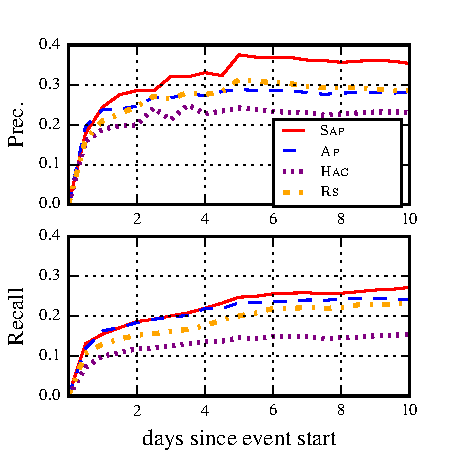
\includegraphics[scale=1.0]{feature_based_salience_models/figures/rouge-timev2.pdf}
   % %LaTeX with PSTricks extensions
%%Creator: inkscape 0.48.4
%%Please note this file requires PSTricks extensions
\psset{xunit=.5pt,yunit=.5pt,runit=.5pt}
\begin{pspicture}(272.8374939,270)
{
\newrgbcolor{curcolor}{1 1 1}
\pscustom[linestyle=none,fillstyle=solid,fillcolor=curcolor]
{
\newpath
\moveto(0.17431625,0)
\lineto(273.0093125,0)
\lineto(273.0093125,269.98125)
\lineto(0.17431625,269.98125)
\lineto(0.17431625,0)
\closepath
}
}
{
\newrgbcolor{curcolor}{1 1 1}
\pscustom[linestyle=none,fillstyle=solid,fillcolor=curcolor]
{
\newpath
\moveto(41.099625,147.255)
\lineto(245.725875,147.255)
\lineto(245.725875,242.9825)
\lineto(41.099625,242.9825)
\lineto(41.099625,147.255)
\closepath
}
}
{
\newrgbcolor{curcolor}{1 0 0}
\pscustom[linewidth=1.2499975,linecolor=curcolor]
{
\newpath
\moveto(41.099625,147.255)
\lineto(51.331,189.96625)
\lineto(61.5625,205.7475)
\lineto(71.7935,213.18125)
\lineto(82.024875,215.61)
\lineto(92.256375,215.465)
\lineto(102.48775,224.05125)
\lineto(112.71875,223.88125)
\lineto(122.94975,226.4225)
\lineto(133.18125,224.615)
\lineto(143.4125,237.1075)
\lineto(153.64375,235.70875)
\lineto(163.875,235.33375)
\lineto(174.1075,235.5275)
\lineto(184.33875,233.94875)
\lineto(194.57,233.6425)
\lineto(204.80125,232.56625)
\lineto(215.03125,233.30125)
\lineto(225.26375,233.85)
\lineto(235.49375,233.2875)
\lineto(245.725,231.94875)
}
}
{
\newrgbcolor{curcolor}{0 0 1}
\pscustom[linewidth=1.2499975,linecolor=curcolor,linestyle=dashed,dash=59.9998 59.9998]
{
\newpath
\moveto(41.099625,147.255)
\lineto(51.331,194.35125)
\lineto(61.5625,204.1)
\lineto(71.7935,204.53125)
\lineto(82.024875,206.305)
\lineto(92.256375,211.61375)
\lineto(102.48775,211.1375)
\lineto(112.71875,214.0875)
\lineto(122.94975,212.435)
\lineto(133.18125,215.13)
\lineto(143.4125,216.29875)
\lineto(153.64375,215.71)
\lineto(163.875,215.96625)
\lineto(174.1075,215.46875)
\lineto(184.33875,214.50375)
\lineto(194.57,213.40375)
\lineto(204.80125,214.08375)
\lineto(215.03125,214.5675)
\lineto(225.26375,214.6)
\lineto(235.49375,214.2125)
\lineto(245.725,214.27875)
}
}
{
\newrgbcolor{curcolor}{0.50196081 0 0.50196081}
\pscustom[linewidth=2.5,linecolor=curcolor,linestyle=dashed,dash=9.99998 30]
{
\newpath
\moveto(41.099625,147.255)
\lineto(51.331,185.32625)
\lineto(61.5625,192.445)
\lineto(71.7935,194.42375)
\lineto(82.024875,195.0475)
\lineto(92.256375,205.08)
\lineto(102.48775,198.10125)
\lineto(112.71875,207.02375)
\lineto(122.94975,201.695)
\lineto(133.18125,203.38125)
\lineto(143.4125,205.19625)
\lineto(153.64375,204.37125)
\lineto(163.875,202.99)
\lineto(174.1075,202.6875)
\lineto(184.33875,202.43375)
\lineto(194.57,200.83125)
\lineto(204.80125,201.6525)
\lineto(215.03125,202.2625)
\lineto(225.26375,202.82125)
\lineto(235.49375,202.7725)
\lineto(245.725,202.715)
}
}
{
\newrgbcolor{curcolor}{1 0.64705884 0}
\pscustom[linewidth=2.5,linecolor=curcolor,linestyle=dashed,dash=30 50 9.99998 50]
{
\newpath
\moveto(41.099625,147.255)
\lineto(51.331,186.37125)
\lineto(61.5625,197.48125)
\lineto(71.7935,201.68125)
\lineto(82.024875,206.16375)
\lineto(92.256375,212.23375)
\lineto(102.48775,210.5075)
\lineto(112.71875,214.53875)
\lineto(122.94975,213.30875)
\lineto(133.18125,215.02875)
\lineto(143.4125,222.195)
\lineto(153.64375,221.3)
\lineto(163.875,220.425)
\lineto(174.1075,219.85)
\lineto(184.33875,218.08)
\lineto(194.57,217.54)
\lineto(204.80125,217.29875)
\lineto(215.03125,217.2525)
\lineto(225.26375,216.625)
\lineto(235.49375,215.685)
\lineto(245.725,215.43625)
}
}
{
\newrgbcolor{curcolor}{0 0 0}
\pscustom[linewidth=1.2499975,linecolor=curcolor]
{
\newpath
\moveto(41.099625,242.9825)
\lineto(245.725,242.9825)
}
}
{
\newrgbcolor{curcolor}{0 0 0}
\pscustom[linewidth=1.2499975,linecolor=curcolor]
{
\newpath
\moveto(245.725,147.255)
\lineto(245.725,242.9825)
}
}
{
\newrgbcolor{curcolor}{0 0 0}
\pscustom[linewidth=1.2499975,linecolor=curcolor]
{
\newpath
\moveto(41.099625,147.255)
\lineto(245.725,147.255)
}
}
{
\newrgbcolor{curcolor}{0 0 0}
\pscustom[linewidth=1.2499975,linecolor=curcolor]
{
\newpath
\moveto(41.099625,147.255)
\lineto(41.099625,242.9825)
}
}
{
\newrgbcolor{curcolor}{0 0 0}
\pscustom[linewidth=0.625,linecolor=curcolor,linestyle=dashed,dash=9.99998 30]
{
\newpath
\moveto(82.024875,147.255)
\lineto(82.024875,242.9825)
}
}
{
\newrgbcolor{curcolor}{0 0 0}
\pscustom[linestyle=none,fillstyle=solid,fillcolor=curcolor]
{
\newpath
\moveto(82.024875,147.255)
\lineto(82.024875,152.25375)
}
}
{
\newrgbcolor{curcolor}{0 0 0}
\pscustom[linewidth=0.625,linecolor=curcolor]
{
\newpath
\moveto(82.024875,147.255)
\lineto(82.024875,152.25375)
}
}
{
\newrgbcolor{curcolor}{0 0 0}
\pscustom[linestyle=none,fillstyle=solid,fillcolor=curcolor]
{
\newpath
\moveto(82.024875,242.9825)
\lineto(82.024875,237.98125)
}
}
{
\newrgbcolor{curcolor}{0 0 0}
\pscustom[linewidth=0.625,linecolor=curcolor]
{
\newpath
\moveto(82.024875,242.9825)
\lineto(82.024875,237.98125)
}
}
{
\newrgbcolor{curcolor}{0 0 0}
\pscustom[linewidth=0.625,linecolor=curcolor,linestyle=dashed,dash=9.99998 30]
{
\newpath
\moveto(122.94975,147.255)
\lineto(122.94975,242.9825)
}
}
{
\newrgbcolor{curcolor}{0 0 0}
\pscustom[linestyle=none,fillstyle=solid,fillcolor=curcolor]
{
\newpath
\moveto(122.94975,147.255)
\lineto(122.94975,152.25375)
}
}
{
\newrgbcolor{curcolor}{0 0 0}
\pscustom[linewidth=0.625,linecolor=curcolor]
{
\newpath
\moveto(122.94975,147.255)
\lineto(122.94975,152.25375)
}
}
{
\newrgbcolor{curcolor}{0 0 0}
\pscustom[linestyle=none,fillstyle=solid,fillcolor=curcolor]
{
\newpath
\moveto(122.94975,242.9825)
\lineto(122.94975,237.98125)
}
}
{
\newrgbcolor{curcolor}{0 0 0}
\pscustom[linewidth=0.625,linecolor=curcolor]
{
\newpath
\moveto(122.94975,242.9825)
\lineto(122.94975,237.98125)
}
}
{
\newrgbcolor{curcolor}{0 0 0}
\pscustom[linewidth=0.625,linecolor=curcolor,linestyle=dashed,dash=9.99998 30]
{
\newpath
\moveto(163.875,147.255)
\lineto(163.875,242.9825)
}
}
{
\newrgbcolor{curcolor}{0 0 0}
\pscustom[linestyle=none,fillstyle=solid,fillcolor=curcolor]
{
\newpath
\moveto(163.875,147.255)
\lineto(163.875,152.25375)
}
}
{
\newrgbcolor{curcolor}{0 0 0}
\pscustom[linewidth=0.625,linecolor=curcolor]
{
\newpath
\moveto(163.875,147.255)
\lineto(163.875,152.25375)
}
}
{
\newrgbcolor{curcolor}{0 0 0}
\pscustom[linestyle=none,fillstyle=solid,fillcolor=curcolor]
{
\newpath
\moveto(163.875,242.9825)
\lineto(163.875,237.98125)
}
}
{
\newrgbcolor{curcolor}{0 0 0}
\pscustom[linewidth=0.625,linecolor=curcolor]
{
\newpath
\moveto(163.875,242.9825)
\lineto(163.875,237.98125)
}
}
{
\newrgbcolor{curcolor}{0 0 0}
\pscustom[linewidth=0.625,linecolor=curcolor,linestyle=dashed,dash=9.99998 30]
{
\newpath
\moveto(204.80125,147.255)
\lineto(204.80125,242.9825)
}
}
{
\newrgbcolor{curcolor}{0 0 0}
\pscustom[linestyle=none,fillstyle=solid,fillcolor=curcolor]
{
\newpath
\moveto(204.80125,147.255)
\lineto(204.80125,152.25375)
}
}
{
\newrgbcolor{curcolor}{0 0 0}
\pscustom[linewidth=0.625,linecolor=curcolor]
{
\newpath
\moveto(204.80125,147.255)
\lineto(204.80125,152.25375)
}
}
{
\newrgbcolor{curcolor}{0 0 0}
\pscustom[linestyle=none,fillstyle=solid,fillcolor=curcolor]
{
\newpath
\moveto(204.80125,242.9825)
\lineto(204.80125,237.98125)
}
}
{
\newrgbcolor{curcolor}{0 0 0}
\pscustom[linewidth=0.625,linecolor=curcolor]
{
\newpath
\moveto(204.80125,242.9825)
\lineto(204.80125,237.98125)
}
}
{
\newrgbcolor{curcolor}{0 0 0}
\pscustom[linewidth=0.625,linecolor=curcolor,linestyle=dashed,dash=9.99998 30]
{
\newpath
\moveto(245.725,147.255)
\lineto(245.725,242.9825)
}
}
{
\newrgbcolor{curcolor}{0 0 0}
\pscustom[linestyle=none,fillstyle=solid,fillcolor=curcolor]
{
\newpath
\moveto(245.725,147.255)
\lineto(245.725,152.25375)
}
}
{
\newrgbcolor{curcolor}{0 0 0}
\pscustom[linewidth=0.625,linecolor=curcolor]
{
\newpath
\moveto(245.725,147.255)
\lineto(245.725,152.25375)
}
}
{
\newrgbcolor{curcolor}{0 0 0}
\pscustom[linestyle=none,fillstyle=solid,fillcolor=curcolor]
{
\newpath
\moveto(245.725,242.9825)
\lineto(245.725,237.98125)
}
}
{
\newrgbcolor{curcolor}{0 0 0}
\pscustom[linewidth=0.625,linecolor=curcolor]
{
\newpath
\moveto(245.725,242.9825)
\lineto(245.725,237.98125)
}
}
{
\newrgbcolor{curcolor}{0 0 0}
\pscustom[linewidth=0.625,linecolor=curcolor,linestyle=dashed,dash=9.99998 30]
{
\newpath
\moveto(41.099625,147.255)
\lineto(245.725,147.255)
}
}
{
\newrgbcolor{curcolor}{0 0 0}
\pscustom[linestyle=none,fillstyle=solid,fillcolor=curcolor]
{
\newpath
\moveto(41.099625,147.255)
\lineto(46.099625,147.255)
}
}
{
\newrgbcolor{curcolor}{0 0 0}
\pscustom[linewidth=0.625,linecolor=curcolor]
{
\newpath
\moveto(41.099625,147.255)
\lineto(46.099625,147.255)
}
}
{
\newrgbcolor{curcolor}{0 0 0}
\pscustom[linestyle=none,fillstyle=solid,fillcolor=curcolor]
{
\newpath
\moveto(245.725,147.255)
\lineto(240.725,147.255)
}
}
{
\newrgbcolor{curcolor}{0 0 0}
\pscustom[linewidth=0.625,linecolor=curcolor]
{
\newpath
\moveto(245.725,147.255)
\lineto(240.725,147.255)
}
}
{
\newrgbcolor{curcolor}{0 0 0}
\pscustom[linewidth=0.625,linecolor=curcolor,linestyle=dashed,dash=9.99998 30]
{
\newpath
\moveto(41.099625,171.1875)
\lineto(245.725,171.1875)
}
}
{
\newrgbcolor{curcolor}{0 0 0}
\pscustom[linestyle=none,fillstyle=solid,fillcolor=curcolor]
{
\newpath
\moveto(41.099625,171.1875)
\lineto(46.099625,171.1875)
}
}
{
\newrgbcolor{curcolor}{0 0 0}
\pscustom[linewidth=0.625,linecolor=curcolor]
{
\newpath
\moveto(41.099625,171.1875)
\lineto(46.099625,171.1875)
}
}
{
\newrgbcolor{curcolor}{0 0 0}
\pscustom[linestyle=none,fillstyle=solid,fillcolor=curcolor]
{
\newpath
\moveto(245.725,171.1875)
\lineto(240.725,171.1875)
}
}
{
\newrgbcolor{curcolor}{0 0 0}
\pscustom[linewidth=0.625,linecolor=curcolor]
{
\newpath
\moveto(245.725,171.1875)
\lineto(240.725,171.1875)
}
}
{
\newrgbcolor{curcolor}{0 0 0}
\pscustom[linewidth=0.625,linecolor=curcolor,linestyle=dashed,dash=9.99998 30]
{
\newpath
\moveto(41.099625,195.1175)
\lineto(245.725,195.1175)
}
}
{
\newrgbcolor{curcolor}{0 0 0}
\pscustom[linestyle=none,fillstyle=solid,fillcolor=curcolor]
{
\newpath
\moveto(41.099625,195.1175)
\lineto(46.099625,195.1175)
}
}
{
\newrgbcolor{curcolor}{0 0 0}
\pscustom[linewidth=0.625,linecolor=curcolor]
{
\newpath
\moveto(41.099625,195.1175)
\lineto(46.099625,195.1175)
}
}
{
\newrgbcolor{curcolor}{0 0 0}
\pscustom[linestyle=none,fillstyle=solid,fillcolor=curcolor]
{
\newpath
\moveto(245.725,195.1175)
\lineto(240.725,195.1175)
}
}
{
\newrgbcolor{curcolor}{0 0 0}
\pscustom[linewidth=0.625,linecolor=curcolor]
{
\newpath
\moveto(245.725,195.1175)
\lineto(240.725,195.1175)
}
}
{
\newrgbcolor{curcolor}{0 0 0}
\pscustom[linewidth=0.625,linecolor=curcolor,linestyle=dashed,dash=9.99998 30]
{
\newpath
\moveto(41.099625,219.05)
\lineto(245.725,219.05)
}
}
{
\newrgbcolor{curcolor}{0 0 0}
\pscustom[linestyle=none,fillstyle=solid,fillcolor=curcolor]
{
\newpath
\moveto(41.099625,219.05)
\lineto(46.099625,219.05)
}
}
{
\newrgbcolor{curcolor}{0 0 0}
\pscustom[linewidth=0.625,linecolor=curcolor]
{
\newpath
\moveto(41.099625,219.05)
\lineto(46.099625,219.05)
}
}
{
\newrgbcolor{curcolor}{0 0 0}
\pscustom[linestyle=none,fillstyle=solid,fillcolor=curcolor]
{
\newpath
\moveto(245.725,219.05)
\lineto(240.725,219.05)
}
}
{
\newrgbcolor{curcolor}{0 0 0}
\pscustom[linewidth=0.625,linecolor=curcolor]
{
\newpath
\moveto(245.725,219.05)
\lineto(240.725,219.05)
}
}
{
\newrgbcolor{curcolor}{0 0 0}
\pscustom[linewidth=0.625,linecolor=curcolor,linestyle=dashed,dash=9.99998 30]
{
\newpath
\moveto(41.099625,242.9825)
\lineto(245.725,242.9825)
}
}
{
\newrgbcolor{curcolor}{0 0 0}
\pscustom[linestyle=none,fillstyle=solid,fillcolor=curcolor]
{
\newpath
\moveto(41.099625,242.9825)
\lineto(46.099625,242.9825)
}
}
{
\newrgbcolor{curcolor}{0 0 0}
\pscustom[linewidth=0.625,linecolor=curcolor]
{
\newpath
\moveto(41.099625,242.9825)
\lineto(46.099625,242.9825)
}
}
{
\newrgbcolor{curcolor}{0 0 0}
\pscustom[linestyle=none,fillstyle=solid,fillcolor=curcolor]
{
\newpath
\moveto(245.725,242.9825)
\lineto(240.725,242.9825)
}
}
{
\newrgbcolor{curcolor}{0 0 0}
\pscustom[linewidth=0.625,linecolor=curcolor]
{
\newpath
\moveto(245.725,242.9825)
\lineto(240.725,242.9825)
}
}
{
\newrgbcolor{curcolor}{1 1 1}
\pscustom[linestyle=none,fillstyle=solid,fillcolor=curcolor]
{
\newpath
\moveto(163.875,146.29625)
\lineto(240.965375,146.29625)
\lineto(240.965375,198.470125)
\lineto(163.875,198.470125)
\lineto(163.875,146.29625)
\closepath
}
}
{
\newrgbcolor{curcolor}{0 0 0}
\pscustom[linewidth=1.2499975,linecolor=curcolor]
{
\newpath
\moveto(163.875,146.29625)
\lineto(240.965375,146.29625)
\lineto(240.965375,198.470125)
\lineto(163.875,198.470125)
\lineto(163.875,146.29625)
\closepath
}
}
{
\newrgbcolor{curcolor}{1 0 0}
\pscustom[linewidth=1.2499975,linecolor=curcolor]
{
\newpath
\moveto(170,191.90875)
\lineto(182.25125,191.90875)
}
}
{
\newrgbcolor{curcolor}{0 0 1}
\pscustom[linewidth=1.2499975,linecolor=curcolor,linestyle=dashed,dash=59.9998 59.9998]
{
\newpath
\moveto(170,179.52125)
\lineto(182.25125,179.52125)
}
}
{
\newrgbcolor{curcolor}{0.50196081 0 0.50196081}
\pscustom[linewidth=2.5,linecolor=curcolor,linestyle=dashed,dash=9.99998 30]
{
\newpath
\moveto(170,167.13375)
\lineto(182.25125,167.13375)
}
}
{
\newrgbcolor{curcolor}{1 0.64705884 0}
\pscustom[linewidth=2.5,linecolor=curcolor,linestyle=dashed,dash=30 50 9.99998 50]
{
\newpath
\moveto(170,154.74625)
\lineto(182.25125,154.74625)
}
}
{
\newrgbcolor{curcolor}{1 1 1}
\pscustom[linestyle=none,fillstyle=solid,fillcolor=curcolor]
{
\newpath
\moveto(41.099625,32.381375)
\lineto(245.725875,32.381375)
\lineto(245.725875,128.109375)
\lineto(41.099625,128.109375)
\lineto(41.099625,32.381375)
\closepath
}
}
{
\newrgbcolor{curcolor}{1 0 0}
\pscustom[linewidth=1.2499975,linecolor=curcolor]
{
\newpath
\moveto(41.099625,32.381375)
\lineto(51.331,63.75925)
\lineto(61.5625,69.5825)
\lineto(71.7935,73.40625)
\lineto(82.024875,77.004875)
\lineto(92.256375,78.454125)
\lineto(102.48775,80.4385)
\lineto(112.71875,82.2495)
\lineto(122.94975,85.096625)
\lineto(133.18125,88.106)
\lineto(143.4125,91.709)
\lineto(153.64375,92.204125)
\lineto(163.875,93.765125)
\lineto(174.1075,94.13625)
\lineto(184.33875,94.338875)
\lineto(194.57,93.653375)
\lineto(204.80125,94.041)
\lineto(215.03125,95.014125)
\lineto(225.26375,95.994625)
\lineto(235.49375,96.437)
\lineto(245.725,97.587375)
}
}
{
\newrgbcolor{curcolor}{0 0 1}
\pscustom[linewidth=1.2499975,linecolor=curcolor,linestyle=dashed,dash=59.9998 59.9998]
{
\newpath
\moveto(41.099625,32.381375)
\lineto(51.331,60.8775)
\lineto(61.5625,71.483875)
\lineto(71.7935,73.48925)
\lineto(82.024875,76.46725)
\lineto(92.256375,78.42675)
\lineto(102.48775,79.755375)
\lineto(112.71875,80.754875)
\lineto(122.94975,84.814)
\lineto(133.18125,84.84175)
\lineto(143.4125,88.27925)
\lineto(153.64375,88.40825)
\lineto(163.875,89.34225)
\lineto(174.1075,89.2935)
\lineto(184.33875,90.023)
\lineto(194.57,89.84375)
\lineto(204.80125,90.451125)
\lineto(215.03125,90.921375)
\lineto(225.26375,90.911125)
\lineto(235.49375,90.497125)
\lineto(245.725,90.536125)
}
}
{
\newrgbcolor{curcolor}{0.50196081 0 0.50196081}
\pscustom[linewidth=2.5,linecolor=curcolor,linestyle=dashed,dash=9.99998 30]
{
\newpath
\moveto(41.099625,32.381375)
\lineto(51.331,49.727)
\lineto(61.5625,56.4385)
\lineto(71.7935,58.316375)
\lineto(82.024875,60.792)
\lineto(92.256375,61.2515)
\lineto(102.48775,62.370125)
\lineto(112.71875,63.806625)
\lineto(122.94975,64.995625)
\lineto(133.18125,65.338875)
\lineto(143.4125,67.34425)
\lineto(153.64375,66.870125)
\lineto(163.875,67.945375)
\lineto(174.1075,67.8955)
\lineto(184.33875,67.995625)
\lineto(194.57,66.8325)
\lineto(204.80125,67.40675)
\lineto(215.03125,67.71875)
\lineto(225.26375,68.557625)
\lineto(235.49375,68.90775)
\lineto(245.725,69.161625)
}
}
{
\newrgbcolor{curcolor}{1 0.64705884 0}
\pscustom[linewidth=2.5,linecolor=curcolor,linestyle=dashed,dash=30 50 9.99998 50]
{
\newpath
\moveto(41.099625,32.381375)
\lineto(51.331,57.860375)
\lineto(61.5625,63.611375)
\lineto(71.7935,66.570375)
\lineto(82.024875,68.849625)
\lineto(92.256375,69.753375)
\lineto(102.48775,71.26175)
\lineto(112.71875,72.3315)
\lineto(122.94975,74.507875)
\lineto(133.18125,78.09275)
\lineto(143.4125,80.444875)
\lineto(153.64375,82.15775)
\lineto(163.875,85.014625)
\lineto(174.1075,84.90875)
\lineto(184.33875,85.557625)
\lineto(194.57,84.9815)
\lineto(204.80125,85.49025)
\lineto(215.03125,87.107875)
\lineto(225.26375,87.3985)
\lineto(235.49375,87.50925)
\lineto(245.725,88.1435)
}
}
{
\newrgbcolor{curcolor}{0 0 0}
\pscustom[linewidth=1.2499975,linecolor=curcolor]
{
\newpath
\moveto(41.099625,128.10875)
\lineto(245.725,128.10875)
}
}
{
\newrgbcolor{curcolor}{0 0 0}
\pscustom[linewidth=1.2499975,linecolor=curcolor]
{
\newpath
\moveto(245.725,32.381375)
\lineto(245.725,128.10875)
}
}
{
\newrgbcolor{curcolor}{0 0 0}
\pscustom[linewidth=1.2499975,linecolor=curcolor]
{
\newpath
\moveto(41.099625,32.381375)
\lineto(245.725,32.381375)
}
}
{
\newrgbcolor{curcolor}{0 0 0}
\pscustom[linewidth=1.2499975,linecolor=curcolor]
{
\newpath
\moveto(41.099625,32.381375)
\lineto(41.099625,128.10875)
}
}
{
\newrgbcolor{curcolor}{0 0 0}
\pscustom[linewidth=0.625,linecolor=curcolor,linestyle=dashed,dash=9.99998 30]
{
\newpath
\moveto(82.024875,32.381375)
\lineto(82.024875,128.10875)
}
}
{
\newrgbcolor{curcolor}{0 0 0}
\pscustom[linestyle=none,fillstyle=solid,fillcolor=curcolor]
{
\newpath
\moveto(82.024875,32.381375)
\lineto(82.024875,37.381375)
}
}
{
\newrgbcolor{curcolor}{0 0 0}
\pscustom[linewidth=0.625,linecolor=curcolor]
{
\newpath
\moveto(82.024875,32.381375)
\lineto(82.024875,37.381375)
}
}
{
\newrgbcolor{curcolor}{0 0 0}
\pscustom[linestyle=none,fillstyle=solid,fillcolor=curcolor]
{
\newpath
\moveto(82.024875,128.10875)
\lineto(82.024875,123.108875)
}
}
{
\newrgbcolor{curcolor}{0 0 0}
\pscustom[linewidth=0.625,linecolor=curcolor]
{
\newpath
\moveto(82.024875,128.10875)
\lineto(82.024875,123.108875)
}
}
{
\newrgbcolor{curcolor}{0 0 0}
\pscustom[linewidth=0.625,linecolor=curcolor,linestyle=dashed,dash=9.99998 30]
{
\newpath
\moveto(122.94975,32.381375)
\lineto(122.94975,128.10875)
}
}
{
\newrgbcolor{curcolor}{0 0 0}
\pscustom[linestyle=none,fillstyle=solid,fillcolor=curcolor]
{
\newpath
\moveto(122.94975,32.381375)
\lineto(122.94975,37.381375)
}
}
{
\newrgbcolor{curcolor}{0 0 0}
\pscustom[linewidth=0.625,linecolor=curcolor]
{
\newpath
\moveto(122.94975,32.381375)
\lineto(122.94975,37.381375)
}
}
{
\newrgbcolor{curcolor}{0 0 0}
\pscustom[linestyle=none,fillstyle=solid,fillcolor=curcolor]
{
\newpath
\moveto(122.94975,128.10875)
\lineto(122.94975,123.108875)
}
}
{
\newrgbcolor{curcolor}{0 0 0}
\pscustom[linewidth=0.625,linecolor=curcolor]
{
\newpath
\moveto(122.94975,128.10875)
\lineto(122.94975,123.108875)
}
}
{
\newrgbcolor{curcolor}{0 0 0}
\pscustom[linewidth=0.625,linecolor=curcolor,linestyle=dashed,dash=9.99998 30]
{
\newpath
\moveto(163.875,32.381375)
\lineto(163.875,128.10875)
}
}
{
\newrgbcolor{curcolor}{0 0 0}
\pscustom[linestyle=none,fillstyle=solid,fillcolor=curcolor]
{
\newpath
\moveto(163.875,32.381375)
\lineto(163.875,37.381375)
}
}
{
\newrgbcolor{curcolor}{0 0 0}
\pscustom[linewidth=0.625,linecolor=curcolor]
{
\newpath
\moveto(163.875,32.381375)
\lineto(163.875,37.381375)
}
}
{
\newrgbcolor{curcolor}{0 0 0}
\pscustom[linestyle=none,fillstyle=solid,fillcolor=curcolor]
{
\newpath
\moveto(163.875,128.10875)
\lineto(163.875,123.108875)
}
}
{
\newrgbcolor{curcolor}{0 0 0}
\pscustom[linewidth=0.625,linecolor=curcolor]
{
\newpath
\moveto(163.875,128.10875)
\lineto(163.875,123.108875)
}
}
{
\newrgbcolor{curcolor}{0 0 0}
\pscustom[linewidth=0.625,linecolor=curcolor,linestyle=dashed,dash=9.99998 30]
{
\newpath
\moveto(204.80125,32.381375)
\lineto(204.80125,128.10875)
}
}
{
\newrgbcolor{curcolor}{0 0 0}
\pscustom[linestyle=none,fillstyle=solid,fillcolor=curcolor]
{
\newpath
\moveto(204.80125,32.381375)
\lineto(204.80125,37.381375)
}
}
{
\newrgbcolor{curcolor}{0 0 0}
\pscustom[linewidth=0.625,linecolor=curcolor]
{
\newpath
\moveto(204.80125,32.381375)
\lineto(204.80125,37.381375)
}
}
{
\newrgbcolor{curcolor}{0 0 0}
\pscustom[linestyle=none,fillstyle=solid,fillcolor=curcolor]
{
\newpath
\moveto(204.80125,128.10875)
\lineto(204.80125,123.108875)
}
}
{
\newrgbcolor{curcolor}{0 0 0}
\pscustom[linewidth=0.625,linecolor=curcolor]
{
\newpath
\moveto(204.80125,128.10875)
\lineto(204.80125,123.108875)
}
}
{
\newrgbcolor{curcolor}{0 0 0}
\pscustom[linewidth=0.625,linecolor=curcolor,linestyle=dashed,dash=9.99998 30]
{
\newpath
\moveto(245.725,32.381375)
\lineto(245.725,128.10875)
}
}
{
\newrgbcolor{curcolor}{0 0 0}
\pscustom[linestyle=none,fillstyle=solid,fillcolor=curcolor]
{
\newpath
\moveto(245.725,32.381375)
\lineto(245.725,37.381375)
}
}
{
\newrgbcolor{curcolor}{0 0 0}
\pscustom[linewidth=0.625,linecolor=curcolor]
{
\newpath
\moveto(245.725,32.381375)
\lineto(245.725,37.381375)
}
}
{
\newrgbcolor{curcolor}{0 0 0}
\pscustom[linestyle=none,fillstyle=solid,fillcolor=curcolor]
{
\newpath
\moveto(245.725,128.10875)
\lineto(245.725,123.108875)
}
}
{
\newrgbcolor{curcolor}{0 0 0}
\pscustom[linewidth=0.625,linecolor=curcolor]
{
\newpath
\moveto(245.725,128.10875)
\lineto(245.725,123.108875)
}
}
{
\newrgbcolor{curcolor}{0 0 0}
\pscustom[linewidth=0.625,linecolor=curcolor,linestyle=dashed,dash=9.99998 30]
{
\newpath
\moveto(41.099625,32.381375)
\lineto(245.725,32.381375)
}
}
{
\newrgbcolor{curcolor}{0 0 0}
\pscustom[linestyle=none,fillstyle=solid,fillcolor=curcolor]
{
\newpath
\moveto(41.099625,32.381375)
\lineto(46.099625,32.381375)
}
}
{
\newrgbcolor{curcolor}{0 0 0}
\pscustom[linewidth=0.625,linecolor=curcolor]
{
\newpath
\moveto(41.099625,32.381375)
\lineto(46.099625,32.381375)
}
}
{
\newrgbcolor{curcolor}{0 0 0}
\pscustom[linestyle=none,fillstyle=solid,fillcolor=curcolor]
{
\newpath
\moveto(245.725,32.381375)
\lineto(240.725,32.381375)
}
}
{
\newrgbcolor{curcolor}{0 0 0}
\pscustom[linewidth=0.625,linecolor=curcolor]
{
\newpath
\moveto(245.725,32.381375)
\lineto(240.725,32.381375)
}
}
{
\newrgbcolor{curcolor}{0 0 0}
\pscustom[linewidth=0.625,linecolor=curcolor,linestyle=dashed,dash=9.99998 30]
{
\newpath
\moveto(41.099625,56.3135)
\lineto(245.725,56.3135)
}
}
{
\newrgbcolor{curcolor}{0 0 0}
\pscustom[linestyle=none,fillstyle=solid,fillcolor=curcolor]
{
\newpath
\moveto(41.099625,56.3135)
\lineto(46.099625,56.3135)
}
}
{
\newrgbcolor{curcolor}{0 0 0}
\pscustom[linewidth=0.625,linecolor=curcolor]
{
\newpath
\moveto(41.099625,56.3135)
\lineto(46.099625,56.3135)
}
}
{
\newrgbcolor{curcolor}{0 0 0}
\pscustom[linestyle=none,fillstyle=solid,fillcolor=curcolor]
{
\newpath
\moveto(245.725,56.3135)
\lineto(240.725,56.3135)
}
}
{
\newrgbcolor{curcolor}{0 0 0}
\pscustom[linewidth=0.625,linecolor=curcolor]
{
\newpath
\moveto(245.725,56.3135)
\lineto(240.725,56.3135)
}
}
{
\newrgbcolor{curcolor}{0 0 0}
\pscustom[linewidth=0.625,linecolor=curcolor,linestyle=dashed,dash=9.99998 30]
{
\newpath
\moveto(41.099625,80.245125)
\lineto(245.725,80.245125)
}
}
{
\newrgbcolor{curcolor}{0 0 0}
\pscustom[linestyle=none,fillstyle=solid,fillcolor=curcolor]
{
\newpath
\moveto(41.099625,80.245125)
\lineto(46.099625,80.245125)
}
}
{
\newrgbcolor{curcolor}{0 0 0}
\pscustom[linewidth=0.625,linecolor=curcolor]
{
\newpath
\moveto(41.099625,80.245125)
\lineto(46.099625,80.245125)
}
}
{
\newrgbcolor{curcolor}{0 0 0}
\pscustom[linestyle=none,fillstyle=solid,fillcolor=curcolor]
{
\newpath
\moveto(245.725,80.245125)
\lineto(240.725,80.245125)
}
}
{
\newrgbcolor{curcolor}{0 0 0}
\pscustom[linewidth=0.625,linecolor=curcolor]
{
\newpath
\moveto(245.725,80.245125)
\lineto(240.725,80.245125)
}
}
{
\newrgbcolor{curcolor}{0 0 0}
\pscustom[linewidth=0.625,linecolor=curcolor,linestyle=dashed,dash=9.99998 30]
{
\newpath
\moveto(41.099625,104.17675)
\lineto(245.725,104.17675)
}
}
{
\newrgbcolor{curcolor}{0 0 0}
\pscustom[linestyle=none,fillstyle=solid,fillcolor=curcolor]
{
\newpath
\moveto(41.099625,104.17675)
\lineto(46.099625,104.17675)
}
}
{
\newrgbcolor{curcolor}{0 0 0}
\pscustom[linewidth=0.625,linecolor=curcolor]
{
\newpath
\moveto(41.099625,104.17675)
\lineto(46.099625,104.17675)
}
}
{
\newrgbcolor{curcolor}{0 0 0}
\pscustom[linestyle=none,fillstyle=solid,fillcolor=curcolor]
{
\newpath
\moveto(245.725,104.17675)
\lineto(240.725,104.17675)
}
}
{
\newrgbcolor{curcolor}{0 0 0}
\pscustom[linewidth=0.625,linecolor=curcolor]
{
\newpath
\moveto(245.725,104.17675)
\lineto(240.725,104.17675)
}
}
{
\newrgbcolor{curcolor}{0 0 0}
\pscustom[linewidth=0.625,linecolor=curcolor,linestyle=dashed,dash=9.99998 30]
{
\newpath
\moveto(41.099625,128.10875)
\lineto(245.725,128.10875)
}
}
{
\newrgbcolor{curcolor}{0 0 0}
\pscustom[linestyle=none,fillstyle=solid,fillcolor=curcolor]
{
\newpath
\moveto(41.099625,128.10875)
\lineto(46.099625,128.10875)
}
}
{
\newrgbcolor{curcolor}{0 0 0}
\pscustom[linewidth=0.625,linecolor=curcolor]
{
\newpath
\moveto(41.099625,128.10875)
\lineto(46.099625,128.10875)
}
}
{
\newrgbcolor{curcolor}{0 0 0}
\pscustom[linestyle=none,fillstyle=solid,fillcolor=curcolor]
{
\newpath
\moveto(245.725,128.10875)
\lineto(240.725,128.10875)
}
}
{
\newrgbcolor{curcolor}{0 0 0}
\pscustom[linewidth=0.625,linecolor=curcolor]
{
\newpath
\moveto(245.725,128.10875)
\lineto(240.725,128.10875)
}
}
{
\newrgbcolor{curcolor}{0.13725491 0.12156863 0.1254902}
\pscustom[linestyle=none,fillstyle=solid,fillcolor=curcolor]
{
\newpath
\moveto(-102.590125,403.91625)
\lineto(0.159875,403.91625)
\lineto(0.159875,404.51625)
\lineto(-102.590125,404.51625)
\closepath
}
}
{
\newrgbcolor{curcolor}{0 0 0}
\pscustom[linestyle=none,fillstyle=solid,fillcolor=curcolor]
{
\newpath
\moveto(84.26686296,136.86487786)
\lineto(84.13734901,136.91469093)
\curveto(83.76873273,136.3468226)(83.63921795,136.25715852)(83.19090085,136.25715852)
\lineto(80.80983655,136.25715852)
\lineto(82.48355539,138.01057826)
\curveto(83.37022698,138.93710027)(83.75876974,139.69426049)(83.75876974,140.47134346)
\curveto(83.75876974,141.46760368)(82.95179712,142.23472581)(81.9156865,142.23472581)
\curveto(81.36774338,142.23472581)(80.84968663,142.01554795)(80.48107035,141.61704386)
\curveto(80.16226708,141.27831539)(80.01282741,140.95951075)(79.84346317,140.252166)
\lineto(80.05267802,140.20235294)
\curveto(80.45118211,141.17868795)(80.80983724,141.49749252)(81.49725679,141.49749252)
\curveto(82.33411537,141.49749252)(82.9019851,140.92962279)(82.9019851,140.0927642)
\curveto(82.9019851,139.31568123)(82.4437041,138.38915664)(81.60684552,137.50248504)
\lineto(79.83350056,135.61955135)
\lineto(79.83350056,135.5)
\lineto(83.7189193,135.5)
\lineto(84.26686296,136.86487786)
}
}
{
\newrgbcolor{curcolor}{0 0 0}
\pscustom[linestyle=none,fillstyle=solid,fillcolor=curcolor]
{
\newpath
\moveto(125.16179507,137.80136341)
\lineto(124.14560863,137.80136341)
\lineto(124.14560863,142.23472581)
\lineto(123.7072537,142.23472581)
\lineto(120.57899348,137.80136341)
\lineto(120.57899348,137.16375623)
\lineto(123.3784875,137.16375623)
\lineto(123.3784875,135.5)
\lineto(124.14560863,135.5)
\lineto(124.14560863,137.16375623)
\lineto(125.16179507,137.16375623)
\lineto(125.16179507,137.80136341)
\moveto(123.36852489,137.80136341)
\lineto(120.97749797,137.80136341)
\lineto(123.36852489,141.21853938)
\lineto(123.36852489,137.80136341)
}
}
{
\newrgbcolor{curcolor}{0 0 0}
\pscustom[linestyle=none,fillstyle=solid,fillcolor=curcolor]
{
\newpath
\moveto(165.82757185,142.39499312)
\curveto(164.6918352,142.2953671)(164.11400183,142.10607686)(163.38673187,141.59798415)
\curveto(162.31077083,140.83086378)(161.72297564,139.69512389)(161.72297564,138.3601352)
\curveto(161.72297564,137.49338881)(161.9919666,136.61667757)(162.42035849,136.11854746)
\curveto(162.79893737,135.68019297)(163.33691943,135.44108984)(163.95460076,135.44108984)
\curveto(165.18996343,135.44108984)(166.04674931,136.38753937)(166.04674931,137.76237847)
\curveto(166.04674931,139.03759155)(165.31947748,139.84456441)(164.17377823,139.84456441)
\curveto(163.73542373,139.84456441)(163.52620781,139.77482574)(162.89856387,139.39624686)
\curveto(163.16755413,140.90059979)(164.28336853,141.97656367)(165.84749707,142.23559132)
\lineto(165.82757185,142.39499312)
\moveto(163.79519897,139.38628425)
\curveto(164.65198276,139.38628425)(165.15011422,138.66897493)(165.15011422,137.42364965)
\curveto(165.15011422,136.32776341)(164.76157165,135.72004298)(164.0641895,135.72004298)
\curveto(163.1874805,135.72004298)(162.64949857,136.65653006)(162.64949857,138.2007334)
\curveto(162.64949857,138.70882611)(162.72919967,138.98777991)(162.92845171,139.13721894)
\curveto(163.13766636,139.29662058)(163.44650789,139.38628425)(163.79519897,139.38628425)
}
}
{
\newrgbcolor{curcolor}{0 0 0}
\pscustom[linestyle=none,fillstyle=solid,fillcolor=curcolor]
{
\newpath
\moveto(205.1982243,139.27669551)
\curveto(206.18452191,139.80471343)(206.53321432,140.22314435)(206.53321432,140.9006013)
\curveto(206.53321432,141.71753468)(205.81590525,142.31529222)(204.81964503,142.31529222)
\curveto(203.7337214,142.31529222)(202.92674873,141.6477963)(202.92674873,140.7411995)
\curveto(202.92674873,140.09363036)(203.1160394,139.80471304)(204.16211263,138.88815364)
\curveto(203.0861516,138.07122026)(202.86697305,137.76237779)(202.86697305,137.08492084)
\curveto(202.86697305,136.11854843)(203.65402054,135.44108984)(204.77979459,135.44108984)
\curveto(205.97530685,135.44108984)(206.74242918,136.09862326)(206.74242918,137.12477129)
\curveto(206.74242918,137.89189166)(206.40369916,138.38006132)(205.1982243,139.27669551)
\moveto(205.01889728,138.25054646)
\curveto(205.74616724,137.73249115)(205.98527066,137.37383604)(205.98527066,136.81593031)
\curveto(205.98527066,136.16836117)(205.53695246,135.72004298)(204.88938332,135.72004298)
\curveto(204.13222555,135.72004298)(203.62413158,136.29787535)(203.62413158,137.16462174)
\curveto(203.62413158,137.80222828)(203.84330962,138.22065909)(204.42114055,138.6889014)
\lineto(205.01889728,138.25054646)
\moveto(204.90930854,139.45602253)
\curveto(204.02263695,140.03385346)(203.66398203,140.49213476)(203.66398203,141.05004048)
\curveto(203.66398203,141.6278714)(204.1123002,142.03633908)(204.73994414,142.03633908)
\curveto(205.41740109,142.03633908)(205.84579409,141.59798346)(205.84579409,140.91056391)
\curveto(205.84579409,140.34269558)(205.56684038,139.89437709)(204.99897205,139.51579821)
\curveto(204.94915904,139.4859104)(204.94915895,139.48591034)(204.90930854,139.45602253)
}
}
{
\newrgbcolor{curcolor}{0 0 0}
\pscustom[linestyle=none,fillstyle=solid,fillcolor=curcolor]
{
\newpath
\moveto(243.64275722,142.31529222)
\lineto(241.84948703,141.40869452)
\lineto(241.84948703,141.26921795)
\curveto(241.96903826,141.31903096)(242.07862715,141.35888147)(242.11847756,141.37880668)
\curveto(242.2978044,141.44854489)(242.46716909,141.48839541)(242.56679511,141.48839541)
\curveto(242.77600975,141.48839541)(242.86567347,141.33895591)(242.86567347,141.02015264)
\lineto(242.86567347,136.50708934)
\curveto(242.86567347,136.17832346)(242.78597242,135.94918297)(242.62657078,135.85951955)
\curveto(242.47713175,135.76985613)(242.33765461,135.73996819)(241.91922532,135.73000559)
\lineto(241.91922532,135.58056641)
\lineto(244.66890627,135.58056641)
\lineto(244.66890627,135.73000559)
\curveto(243.8818607,135.73996819)(243.72245812,135.8395948)(243.72245812,136.31779971)
\lineto(243.72245812,142.295367)
\lineto(243.64275722,142.31529222)
}
}
{
\newrgbcolor{curcolor}{0 0 0}
\pscustom[linestyle=none,fillstyle=solid,fillcolor=curcolor]
{
\newpath
\moveto(248.22432063,142.31529222)
\curveto(247.6763775,142.31529222)(247.25794688,142.14592747)(246.8893306,141.79723639)
\curveto(246.31149967,141.23933067)(245.93291983,140.09362855)(245.93291983,138.92800409)
\curveto(245.93291983,137.84208045)(246.2616865,136.67645319)(246.7299288,136.11854746)
\curveto(247.09854508,135.68019297)(247.60663925,135.44108984)(248.18447018,135.44108984)
\curveto(248.69256289,135.44108984)(249.12095608,135.61045459)(249.47960976,135.95914567)
\curveto(250.05744068,136.50708879)(250.43602052,137.66275355)(250.43602052,138.86822842)
\curveto(250.43602052,140.91056187)(249.52942151,142.31529222)(248.22432063,142.31529222)
\moveto(248.19443279,142.05626431)
\curveto(249.03129137,142.05626431)(249.47960976,140.93048705)(249.47960976,138.84830319)
\curveto(249.47960976,136.76611933)(249.04125396,135.70011775)(248.18447018,135.70011775)
\curveto(247.32768639,135.70011775)(246.8893306,136.76611932)(246.8893306,138.83834058)
\curveto(246.8893306,140.95041224)(247.337649,142.05626431)(248.19443279,142.05626431)
}
}
{
\newrgbcolor{curcolor}{0 0 0}
\pscustom[linestyle=none,fillstyle=solid,fillcolor=curcolor]
{
\newpath
\moveto(25.90725253,151.76988206)
\curveto(25.3593094,151.76988206)(24.94087878,151.60051731)(24.5722625,151.25182623)
\curveto(23.99443157,150.69392051)(23.61585173,149.54821839)(23.61585173,148.38259393)
\curveto(23.61585173,147.29667029)(23.9446184,146.13104303)(24.4128607,145.57313731)
\curveto(24.78147698,145.13478281)(25.28957115,144.89567968)(25.86740208,144.89567968)
\curveto(26.37549479,144.89567968)(26.80388798,145.06504444)(27.16254166,145.41373551)
\curveto(27.74037258,145.96167863)(28.11895242,147.1173434)(28.11895242,148.32281826)
\curveto(28.11895242,150.36515171)(27.21235341,151.76988206)(25.90725253,151.76988206)
\moveto(25.87736469,151.51085415)
\curveto(26.71422327,151.51085415)(27.16254166,150.38507689)(27.16254166,148.30289304)
\curveto(27.16254166,146.22070918)(26.72418587,145.1547076)(25.86740208,145.1547076)
\curveto(25.01061829,145.1547076)(24.5722625,146.22070917)(24.5722625,148.29293042)
\curveto(24.5722625,150.40500209)(25.0205809,151.51085415)(25.87736469,151.51085415)
}
}
{
\newrgbcolor{curcolor}{0 0 0}
\pscustom[linestyle=none,fillstyle=solid,fillcolor=curcolor]
{
\newpath
\moveto(29.39228799,146.27075366)
\lineto(30.41870946,146.27075366)
\lineto(30.41870946,145.03515625)
\lineto(29.39228799,145.03515625)
\lineto(29.39228799,146.27075366)
}
}
{
\newrgbcolor{curcolor}{0 0 0}
\pscustom[linestyle=none,fillstyle=solid,fillcolor=curcolor]
{
\newpath
\moveto(33.55716631,151.76988206)
\curveto(33.00922319,151.76988206)(32.59079257,151.60051731)(32.22217628,151.25182623)
\curveto(31.64434536,150.69392051)(31.26576552,149.54821839)(31.26576552,148.38259393)
\curveto(31.26576552,147.29667029)(31.59453219,146.13104303)(32.06277449,145.57313731)
\curveto(32.43139077,145.13478281)(32.93948494,144.89567968)(33.51731586,144.89567968)
\curveto(34.02540858,144.89567968)(34.45380177,145.06504444)(34.81245544,145.41373551)
\curveto(35.39028637,145.96167863)(35.76886621,147.1173434)(35.76886621,148.32281826)
\curveto(35.76886621,150.36515171)(34.8622672,151.76988206)(33.55716631,151.76988206)
\moveto(33.52727848,151.51085415)
\curveto(34.36413706,151.51085415)(34.81245544,150.38507689)(34.81245544,148.30289304)
\curveto(34.81245544,146.22070918)(34.37409965,145.1547076)(33.51731586,145.1547076)
\curveto(32.66053208,145.1547076)(32.22217628,146.22070917)(32.22217628,148.29293042)
\curveto(32.22217628,150.40500209)(32.67049469,151.51085415)(33.52727848,151.51085415)
}
}
{
\newrgbcolor{curcolor}{0 0 0}
\pscustom[linestyle=none,fillstyle=solid,fillcolor=curcolor]
{
\newpath
\moveto(25.90726588,175.70249925)
\curveto(25.35932276,175.70249925)(24.94089213,175.5331345)(24.57227585,175.18444342)
\curveto(23.99444492,174.6265377)(23.61586508,173.48083558)(23.61586508,172.31521112)
\curveto(23.61586508,171.22928748)(23.94463175,170.06366022)(24.41287405,169.50575449)
\curveto(24.78149033,169.0674)(25.2895845,168.82829687)(25.86741543,168.82829687)
\curveto(26.37550814,168.82829687)(26.80390133,168.99766162)(27.16255501,169.3463527)
\curveto(27.74038593,169.89429582)(28.11896577,171.04996058)(28.11896577,172.25543545)
\curveto(28.11896577,174.2977689)(27.21236676,175.70249925)(25.90726588,175.70249925)
\moveto(25.87737804,175.44347134)
\curveto(26.71423662,175.44347134)(27.16255501,174.31769408)(27.16255501,172.23551022)
\curveto(27.16255501,170.15332637)(26.72419922,169.08732478)(25.86741543,169.08732478)
\curveto(25.01063164,169.08732478)(24.57227585,170.15332636)(24.57227585,172.22554761)
\curveto(24.57227585,174.33761928)(25.02059425,175.44347134)(25.87737804,175.44347134)
}
}
{
\newrgbcolor{curcolor}{0 0 0}
\pscustom[linestyle=none,fillstyle=solid,fillcolor=curcolor]
{
\newpath
\moveto(29.39230135,170.20337084)
\lineto(30.41872281,170.20337084)
\lineto(30.41872281,168.96777344)
\lineto(29.39230135,168.96777344)
\lineto(29.39230135,170.20337084)
}
}
{
\newrgbcolor{curcolor}{0 0 0}
\pscustom[linestyle=none,fillstyle=solid,fillcolor=curcolor]
{
\newpath
\moveto(33.92579441,175.70249925)
\lineto(32.13252422,174.79590155)
\lineto(32.13252422,174.65642498)
\curveto(32.25207545,174.70623799)(32.36166434,174.74608851)(32.40151475,174.76601371)
\curveto(32.58084159,174.83575193)(32.75020627,174.87560244)(32.84983229,174.87560244)
\curveto(33.05904694,174.87560244)(33.14871066,174.72616294)(33.14871066,174.40735967)
\lineto(33.14871066,169.89429637)
\curveto(33.14871066,169.5655305)(33.0690096,169.33639)(32.90960797,169.24672658)
\curveto(32.76016893,169.15706316)(32.6206918,169.12717522)(32.2022625,169.11721262)
\lineto(32.2022625,168.96777344)
\lineto(34.95194346,168.96777344)
\lineto(34.95194346,169.11721262)
\curveto(34.16489789,169.12717522)(34.0054953,169.22680183)(34.0054953,169.70500674)
\lineto(34.0054953,175.68257403)
\lineto(33.92579441,175.70249925)
}
}
{
\newrgbcolor{curcolor}{0 0 0}
\pscustom[linestyle=none,fillstyle=solid,fillcolor=curcolor]
{
\newpath
\moveto(25.90727923,199.63362108)
\curveto(25.35933611,199.63362108)(24.94090548,199.46425632)(24.5722892,199.11556525)
\curveto(23.99445827,198.55765952)(23.61587843,197.4119574)(23.61587843,196.24633295)
\curveto(23.61587843,195.16040931)(23.9446451,193.99478204)(24.41288741,193.43687632)
\curveto(24.78150369,192.99852182)(25.28959785,192.75941869)(25.86742878,192.75941869)
\curveto(26.37552149,192.75941869)(26.80391468,192.92878345)(27.16256836,193.27747453)
\curveto(27.74039929,193.82541765)(28.11897913,194.98108241)(28.11897913,196.18655727)
\curveto(28.11897913,198.22889072)(27.21238012,199.63362108)(25.90727923,199.63362108)
\moveto(25.87739139,199.37459316)
\curveto(26.71424998,199.37459316)(27.16256836,198.24881591)(27.16256836,196.16663205)
\curveto(27.16256836,194.08444819)(26.72421257,193.01844661)(25.86742878,193.01844661)
\curveto(25.01064499,193.01844661)(24.5722892,194.08444818)(24.5722892,196.15666944)
\curveto(24.5722892,198.2687411)(25.0206076,199.37459316)(25.87739139,199.37459316)
}
}
{
\newrgbcolor{curcolor}{0 0 0}
\pscustom[linestyle=none,fillstyle=solid,fillcolor=curcolor]
{
\newpath
\moveto(29.39231279,194.13449267)
\lineto(30.41873426,194.13449267)
\lineto(30.41873426,192.89889526)
\lineto(29.39231279,192.89889526)
\lineto(29.39231279,194.13449267)
}
}
{
\newrgbcolor{curcolor}{0 0 0}
\pscustom[linestyle=none,fillstyle=solid,fillcolor=curcolor]
{
\newpath
\moveto(35.75892839,194.26377313)
\lineto(35.62941444,194.31358619)
\curveto(35.26079816,193.74571786)(35.13128338,193.65605379)(34.68296628,193.65605379)
\lineto(32.30190198,193.65605379)
\lineto(33.97562082,195.40947353)
\curveto(34.86229241,196.33599553)(35.25083517,197.09315576)(35.25083517,197.87023873)
\curveto(35.25083517,198.86649895)(34.44386255,199.63362108)(33.40775193,199.63362108)
\curveto(32.85980881,199.63362108)(32.34175206,199.41444321)(31.97313578,199.01593913)
\curveto(31.65433251,198.67721065)(31.50489284,198.35840602)(31.3355286,197.65106126)
\lineto(31.54474345,197.6012482)
\curveto(31.94324754,198.57758321)(32.30190266,198.89638778)(32.98932222,198.89638778)
\curveto(33.8261808,198.89638778)(34.39405053,198.32851805)(34.39405053,197.49165947)
\curveto(34.39405053,196.7145765)(33.93576953,195.7880519)(33.09891095,194.90138031)
\lineto(31.32556599,193.01844661)
\lineto(31.32556599,192.89889526)
\lineto(35.21098473,192.89889526)
\lineto(35.75892839,194.26377313)
}
}
{
\newrgbcolor{curcolor}{0 0 0}
\pscustom[linestyle=none,fillstyle=solid,fillcolor=curcolor]
{
\newpath
\moveto(25.90729067,223.56625352)
\curveto(25.35934755,223.56625352)(24.94091692,223.39688877)(24.57230064,223.04819769)
\curveto(23.99446972,222.49029197)(23.61588988,221.34458985)(23.61588988,220.17896539)
\curveto(23.61588988,219.09304175)(23.94465655,217.92741449)(24.41289885,217.36950877)
\curveto(24.78151513,216.93115427)(25.2896093,216.69205114)(25.86744022,216.69205114)
\curveto(26.37553294,216.69205114)(26.80392612,216.8614159)(27.1625798,217.21010697)
\curveto(27.74041073,217.75805009)(28.11899057,218.91371486)(28.11899057,220.11918972)
\curveto(28.11899057,222.16152317)(27.21239156,223.56625352)(25.90729067,223.56625352)
\moveto(25.87740284,223.30722561)
\curveto(26.71426142,223.30722561)(27.1625798,222.18144835)(27.1625798,220.0992645)
\curveto(27.1625798,218.01708064)(26.72422401,216.95107906)(25.86744022,216.95107906)
\curveto(25.01065644,216.95107906)(24.57230064,218.01708063)(24.57230064,220.08930188)
\curveto(24.57230064,222.20137355)(25.02061905,223.30722561)(25.87740284,223.30722561)
}
}
{
\newrgbcolor{curcolor}{0 0 0}
\pscustom[linestyle=none,fillstyle=solid,fillcolor=curcolor]
{
\newpath
\moveto(29.39232614,218.06712512)
\lineto(30.41874761,218.06712512)
\lineto(30.41874761,216.83152771)
\lineto(29.39232614,216.83152771)
\lineto(29.39232614,218.06712512)
}
}
{
\newrgbcolor{curcolor}{0 0 0}
\pscustom[linestyle=none,fillstyle=solid,fillcolor=curcolor]
{
\newpath
\moveto(32.55097873,220.11918972)
\curveto(33.13877225,220.11918972)(33.36791316,220.09926441)(33.60701561,220.00960099)
\curveto(34.22469695,219.79042374)(34.61323944,219.22255394)(34.61323944,218.53513439)
\curveto(34.61323944,217.6982758)(34.04536981,217.05070518)(33.30813725,217.05070518)
\curveto(33.03914699,217.05070518)(32.83989411,217.1204437)(32.47127783,217.35954615)
\curveto(32.17239976,217.53887299)(32.00303489,217.60861146)(31.83367065,217.60861146)
\curveto(31.6045308,217.60861146)(31.45509139,217.46913468)(31.45509139,217.25992003)
\curveto(31.45509139,216.91122896)(31.88348441,216.69205114)(32.58086656,216.69205114)
\curveto(33.34798693,216.69205114)(34.13503453,216.95107946)(34.60327683,217.35954615)
\curveto(35.07151913,217.76801284)(35.33054752,218.34584542)(35.33054752,219.01333977)
\curveto(35.33054752,219.52143248)(35.17114543,219.98967607)(34.88222997,220.29851674)
\curveto(34.68297793,220.51769399)(34.49368766,220.63724574)(34.05533316,220.82653518)
\curveto(34.74275271,221.29477749)(34.9918187,221.66339514)(34.9918187,222.20137566)
\curveto(34.9918187,223.00834644)(34.35421061,223.56625352)(33.43765121,223.56625352)
\curveto(32.9395211,223.56625352)(32.50116531,223.3968888)(32.14251163,223.07808553)
\curveto(31.84363356,222.80909527)(31.69419386,222.55006649)(31.47501661,221.95231036)
\lineto(31.6244558,221.91245991)
\curveto(32.03292249,222.63972987)(32.48124107,222.9684968)(33.10888501,222.9684968)
\curveto(33.75645415,222.9684968)(34.20477234,222.53014123)(34.20477234,221.9024973)
\curveto(34.20477234,221.54384362)(34.05533291,221.18518897)(33.80626786,220.93612392)
\curveto(33.50738979,220.63724585)(33.22843567,220.48780613)(32.55097873,220.24870368)
\lineto(32.55097873,220.11918972)
}
}
{
\newrgbcolor{curcolor}{0 0 0}
\pscustom[linestyle=none,fillstyle=solid,fillcolor=curcolor]
{
\newpath
\moveto(25.90730402,247.49737535)
\curveto(25.3593609,247.49737535)(24.94093028,247.3280106)(24.572314,246.97931952)
\curveto(23.99448307,246.4214138)(23.61590323,245.27571168)(23.61590323,244.11008722)
\curveto(23.61590323,243.02416358)(23.9446699,241.85853631)(24.4129122,241.30063059)
\curveto(24.78152848,240.8622761)(25.28962265,240.62317297)(25.86745358,240.62317297)
\curveto(26.37554629,240.62317297)(26.80393948,240.79253772)(27.16259315,241.1412288)
\curveto(27.74042408,241.68917192)(28.11900392,242.84483668)(28.11900392,244.05031155)
\curveto(28.11900392,246.092645)(27.21240491,247.49737535)(25.90730402,247.49737535)
\moveto(25.87741619,247.23834743)
\curveto(26.71427477,247.23834743)(27.16259315,246.11257018)(27.16259315,244.03038632)
\curveto(27.16259315,241.94820246)(26.72423736,240.88220088)(25.86745358,240.88220088)
\curveto(25.01066979,240.88220088)(24.572314,241.94820245)(24.572314,244.02042371)
\curveto(24.572314,246.13249537)(25.0206324,247.23834743)(25.87741619,247.23834743)
}
}
{
\newrgbcolor{curcolor}{0 0 0}
\pscustom[linestyle=none,fillstyle=solid,fillcolor=curcolor]
{
\newpath
\moveto(29.39233758,241.99824694)
\lineto(30.41875905,241.99824694)
\lineto(30.41875905,240.76264954)
\lineto(29.39233758,240.76264954)
\lineto(29.39233758,241.99824694)
}
}
{
\newrgbcolor{curcolor}{0 0 0}
\pscustom[linestyle=none,fillstyle=solid,fillcolor=curcolor]
{
\newpath
\moveto(35.72906535,243.06401294)
\lineto(34.71287891,243.06401294)
\lineto(34.71287891,247.49737535)
\lineto(34.27452398,247.49737535)
\lineto(31.14626376,243.06401294)
\lineto(31.14626376,242.42640577)
\lineto(33.94575778,242.42640577)
\lineto(33.94575778,240.76264954)
\lineto(34.71287891,240.76264954)
\lineto(34.71287891,242.42640577)
\lineto(35.72906535,242.42640577)
\lineto(35.72906535,243.06401294)
\moveto(33.93579517,243.06401294)
\lineto(31.54476825,243.06401294)
\lineto(33.93579517,246.48118891)
\lineto(33.93579517,243.06401294)
}
}
{
\newrgbcolor{curcolor}{0 0 0}
\pscustom[linestyle=none,fillstyle=solid,fillcolor=curcolor]
{
\newpath
\moveto(10.02594991,183.90587053)
\curveto(10.05334713,184.26203444)(10.06704578,184.49491179)(10.06704578,184.8510757)
\curveto(10.06704578,185.91956742)(9.9300592,186.65929486)(9.60129251,187.24833517)
\curveto(9.16293694,188.07025188)(8.32731943,188.56340322)(7.42321105,188.56340322)
\curveto(6.84786935,188.56340322)(6.32732061,188.3716221)(5.93006086,188.00175958)
\curveto(5.32732194,187.4538151)(4.94375982,186.26203284)(4.94375982,184.97436333)
\lineto(4.94375982,181.35792618)
\lineto(5.20403371,181.35792618)
\curveto(5.3136226,182.37162346)(5.45060996,182.50861073)(6.43691001,182.50861073)
\lineto(12.36841488,182.50861073)
\curveto(13.51909828,182.50861073)(13.65608578,182.39902068)(13.75197606,181.35792618)
\lineto(14.01224995,181.35792618)
\lineto(14.01224995,185.19354134)
\lineto(13.75197606,185.19354134)
\curveto(13.71088023,184.111351)(13.51909843,183.90587053)(12.51909976,183.90587053)
\lineto(10.02594991,183.90587053)
\moveto(5.91636224,183.90587053)
\curveto(5.54649972,183.90587053)(5.45060897,184.00176128)(5.45060897,184.3716238)
\curveto(5.45060897,186.2209364)(6.09444578,187.07025304)(7.5054028,187.07025304)
\curveto(8.83416815,187.07025304)(9.51910076,186.26203255)(9.51910076,184.68669219)
\curveto(9.51910076,184.41271995)(9.50540211,184.22093861)(9.47800488,183.90587053)
\lineto(5.91636224,183.90587053)
}
}
{
\newrgbcolor{curcolor}{0 0 0}
\pscustom[linestyle=none,fillstyle=solid,fillcolor=curcolor]
{
\newpath
\moveto(8.66978598,188.88455615)
\curveto(8.62869014,189.07633672)(8.61499147,189.1996247)(8.61499147,189.36400805)
\curveto(8.61499147,189.70647334)(8.83417009,189.82976131)(9.43690901,189.82976131)
\lineto(12.8615654,189.82976131)
\curveto(13.54649599,189.82976131)(13.64238722,189.73387006)(13.80677056,188.8571589)
\lineto(14.01224995,188.8571589)
\lineto(14.01224995,192.14482903)
\lineto(13.80677056,192.14482903)
\curveto(13.76567473,191.21332343)(13.56019452,190.98044586)(12.77937365,190.98044586)
\lineto(9.69718289,190.98044586)
\curveto(9.25882731,190.98044586)(8.5738956,191.56948713)(8.5738956,191.93934965)
\curveto(8.5738956,192.02154132)(8.64238886,192.14482919)(8.77937498,192.29551392)
\curveto(8.97115555,192.51469171)(9.05334749,192.66537698)(9.05334749,192.84345894)
\curveto(9.05334749,193.17222562)(8.82047047,193.37770534)(8.43690934,193.37770534)
\curveto(7.98485515,193.37770534)(7.71088219,193.09003373)(7.71088219,192.62428093)
\curveto(7.71088219,192.04893923)(8.02595155,191.65167784)(8.99855299,190.98044586)
\lineto(7.73827944,190.98044586)
\lineto(7.71088219,190.91195273)
\curveto(8.01225165,190.18592631)(8.19033434,189.69277425)(8.45060797,188.88455615)
\lineto(8.66978598,188.88455615)
}
}
{
\newrgbcolor{curcolor}{0 0 0}
\pscustom[linestyle=none,fillstyle=solid,fillcolor=curcolor]
{
\newpath
\moveto(11.76567535,198.87772026)
\curveto(12.80676986,198.22018689)(13.20403104,197.63114446)(13.20403104,196.7544333)
\curveto(13.20403104,195.97361242)(12.80677012,195.38457034)(12.02594924,194.9873106)
\curveto(11.50540199,194.74073559)(11.05334599,194.64484493)(10.21773067,194.61744771)
\lineto(10.21773067,198.83662438)
\curveto(9.32732089,198.72703549)(8.93005942,198.59004878)(8.49170384,198.24758348)
\curveto(7.99855382,197.83662513)(7.71088219,197.20648723)(7.71088219,196.49415941)
\curveto(7.71088219,195.80922882)(7.95745791,195.16539221)(8.42321072,194.64484496)
\curveto(8.9848538,194.0010102)(9.9574579,193.63114667)(11.08074408,193.63114667)
\curveto(12.97115251,193.63114667)(14.1492362,194.61744929)(14.1492362,196.19278965)
\curveto(14.1492362,197.49415778)(13.34101581,198.52155657)(11.86156573,199.09689827)
\lineto(11.76567535,198.87772026)
\moveto(9.77937465,194.64484496)
\curveto(8.71088292,194.79552969)(8.20403271,195.26128395)(8.20403271,196.09689927)
\curveto(8.20403271,196.93251459)(8.58759541,197.26128262)(9.77937465,197.43936458)
\lineto(9.77937465,194.64484496)
}
}
{
\newrgbcolor{curcolor}{0 0 0}
\pscustom[linestyle=none,fillstyle=solid,fillcolor=curcolor]
{
\newpath
\moveto(11.87526436,204.89063635)
\curveto(12.83416719,204.23310298)(13.16293516,203.73995102)(13.16293516,202.95913014)
\curveto(13.16293516,201.71255646)(12.06704354,200.83584318)(10.49170318,200.83584318)
\curveto(9.08074615,200.83584318)(8.10814233,201.5892687)(8.10814233,202.69885626)
\curveto(8.10814233,203.19200629)(8.25882772,203.37008905)(8.76567636,203.50707517)
\lineto(9.06704612,203.58926692)
\curveto(9.45060725,203.69885582)(9.69718289,203.94543147)(9.69718289,204.23310232)
\curveto(9.69718289,204.58926623)(9.43690869,204.89063635)(9.12184062,204.89063635)
\curveto(8.35471836,204.89063635)(7.71088219,203.93173141)(7.71088219,202.78104801)
\curveto(7.71088219,202.10981603)(7.98485519,201.41118489)(8.47800522,200.84954181)
\curveto(9.08074414,200.16461121)(10.01225236,199.78104901)(11.0944427,199.78104901)
\curveto(12.87526224,199.78104901)(14.1492362,200.86324195)(14.1492362,202.38378787)
\curveto(14.1492362,203.0002254)(13.93005777,203.54817154)(13.5054008,204.04132156)
\curveto(13.17663412,204.41118408)(12.80677009,204.67145875)(11.99855199,205.08241711)
\lineto(11.87526436,204.89063635)
}
}
{
\newrgbcolor{curcolor}{0 0 0}
\pscustom[linestyle=none,fillstyle=solid,fillcolor=curcolor]
{
\newpath
\moveto(12.64238739,207.30081391)
\curveto(12.64238739,206.88985556)(12.99855208,206.54738951)(13.42320905,206.54738951)
\curveto(13.82046879,206.54738951)(14.16293483,206.88985554)(14.16293483,207.28711529)
\curveto(14.16293483,207.71177226)(13.82046879,208.06793694)(13.42320905,208.06793694)
\curveto(12.99855208,208.06793694)(12.64238739,207.71177227)(12.64238739,207.30081391)
}
}
{
\newrgbcolor{curcolor}{0 0 0}
\pscustom[linestyle=none,fillstyle=solid,fillcolor=curcolor]
{
\newpath
\moveto(191.79779563,194.82788426)
\lineto(193.7853373,188.81295553)
\lineto(194.37811288,188.81295553)
\lineto(192.38185393,194.82788426)
\lineto(191.79779563,194.82788426)
}
}
{
\newrgbcolor{curcolor}{0 0 0}
\pscustom[linestyle=none,fillstyle=solid,fillcolor=curcolor]
{
\newpath
\moveto(196.51684494,192.85777717)
\lineto(195.63639885,192.85777717)
\lineto(195.63639885,193.86898258)
\curveto(195.63639885,193.95615537)(195.62768151,193.98230732)(195.57537783,193.98230732)
\curveto(195.51435687,193.90385181)(195.46205302,193.82539605)(195.40103207,193.73822326)
\curveto(195.06977546,193.25877289)(194.6949316,192.84034256)(194.55545513,192.80547344)
\curveto(194.45956506,192.74445248)(194.40726124,192.68343136)(194.40726124,192.63984497)
\curveto(194.40726124,192.61369313)(194.41597855,192.59625851)(194.44213039,192.57882395)
\lineto(194.90414665,192.57882395)
\lineto(194.90414665,189.95492026)
\curveto(194.90414665,189.2226688)(195.16566581,188.84782468)(195.67998529,188.84782468)
\curveto(196.10713197,188.84782468)(196.43838963,189.05704004)(196.72605985,189.51033857)
\lineto(196.6127351,189.60622874)
\curveto(196.42967224,189.38829675)(196.28147797,189.30112366)(196.08969782,189.30112366)
\curveto(195.76715849,189.30112366)(195.63639885,189.53649098)(195.63639885,190.08567958)
\lineto(195.63639885,192.57882395)
\lineto(196.51684494,192.57882395)
\lineto(196.51684494,192.85777717)
}
}
{
\newrgbcolor{curcolor}{0 0 0}
\pscustom[linestyle=none,fillstyle=solid,fillcolor=curcolor]
{
\newpath
\moveto(200.26827527,190.36463279)
\curveto(199.84984587,189.70211957)(199.4750015,189.44931755)(198.91709563,189.44931755)
\curveto(198.42021071,189.44931755)(198.04536658,189.7021194)(197.79256548,190.19900432)
\curveto(197.63565445,190.53026093)(197.57463326,190.8179323)(197.5571987,191.34968634)
\lineto(200.24212341,191.34968634)
\curveto(200.17238517,191.91630949)(200.08521201,192.16911169)(199.86728002,192.44806463)
\curveto(199.60576164,192.76188668)(199.20476568,192.94495005)(198.75146716,192.94495005)
\curveto(198.31560319,192.94495005)(197.90588989,192.78803857)(197.57463328,192.49165107)
\curveto(197.16492115,192.13424262)(196.92955396,191.5153141)(196.92955396,190.80049719)
\curveto(196.92955396,189.59751265)(197.5571997,188.84782468)(198.55968682,188.84782468)
\curveto(199.38782835,188.84782468)(200.04162615,189.36214561)(200.40775188,190.30361178)
\lineto(200.26827527,190.36463279)
\moveto(197.57463328,191.62863956)
\curveto(197.67052335,192.30858734)(197.96691177,192.63112768)(198.4986658,192.63112768)
\curveto(199.03041984,192.63112768)(199.2396354,192.38704286)(199.35296003,191.62863956)
\lineto(197.57463328,191.62863956)
}
}
{
\newrgbcolor{curcolor}{0 0 0}
\pscustom[linestyle=none,fillstyle=solid,fillcolor=curcolor]
{
\newpath
\moveto(202.99991936,188.93499756)
\lineto(204.75209425,188.93499756)
\lineto(204.75209425,189.06575688)
\curveto(204.48185859,189.06575688)(204.30751229,189.20523387)(204.03727663,189.58879416)
\lineto(202.92146377,191.29738261)
\lineto(203.64499867,192.34345717)
\curveto(203.81062698,192.57882371)(204.07214606,192.71830057)(204.351099,192.72701785)
\lineto(204.351099,192.85777717)
\lineto(202.9737675,192.85777717)
\lineto(202.9737675,192.72701785)
\curveto(203.23528587,192.70958329)(203.32245902,192.65727942)(203.32245902,192.53523751)
\curveto(203.32245902,192.43063016)(203.21785134,192.23884945)(202.99991936,191.96861379)
\curveto(202.95633296,191.91631011)(202.85172535,191.7593987)(202.73840072,191.58505312)
\lineto(202.61635869,191.75939888)
\curveto(202.37227487,192.12552461)(202.21536344,192.42191288)(202.21536344,192.53523751)
\curveto(202.21536344,192.65727942)(202.32868844,192.71830057)(202.59020682,192.72701785)
\lineto(202.59020682,192.85777717)
\lineto(200.7857282,192.85777717)
\lineto(200.7857282,192.72701785)
\lineto(200.86418379,192.72701785)
\curveto(201.12570217,192.72701785)(201.26517931,192.61369269)(201.53541497,192.20398057)
\lineto(202.35484005,190.94869109)
\lineto(201.36106921,189.51033857)
\curveto(201.09955083,189.15293012)(201.0123774,189.09190872)(200.72470719,189.06575688)
\lineto(200.72470719,188.93499756)
\lineto(201.98871395,188.93499756)
\lineto(201.98871395,189.06575688)
\curveto(201.74463013,189.06575688)(201.64002243,189.10934343)(201.64002243,189.22266806)
\curveto(201.64002243,189.27497174)(201.70104356,189.40573129)(201.81436819,189.58007687)
\lineto(202.50303394,190.6523033)
\lineto(203.29630715,189.43188298)
\curveto(203.33117627,189.3795793)(203.34861088,189.32727547)(203.34861088,189.27497179)
\curveto(203.34861088,189.11806076)(203.28758958,189.08319144)(202.99991936,189.06575688)
\lineto(202.99991936,188.93499756)
}
}
{
\newrgbcolor{curcolor}{0 0 0}
\pscustom[linestyle=none,fillstyle=solid,fillcolor=curcolor]
{
\newpath
\moveto(207.15806527,192.85777717)
\lineto(206.27761918,192.85777717)
\lineto(206.27761918,193.86898258)
\curveto(206.27761918,193.95615537)(206.26890184,193.98230732)(206.21659816,193.98230732)
\curveto(206.15557721,193.90385181)(206.10327336,193.82539605)(206.0422524,193.73822326)
\curveto(205.71099579,193.25877289)(205.33615193,192.84034256)(205.19667546,192.80547344)
\curveto(205.10078539,192.74445248)(205.04848157,192.68343136)(205.04848157,192.63984497)
\curveto(205.04848157,192.61369313)(205.05719888,192.59625851)(205.08335072,192.57882395)
\lineto(205.54536698,192.57882395)
\lineto(205.54536698,189.95492026)
\curveto(205.54536698,189.2226688)(205.80688614,188.84782468)(206.32120562,188.84782468)
\curveto(206.7483523,188.84782468)(207.07960996,189.05704004)(207.36728018,189.51033857)
\lineto(207.25395543,189.60622874)
\curveto(207.07089257,189.38829675)(206.9226983,189.30112366)(206.73091815,189.30112366)
\curveto(206.40837882,189.30112366)(206.27761918,189.53649098)(206.27761918,190.08567958)
\lineto(206.27761918,192.57882395)
\lineto(207.15806527,192.57882395)
\lineto(207.15806527,192.85777717)
}
}
{
\newrgbcolor{curcolor}{0 0 0}
\pscustom[linestyle=none,fillstyle=solid,fillcolor=curcolor]
{
\newpath
\moveto(210.09878806,191.672226)
\lineto(210.0639189,192.85777717)
\lineto(209.96802874,192.85777717)
\lineto(209.95059416,192.84034259)
\curveto(209.87213865,192.77932164)(209.86342125,192.77060429)(209.82855213,192.77060429)
\curveto(209.77624845,192.77060429)(209.68907542,192.78803891)(209.59318535,192.8316253)
\curveto(209.40140521,192.90136354)(209.20962445,192.93623276)(208.98297519,192.93623276)
\curveto(208.29431013,192.93623276)(207.79742402,192.49165044)(207.79742402,191.86400633)
\curveto(207.79742402,191.37583869)(208.07637798,191.02714626)(208.81734672,190.60871686)
\lineto(209.32294942,190.32104635)
\curveto(209.6280542,190.14670077)(209.7762484,189.93748541)(209.7762484,189.66724975)
\curveto(209.7762484,189.28368946)(209.49729474,189.03960501)(209.05271349,189.03960501)
\curveto(208.756326,189.03960501)(208.48608961,189.15292995)(208.3204613,189.3447101)
\curveto(208.13739844,189.56264208)(208.05894255,189.76314042)(207.94561792,190.26002534)
\lineto(207.80614131,190.26002534)
\lineto(207.80614131,188.90012841)
\lineto(207.91946605,188.90012841)
\curveto(207.98048701,188.9873012)(208.01535632,189.00473586)(208.11996368,189.00473586)
\curveto(208.19841919,189.00473586)(208.3204615,188.98730123)(208.52095893,188.93499756)
\curveto(208.76504275,188.88269388)(209.00040992,188.84782468)(209.15732095,188.84782468)
\curveto(209.82855146,188.84782468)(210.38645856,189.35342799)(210.38645856,189.96363754)
\curveto(210.38645856,190.39950151)(210.17724313,190.68717276)(209.65420637,191.00099482)
\lineto(208.71273926,191.55890125)
\curveto(208.46865544,191.69837772)(208.33789588,191.9163103)(208.33789588,192.15167684)
\curveto(208.33789588,192.50036801)(208.60813221,192.74445242)(209.00912705,192.74445242)
\curveto(209.50601197,192.74445242)(209.76753131,192.44806385)(209.96802874,191.672226)
\lineto(210.09878806,191.672226)
}
}
{
\newrgbcolor{curcolor}{0 0 0}
\pscustom[linestyle=none,fillstyle=solid,fillcolor=curcolor]
{
\newpath
\moveto(214.21048748,190.29489449)
\curveto(213.79205808,189.68468494)(213.47823479,189.47546942)(212.98134987,189.47546942)
\curveto(212.18807746,189.47546942)(211.63017023,190.17285346)(211.63017023,191.17534058)
\curveto(211.63017023,192.07322035)(212.10962178,192.69214869)(212.8157214,192.69214869)
\curveto(213.12954345,192.69214869)(213.2428686,192.5962582)(213.33004139,192.27371887)
\lineto(213.38234512,192.08193853)
\curveto(213.45208335,191.83785471)(213.60899479,191.68094328)(213.79205766,191.68094328)
\curveto(214.01870692,191.68094328)(214.21048748,191.84657196)(214.21048748,192.04706938)
\curveto(214.21048748,192.53523702)(213.60027659,192.94495005)(212.86802513,192.94495005)
\curveto(212.44087844,192.94495005)(211.99629597,192.77060397)(211.63888752,192.45678192)
\curveto(211.20302355,192.07322163)(210.95893905,191.48044497)(210.95893905,190.79177991)
\curveto(210.95893905,189.6585336)(211.64760577,188.84782468)(212.61522377,188.84782468)
\curveto(213.00750134,188.84782468)(213.35619357,188.98730156)(213.67001562,189.25753722)
\curveto(213.90538217,189.46675192)(214.07101114,189.70211942)(214.33252951,190.2164389)
\lineto(214.21048748,190.29489449)
}
}
{
\newrgbcolor{curcolor}{0 0 0}
\pscustom[linestyle=none,fillstyle=solid,fillcolor=curcolor]
{
\newpath
\moveto(217.65694871,187.4530586)
\curveto(217.05545644,187.60996962)(216.8636755,187.87148907)(216.8636755,188.52528502)
\lineto(216.8636755,189.98978941)
\curveto(216.8636755,190.71332359)(216.69804637,190.93997397)(216.04425043,191.10560227)
\curveto(216.69804637,191.27994786)(216.8636755,191.50659825)(216.8636755,192.23013243)
\lineto(216.8636755,193.69463682)
\curveto(216.8636755,194.34843276)(217.05545644,194.60995221)(217.65694871,194.76686324)
\lineto(217.65694871,194.86275341)
\curveto(217.08160828,194.85403613)(216.85495796,194.80173224)(216.60215686,194.64482121)
\curveto(216.34935576,194.48791018)(216.21859619,194.1479353)(216.21859619,193.65105038)
\lineto(216.21859619,192.09937311)
\curveto(216.21859619,191.48916356)(216.06168442,191.28866515)(215.47762671,191.11431956)
\curveto(216.06168442,190.9312567)(216.21859619,190.722041)(216.21859619,190.12054873)
\lineto(216.21859619,188.57758875)
\curveto(216.21859619,188.08942111)(216.35807304,187.73201166)(216.60215686,187.57510063)
\curveto(216.84624068,187.4181896)(217.08160828,187.36588571)(217.65694871,187.35716843)
\lineto(217.65694871,187.4530586)
}
}
{
\newrgbcolor{curcolor}{0 0 0}
\pscustom[linestyle=none,fillstyle=solid,fillcolor=curcolor]
{
\newpath
\moveto(222.69091066,194.82788426)
\lineto(222.50784761,194.82788426)
\curveto(222.47297849,194.62738683)(222.37708814,194.53149647)(222.22889439,194.53149647)
\curveto(222.1417216,194.53149647)(221.99352747,194.56636569)(221.84533372,194.63610392)
\curveto(221.52279439,194.75814583)(221.20025413,194.82788426)(220.92130119,194.82788426)
\curveto(220.54645818,194.82788426)(220.16289684,194.67969011)(219.87522663,194.42688901)
\curveto(219.57012185,194.15665335)(219.41321036,193.79052653)(219.41321036,193.33722801)
\curveto(219.41321036,192.63984566)(219.79677201,192.15167632)(220.77310729,191.63735684)
\curveto(221.4007514,191.30610023)(221.85405123,190.94869076)(222.07198321,190.61743415)
\curveto(222.15043872,190.50410952)(222.19402524,190.32104614)(222.19402524,190.11183144)
\curveto(222.19402524,189.52777373)(221.7581602,189.12677789)(221.12179881,189.12677789)
\curveto(220.34596096,189.12677789)(219.7967706,189.6062298)(219.36090663,190.66973787)
\lineto(219.16040901,190.66973787)
\lineto(219.42192765,188.82167281)
\lineto(219.61370799,188.82167281)
\curveto(219.62242527,188.98730112)(219.72703286,189.10934332)(219.85779205,189.10934332)
\curveto(219.95368212,189.10934332)(220.10187628,189.07447411)(220.26750459,189.01345315)
\curveto(220.5987612,188.88269396)(220.9474534,188.81295553)(221.29614457,188.81295553)
\curveto(222.29863169,188.81295553)(223.07447133,189.50162218)(223.07447133,190.39950195)
\curveto(223.07447133,191.11431885)(222.59501934,191.6809439)(221.44433847,192.29987073)
\curveto(220.52902414,192.80547293)(220.16289713,193.18903458)(220.16289713,193.65976766)
\curveto(220.16289713,194.13921803)(220.52902377,194.47047545)(221.06949509,194.47047545)
\curveto(221.46177265,194.47047545)(221.82789945,194.30484666)(222.13300422,193.99102461)
\curveto(222.40323988,193.71207167)(222.52528232,193.48542139)(222.66475879,192.97110191)
\lineto(222.88269099,192.97110191)
\lineto(222.69091066,194.82788426)
}
}
{
\newrgbcolor{curcolor}{0 0 0}
\pscustom[linestyle=none,fillstyle=solid,fillcolor=curcolor]
{
\newpath
\moveto(227.49972023,189.51033857)
\curveto(227.35152648,189.38829666)(227.24691874,189.3447101)(227.11615956,189.3447101)
\curveto(226.91566213,189.3447101)(226.85464091,189.46675251)(226.85464091,189.8503128)
\lineto(226.85464091,191.55018396)
\curveto(226.85464091,192.00348249)(226.81105434,192.2562845)(226.68029515,192.46549921)
\curveto(226.48851501,192.77932126)(226.11367092,192.94495005)(225.59935144,192.94495005)
\curveto(224.77992719,192.94495005)(224.13484705,192.51780238)(224.13484705,191.96861379)
\curveto(224.13484705,191.76811636)(224.30919301,191.5937704)(224.50969044,191.5937704)
\curveto(224.71890514,191.5937704)(224.9019684,191.76811636)(224.9019684,191.9598965)
\curveto(224.9019684,191.99476562)(224.8932511,192.03835215)(224.88453382,192.09937311)
\curveto(224.86709926,192.17782862)(224.85838196,192.24756707)(224.85838196,192.30858802)
\curveto(224.85838196,192.54395456)(225.13733552,192.73573513)(225.4860267,192.73573513)
\curveto(225.91317338,192.73573513)(226.14854059,192.48293331)(226.14854059,192.01220023)
\lineto(226.14854059,191.48044566)
\curveto(224.80607957,190.93997434)(224.65788396,190.87023517)(224.28304095,190.53897855)
\curveto(224.09126081,190.36463297)(223.96921858,190.06824471)(223.96921858,189.7805745)
\curveto(223.96921858,189.2313859)(224.35277979,188.84782468)(224.88453382,188.84782468)
\curveto(225.26809411,188.84782468)(225.62550384,189.03088818)(226.15725787,189.4841867)
\curveto(226.20084427,189.03088818)(226.35775586,188.84782468)(226.71516431,188.84782468)
\curveto(227.0115518,188.84782468)(227.19461545,188.95243247)(227.49972023,189.28368908)
\lineto(227.49972023,189.51033857)
\moveto(226.14854059,190.00722398)
\curveto(226.14854059,189.73698833)(226.10495396,189.65853236)(225.9218911,189.55392501)
\curveto(225.71267639,189.4318831)(225.46859194,189.35342738)(225.28552907,189.35342738)
\curveto(224.9804243,189.35342738)(224.73633993,189.64981555)(224.73633993,190.02465856)
\lineto(224.73633993,190.05952771)
\curveto(224.73633993,190.57384719)(225.09374979,190.88767046)(226.14854059,191.27123075)
\lineto(226.14854059,190.00722398)
}
}
{
\newrgbcolor{curcolor}{0 0 0}
\pscustom[linestyle=none,fillstyle=solid,fillcolor=curcolor]
{
\newpath
\moveto(227.59002557,192.36089175)
\curveto(227.66848108,192.36960903)(227.72950226,192.36960904)(227.80795777,192.36960904)
\curveto(228.10434527,192.36960904)(228.16536658,192.28243575)(228.16536658,191.87272362)
\lineto(228.16536658,187.79303283)
\curveto(228.16536658,187.3397343)(228.0694759,187.24384363)(227.55515642,187.19153996)
\lineto(227.55515642,187.04334606)
\lineto(229.66474012,187.04334606)
\lineto(229.66474012,187.20025724)
\curveto(229.01094417,187.20897452)(228.89761877,187.30486525)(228.89761877,187.85405384)
\lineto(228.89761877,189.22266806)
\curveto(229.20272355,188.93499785)(229.41193913,188.84782468)(229.77806486,188.84782468)
\curveto(230.80670382,188.84782468)(231.60869534,189.8241622)(231.60869534,191.0881677)
\curveto(231.60869534,192.16911033)(230.99848434,192.94495005)(230.15290825,192.94495005)
\curveto(229.66474061,192.94495005)(229.28117906,192.72701738)(228.89761877,192.25628429)
\lineto(228.89761877,192.92751547)
\lineto(228.84531504,192.94495005)
\curveto(228.37458196,192.76188718)(228.06947593,192.64856211)(227.59002557,192.50036836)
\lineto(227.59002557,192.36089175)
\moveto(228.89761877,191.84657176)
\curveto(228.89761877,192.10809014)(229.3857873,192.42191277)(229.78678215,192.42191277)
\curveto(230.43186082,192.42191277)(230.85900858,191.75939786)(230.85900858,190.74819347)
\curveto(230.85900858,189.78057546)(230.43186083,189.12677789)(229.80421673,189.12677789)
\curveto(229.3945046,189.12677789)(228.89761877,189.44060053)(228.89761877,189.7021189)
\lineto(228.89761877,191.84657176)
}
}
{
\newrgbcolor{curcolor}{0 0 0}
\pscustom[linestyle=none,fillstyle=solid,fillcolor=curcolor]
{
\newpath
\moveto(233.00346381,194.76686324)
\curveto(233.60495608,194.60995221)(233.79673702,194.34843276)(233.79673702,193.69463682)
\lineto(233.79673702,192.23013243)
\curveto(233.79673702,191.49788097)(233.96236615,191.27994787)(234.6161621,191.11431956)
\curveto(233.96236615,190.93997398)(233.79673702,190.71332359)(233.79673702,189.98978941)
\lineto(233.79673702,188.52528502)
\curveto(233.79673702,187.87148907)(233.60495608,187.60996962)(233.00346381,187.4530586)
\lineto(233.00346381,187.35716843)
\curveto(233.57880425,187.36588571)(233.80545456,187.4181896)(234.05825566,187.57510063)
\curveto(234.31105676,187.73201166)(234.44181633,188.07198654)(234.44181633,188.56887146)
\lineto(234.44181633,190.12054873)
\curveto(234.44181633,190.73075828)(234.5987281,190.9312567)(235.18278582,191.11431956)
\curveto(234.5987281,191.28866515)(234.44181633,191.48916356)(234.44181633,192.09937311)
\lineto(234.44181633,193.64233309)
\curveto(234.44181633,194.13050073)(234.30233948,194.48791018)(234.05825566,194.64482121)
\curveto(233.81417184,194.80173224)(233.58752152,194.85403613)(233.00346381,194.86275341)
\lineto(233.00346381,194.76686324)
}
}
{
\newrgbcolor{curcolor}{0 0 0}
\pscustom[linestyle=none,fillstyle=solid,fillcolor=curcolor]
{
\newpath
\moveto(198.03065656,176.62406353)
\curveto(197.63837899,176.65021537)(197.55120541,176.73738892)(197.24610064,177.38246759)
\lineto(195.07549592,182.33388718)
\lineto(194.90115016,182.33388718)
\lineto(193.08795426,178.05369877)
\curveto(192.53004838,176.78097599)(192.42543995,176.64149809)(192.00701054,176.62406353)
\lineto(192.00701054,176.45843506)
\lineto(193.73303357,176.45843506)
\lineto(193.73303357,176.62406353)
\curveto(193.31460416,176.62406353)(193.14025798,176.73738852)(193.14025798,176.98147234)
\curveto(193.14025798,177.08607969)(193.16640989,177.20812194)(193.20999629,177.32144657)
\lineto(193.61099154,178.34136927)
\lineto(195.894921,178.34136927)
\lineto(196.25232981,177.50450962)
\curveto(196.35693716,177.26914308)(196.41795828,177.04249323)(196.41795828,176.92045132)
\curveto(196.41795828,176.70251934)(196.26976392,176.63278081)(195.80774812,176.62406353)
\lineto(195.80774812,176.45843506)
\lineto(198.03065656,176.45843506)
\lineto(198.03065656,176.62406353)
\moveto(193.75918543,178.69877808)
\lineto(194.76167355,181.09603228)
\lineto(195.77287896,178.69877808)
\lineto(193.75918543,178.69877808)
}
}
{
\newrgbcolor{curcolor}{0 0 0}
\pscustom[linestyle=none,fillstyle=solid,fillcolor=curcolor]
{
\newpath
\moveto(199.93694809,178.99516587)
\curveto(200.16359735,178.97773131)(200.3117917,178.96901401)(200.53844096,178.96901401)
\curveto(201.21838875,178.96901401)(201.68912335,179.0561871)(202.06396636,179.2654018)
\curveto(202.58700312,179.54435474)(202.90082601,180.07611016)(202.90082601,180.65145059)
\curveto(202.90082601,181.01757633)(202.77878375,181.34883389)(202.5434172,181.60163499)
\curveto(202.19472603,181.98519528)(201.43632081,182.22927973)(200.61689655,182.22927973)
\lineto(198.31553252,182.22927973)
\lineto(198.31553252,182.06365125)
\curveto(198.96061118,181.99391302)(199.04778471,181.90673944)(199.04778471,181.27909533)
\lineto(199.04778471,177.50450962)
\curveto(199.04778471,176.77225816)(198.97804574,176.68508449)(198.31553252,176.62406353)
\lineto(198.31553252,176.45843506)
\lineto(200.75637316,176.45843506)
\lineto(200.75637316,176.62406353)
\curveto(200.0677081,176.65021537)(199.93694809,176.77225806)(199.93694809,177.40861945)
\lineto(199.93694809,178.99516587)
\moveto(199.93694809,181.61035228)
\curveto(199.93694809,181.84571882)(199.99796934,181.90674007)(200.23333588,181.90674007)
\curveto(201.41016859,181.90674007)(201.95064162,181.49702663)(201.95064162,180.59914687)
\curveto(201.95064162,179.75357077)(201.43632062,179.31770553)(200.4338335,179.31770553)
\curveto(200.25948792,179.31770553)(200.13744551,179.32642283)(199.93694809,179.34385739)
\lineto(199.93694809,181.61035228)
}
}
{
\newrgbcolor{curcolor}{0 0 0}
\pscustom[linestyle=none,fillstyle=solid,fillcolor=curcolor]
{
\newpath
\moveto(193.69816442,167.28960161)
\lineto(193.69816442,168.98075549)
\curveto(193.69816442,169.6083996)(193.79405526,169.70429045)(194.46528576,169.76531141)
\lineto(194.46528576,169.93093988)
\lineto(192.04187969,169.93093988)
\lineto(192.04187969,169.76531141)
\curveto(192.7131102,169.70429045)(192.80900104,169.6083996)(192.80900104,168.98075549)
\lineto(192.80900104,165.20616978)
\curveto(192.80900104,164.47391832)(192.72182748,164.36931008)(192.04187969,164.32572369)
\lineto(192.04187969,164.16009521)
\lineto(194.46528576,164.16009521)
\lineto(194.46528576,164.32572369)
\curveto(193.81148981,164.37802736)(193.69816442,164.49135278)(193.69816442,165.11027961)
\lineto(193.69816442,166.90604094)
\lineto(196.33950269,166.90604094)
\lineto(196.33950269,165.20616978)
\curveto(196.33950269,164.47391832)(196.25232913,164.36931008)(195.57238134,164.32572369)
\lineto(195.57238134,164.16009521)
\lineto(197.99578741,164.16009521)
\lineto(197.99578741,164.32572369)
\curveto(197.34199146,164.37802736)(197.22866606,164.49135278)(197.22866606,165.11027961)
\lineto(197.22866606,168.98075549)
\curveto(197.22866606,169.6083996)(197.3245569,169.70429045)(197.99578741,169.76531141)
\lineto(197.99578741,169.93093988)
\lineto(195.57238134,169.93093988)
\lineto(195.57238134,169.76531141)
\curveto(196.24361185,169.70429045)(196.33950269,169.6083996)(196.33950269,168.98075549)
\lineto(196.33950269,167.28960161)
\lineto(193.69816442,167.28960161)
}
}
{
\newrgbcolor{curcolor}{0 0 0}
\pscustom[linestyle=none,fillstyle=solid,fillcolor=curcolor]
{
\newpath
\moveto(204.33046125,164.32572369)
\curveto(203.93818368,164.35187553)(203.8510101,164.43904908)(203.54590533,165.08412774)
\lineto(201.37530061,170.03554734)
\lineto(201.20095485,170.03554734)
\lineto(199.38775894,165.75535892)
\curveto(198.82985307,164.48263614)(198.72524463,164.34315825)(198.30681523,164.32572369)
\lineto(198.30681523,164.16009521)
\lineto(200.03283826,164.16009521)
\lineto(200.03283826,164.32572369)
\curveto(199.61440885,164.32572369)(199.44006267,164.43904868)(199.44006267,164.6831325)
\curveto(199.44006267,164.78773985)(199.46621458,164.9097821)(199.50980097,165.02310673)
\lineto(199.91079622,166.04302943)
\lineto(202.19472568,166.04302943)
\lineto(202.55213449,165.20616978)
\curveto(202.65674184,164.97080324)(202.71776297,164.74415339)(202.71776297,164.62211148)
\curveto(202.71776297,164.4041795)(202.56956861,164.33444097)(202.1075528,164.32572369)
\lineto(202.1075528,164.16009521)
\lineto(204.33046125,164.16009521)
\lineto(204.33046125,164.32572369)
\moveto(200.05899012,166.40043824)
\lineto(201.06147824,168.79769244)
\lineto(202.07268365,166.40043824)
\lineto(200.05899012,166.40043824)
}
}
{
\newrgbcolor{curcolor}{0 0 0}
\pscustom[linestyle=none,fillstyle=solid,fillcolor=curcolor]
{
\newpath
\moveto(209.58077448,168.08287482)
\lineto(209.50231889,170.05298191)
\lineto(209.31925584,170.05298191)
\curveto(209.26695216,169.86991905)(209.12747533,169.76531141)(208.95312974,169.76531141)
\curveto(208.87467423,169.76531141)(208.7439147,169.79146333)(208.61315551,169.843767)
\curveto(208.18600882,169.98324347)(207.75014359,170.05298191)(207.34043146,170.05298191)
\curveto(206.62561456,170.05298191)(205.9020784,169.78274551)(205.36160708,169.30329515)
\curveto(204.75139753,168.76282383)(204.42013997,167.95211454)(204.42013997,166.99321382)
\curveto(204.42013997,166.18250685)(204.68165906,165.43281877)(205.1262403,164.93593385)
\curveto(205.64927706,164.36931069)(206.45126894,164.03805318)(207.31427959,164.03805318)
\curveto(208.29933216,164.03805318)(209.16234519,164.43904914)(209.69409922,165.14514876)
\lineto(209.53718804,165.30205995)
\curveto(208.89210937,164.68313311)(208.31676699,164.42161386)(207.59323281,164.42161386)
\curveto(207.04404422,164.42161386)(206.55587516,164.59595995)(206.18103215,164.92721656)
\curveto(205.70158179,165.35436325)(205.43134538,166.13892056)(205.43134538,167.10653856)
\curveto(205.43134538,168.68436612)(206.24205443,169.70429039)(207.50605993,169.70429039)
\curveto(208.00294485,169.70429039)(208.45624467,169.521227)(208.80493585,169.17253582)
\curveto(209.08388878,168.89358289)(209.21464855,168.64949798)(209.38027685,168.08287482)
\lineto(209.58077448,168.08287482)
}
}
{
\newrgbcolor{curcolor}{0 0 0}
\pscustom[linestyle=none,fillstyle=solid,fillcolor=curcolor]
{
\newpath
\moveto(197.62094402,151.93802837)
\curveto(197.28968741,151.96418021)(197.11534107,152.05135342)(196.86253997,152.34774091)
\lineto(195.06677864,154.55321478)
\curveto(195.65083635,154.66653941)(195.91235586,154.77114722)(196.20002608,155.00651376)
\curveto(196.47897901,155.23316302)(196.64460777,155.59928975)(196.64460777,156.00900188)
\curveto(196.64460777,156.38384489)(196.5312828,156.70638517)(196.30463353,156.95918627)
\curveto(195.97337692,157.31659472)(195.24984086,157.54324457)(194.43041661,157.54324457)
\lineto(192.02444512,157.54324457)
\lineto(192.02444512,157.3776161)
\curveto(192.67824106,157.30787786)(192.7654146,157.21198701)(192.7654146,156.59306018)
\lineto(192.7654146,152.81847446)
\curveto(192.7654146,152.09494028)(192.67824106,151.99033205)(192.02444512,151.93802837)
\lineto(192.02444512,151.7723999)
\lineto(194.4391339,151.7723999)
\lineto(194.4391339,151.93802837)
\curveto(193.76790339,151.98161477)(193.65457798,152.09494019)(193.65457798,152.7225843)
\lineto(193.65457798,154.43989004)
\lineto(194.14274611,154.45732461)
\lineto(196.21746065,151.7723999)
\lineto(197.62094402,151.7723999)
\lineto(197.62094402,151.93802837)
\moveto(193.65457798,156.90688254)
\curveto(193.65457798,157.15096636)(193.75046849,157.22070491)(194.09915967,157.22070491)
\curveto(195.18881958,157.22070491)(195.69442337,156.84586071)(195.69442337,156.02643645)
\curveto(195.69442337,155.59057249)(195.51136001,155.22444579)(195.19753796,155.05881748)
\curveto(194.79654311,154.83216822)(194.49143679,154.77986425)(193.65457798,154.76242969)
\lineto(193.65457798,156.90688254)
}
}
{
\newrgbcolor{curcolor}{0 0 0}
\pscustom[linestyle=none,fillstyle=solid,fillcolor=curcolor]
{
\newpath
\moveto(201.62296136,157.6652866)
\lineto(201.43989831,157.6652866)
\curveto(201.4050292,157.46478918)(201.30913885,157.36889881)(201.1609451,157.36889881)
\curveto(201.0737723,157.36889881)(200.92557817,157.40376803)(200.77738442,157.47350627)
\curveto(200.45484509,157.59554818)(200.13230483,157.6652866)(199.85335189,157.6652866)
\curveto(199.47850888,157.6652866)(199.09494755,157.51709245)(198.80727733,157.26429135)
\curveto(198.50217256,156.99405569)(198.34526107,156.62792887)(198.34526107,156.17463035)
\curveto(198.34526107,155.47724801)(198.72882272,154.98907867)(199.705158,154.47475919)
\curveto(200.33280211,154.14350257)(200.78610193,153.7860931)(201.00403391,153.45483649)
\curveto(201.08248943,153.34151186)(201.12607594,153.15844849)(201.12607594,152.94923378)
\curveto(201.12607594,152.36517607)(200.69021091,151.96418024)(200.05384952,151.96418024)
\curveto(199.27801166,151.96418024)(198.7288213,152.44363214)(198.29295734,153.50714022)
\lineto(198.09245971,153.50714022)
\lineto(198.35397836,151.65907516)
\lineto(198.54575869,151.65907516)
\curveto(198.55447597,151.82470346)(198.65908357,151.94674566)(198.78984276,151.94674566)
\curveto(198.88573283,151.94674566)(199.03392699,151.91187645)(199.19955529,151.85085549)
\curveto(199.53081191,151.7200963)(199.87950411,151.65035787)(200.22819528,151.65035787)
\curveto(201.2306824,151.65035787)(202.00652203,152.33902452)(202.00652203,153.23690429)
\curveto(202.00652203,153.95172119)(201.52707004,154.51834625)(200.37638918,155.13727308)
\curveto(199.46107485,155.64287528)(199.09494784,156.02643693)(199.09494784,156.49717001)
\curveto(199.09494784,156.97662037)(199.46107447,157.30787779)(200.00154579,157.30787779)
\curveto(200.39382336,157.30787779)(200.75995015,157.14224901)(201.06505493,156.82842695)
\curveto(201.33529059,156.54947401)(201.45733303,156.32282373)(201.5968095,155.80850425)
\lineto(201.8147417,155.80850425)
\lineto(201.62296136,157.6652866)
}
}
{
\newrgbcolor{curcolor}{0 0 0}
\pscustom[linestyle=none,fillstyle=solid,fillcolor=curcolor]
{
\newpath
\moveto(84.26761827,21.991028)
\lineto(84.13810432,22.04084106)
\curveto(83.76948804,21.47297273)(83.63997326,21.38330865)(83.19165616,21.38330865)
\lineto(80.81059186,21.38330865)
\lineto(82.4843107,23.13672839)
\curveto(83.37098229,24.0632504)(83.75952505,24.82041062)(83.75952505,25.5974936)
\curveto(83.75952505,26.59375381)(82.95255243,27.36087595)(81.91644181,27.36087595)
\curveto(81.36849869,27.36087595)(80.85044194,27.14169808)(80.48182566,26.74319399)
\curveto(80.16302239,26.40446552)(80.01358272,26.08566088)(79.84421848,25.37831613)
\lineto(80.05343333,25.32850307)
\curveto(80.45193742,26.30483808)(80.81059255,26.62364265)(81.4980121,26.62364265)
\curveto(82.33487068,26.62364265)(82.90274041,26.05577292)(82.90274041,25.21891433)
\curveto(82.90274041,24.44183136)(82.44445941,23.51530677)(81.60760083,22.62863517)
\lineto(79.83425587,20.74570148)
\lineto(79.83425587,20.62615013)
\lineto(83.71967461,20.62615013)
\lineto(84.26761827,21.991028)
}
}
{
\newrgbcolor{curcolor}{0 0 0}
\pscustom[linestyle=none,fillstyle=solid,fillcolor=curcolor]
{
\newpath
\moveto(125.16254276,22.92751354)
\lineto(124.14635632,22.92751354)
\lineto(124.14635632,27.36087595)
\lineto(123.70800138,27.36087595)
\lineto(120.57974117,22.92751354)
\lineto(120.57974117,22.28990636)
\lineto(123.37923518,22.28990636)
\lineto(123.37923518,20.62615013)
\lineto(124.14635632,20.62615013)
\lineto(124.14635632,22.28990636)
\lineto(125.16254276,22.28990636)
\lineto(125.16254276,22.92751354)
\moveto(123.36927257,22.92751354)
\lineto(120.97824565,22.92751354)
\lineto(123.36927257,26.34468951)
\lineto(123.36927257,22.92751354)
}
}
{
\newrgbcolor{curcolor}{0 0 0}
\pscustom[linestyle=none,fillstyle=solid,fillcolor=curcolor]
{
\newpath
\moveto(165.82831953,27.52163153)
\curveto(164.69258288,27.42200551)(164.11474951,27.23271527)(163.38747955,26.72462256)
\curveto(162.31151851,25.95750219)(161.72372332,24.8217623)(161.72372332,23.48677361)
\curveto(161.72372332,22.62002722)(161.99271428,21.74331598)(162.42110617,21.24518587)
\curveto(162.79968505,20.80683138)(163.33766711,20.56772825)(163.95534844,20.56772825)
\curveto(165.19071111,20.56772825)(166.04749699,21.51417778)(166.04749699,22.88901688)
\curveto(166.04749699,24.16422996)(165.32022516,24.97120282)(164.17452591,24.97120282)
\curveto(163.73617141,24.97120282)(163.52695549,24.90146416)(162.89931155,24.52288527)
\curveto(163.16830181,26.0272382)(164.28411621,27.10320208)(165.84824475,27.36222974)
\lineto(165.82831953,27.52163153)
\moveto(163.79594665,24.51292266)
\curveto(164.65273044,24.51292266)(165.1508619,23.79561334)(165.1508619,22.55028807)
\curveto(165.1508619,21.45440183)(164.76231933,20.84668139)(164.06493718,20.84668139)
\curveto(163.18822818,20.84668139)(162.65024625,21.78316848)(162.65024625,23.32737181)
\curveto(162.65024625,23.83546453)(162.72994735,24.11441832)(162.92919939,24.26385736)
\curveto(163.13841404,24.42325899)(163.44725557,24.51292266)(163.79594665,24.51292266)
}
}
{
\newrgbcolor{curcolor}{0 0 0}
\pscustom[linestyle=none,fillstyle=solid,fillcolor=curcolor]
{
\newpath
\moveto(205.19897198,24.40333393)
\curveto(206.18526959,24.93135184)(206.53396201,25.34978276)(206.53396201,26.02723971)
\curveto(206.53396201,26.84417309)(205.81665293,27.44193063)(204.82039272,27.44193063)
\curveto(203.73446908,27.44193063)(202.92749641,26.77443471)(202.92749641,25.86783791)
\curveto(202.92749641,25.22026877)(203.11678708,24.93135145)(204.16286031,24.01479205)
\curveto(203.08689928,23.19785867)(202.86772073,22.8890162)(202.86772073,22.21155925)
\curveto(202.86772073,21.24518684)(203.65476822,20.56772825)(204.78054227,20.56772825)
\curveto(205.97605453,20.56772825)(206.74317686,21.22526168)(206.74317686,22.2514097)
\curveto(206.74317686,23.01853007)(206.40444684,23.50669973)(205.19897198,24.40333393)
\moveto(205.01964496,23.37718488)
\curveto(205.74691492,22.85912956)(205.98601834,22.50047445)(205.98601834,21.94256873)
\curveto(205.98601834,21.29499958)(205.53770014,20.84668139)(204.890131,20.84668139)
\curveto(204.13297323,20.84668139)(203.62487926,21.42451376)(203.62487926,22.29126015)
\curveto(203.62487926,22.92886669)(203.8440573,23.34729751)(204.42188823,23.81553981)
\lineto(205.01964496,23.37718488)
\moveto(204.91005622,24.58266095)
\curveto(204.02338463,25.16049187)(203.66472971,25.61877317)(203.66472971,26.17667889)
\curveto(203.66472971,26.75450982)(204.11304788,27.16297749)(204.74069182,27.16297749)
\curveto(205.41814877,27.16297749)(205.84654177,26.72462187)(205.84654177,26.03720232)
\curveto(205.84654177,25.469334)(205.56758806,25.0210155)(204.99971973,24.64243662)
\curveto(204.94990672,24.61254881)(204.94990663,24.61254875)(204.91005622,24.58266095)
}
}
{
\newrgbcolor{curcolor}{0 0 0}
\pscustom[linestyle=none,fillstyle=solid,fillcolor=curcolor]
{
\newpath
\moveto(243.6435049,27.44193063)
\lineto(241.85023471,26.53533293)
\lineto(241.85023471,26.39585636)
\curveto(241.96978594,26.44566937)(242.07937483,26.48551989)(242.11922524,26.50544509)
\curveto(242.29855208,26.57518331)(242.46791677,26.61503382)(242.56754279,26.61503382)
\curveto(242.77675744,26.61503382)(242.86642115,26.46559432)(242.86642115,26.14679105)
\lineto(242.86642115,21.63372775)
\curveto(242.86642115,21.30496188)(242.7867201,21.07582138)(242.62731846,20.98615796)
\curveto(242.47787943,20.89649454)(242.33840229,20.8666066)(241.919973,20.856644)
\lineto(241.919973,20.70720482)
\lineto(244.66965395,20.70720482)
\lineto(244.66965395,20.856644)
\curveto(243.88260838,20.8666066)(243.7232058,20.96623321)(243.7232058,21.44443812)
\lineto(243.7232058,27.42200541)
\lineto(243.6435049,27.44193063)
}
}
{
\newrgbcolor{curcolor}{0 0 0}
\pscustom[linestyle=none,fillstyle=solid,fillcolor=curcolor]
{
\newpath
\moveto(248.22506831,27.44193063)
\curveto(247.67712519,27.44193063)(247.25869456,27.27256588)(246.89007828,26.9238748)
\curveto(246.31224735,26.36596908)(245.93366751,25.22026696)(245.93366751,24.0546425)
\curveto(245.93366751,22.96871886)(246.26243418,21.8030916)(246.73067648,21.24518587)
\curveto(247.09929276,20.80683138)(247.60738693,20.56772825)(248.18521786,20.56772825)
\curveto(248.69331057,20.56772825)(249.12170376,20.737093)(249.48035744,21.08578408)
\curveto(250.05818836,21.6337272)(250.4367682,22.78939196)(250.4367682,23.99486683)
\curveto(250.4367682,26.03720028)(249.53016919,27.44193063)(248.22506831,27.44193063)
\moveto(248.19518047,27.18290272)
\curveto(249.03203905,27.18290272)(249.48035744,26.05712546)(249.48035744,23.9749416)
\curveto(249.48035744,21.89275775)(249.04200165,20.82675616)(248.18521786,20.82675616)
\curveto(247.32843407,20.82675616)(246.89007828,21.89275774)(246.89007828,23.96497899)
\curveto(246.89007828,26.07705066)(247.33839668,27.18290272)(248.19518047,27.18290272)
}
}
{
\newrgbcolor{curcolor}{0 0 0}
\pscustom[linestyle=none,fillstyle=solid,fillcolor=curcolor]
{
\newpath
\moveto(90.00257988,2.82946849)
\lineto(92.01627784,3.54179702)
\lineto(92.01627784,3.76097503)
\curveto(91.76970282,3.74727642)(91.74230529,3.7472764)(91.70120945,3.7472764)
\curveto(91.20805942,3.7472764)(91.09846992,3.89796191)(91.09846992,4.52809806)
\lineto(91.09846992,12.29521875)
\lineto(91.0299768,12.322616)
\curveto(90.37244343,12.0897396)(89.89299,11.95275288)(89.01627884,11.71987648)
\lineto(89.01627884,11.50069847)
\curveto(89.12586773,11.51439708)(89.20805971,11.5143971)(89.3176486,11.5143971)
\curveto(89.82449724,11.5143971)(89.94778538,11.37741028)(89.94778538,10.81576719)
\lineto(89.94778538,8.6787816)
\curveto(89.42723813,9.11713718)(89.05737417,9.2678225)(88.50942969,9.2678225)
\curveto(86.93408933,9.2678225)(85.66011558,7.71987587)(85.66011558,5.77467299)
\curveto(85.66011558,4.02125067)(86.687514,2.82946849)(88.19436131,2.82946849)
\curveto(88.96148357,2.82946849)(89.48203257,3.10344164)(89.94778538,3.7472764)
\lineto(89.94778538,2.87056437)
\lineto(90.00257988,2.82946849)
\moveto(89.94778538,4.36371455)
\curveto(89.94778538,4.26782427)(89.85189486,4.10344052)(89.71490874,3.95275578)
\curveto(89.46833373,3.67878355)(89.12586745,3.54179702)(88.7286077,3.54179702)
\curveto(87.59162292,3.54179702)(86.83819737,4.63768875)(86.83819737,6.32261801)
\curveto(86.83819737,7.87056115)(87.50943107,8.88426099)(88.55052557,8.88426099)
\curveto(89.276552,8.88426099)(89.94778538,8.24042486)(89.94778538,7.51439843)
\lineto(89.94778538,4.36371455)
}
}
{
\newrgbcolor{curcolor}{0 0 0}
\pscustom[linestyle=none,fillstyle=solid,fillcolor=curcolor]
{
\newpath
\moveto(98.24496279,3.87056403)
\curveto(98.01208639,3.67878347)(97.84770244,3.61029015)(97.64222326,3.61029015)
\curveto(97.32715519,3.61029015)(97.2312645,3.80207151)(97.2312645,4.40481043)
\lineto(97.2312645,7.07604241)
\curveto(97.2312645,7.78837023)(97.16277116,8.18563141)(96.95729198,8.5143981)
\curveto(96.65592252,9.00754813)(96.06688051,9.2678225)(95.25866241,9.2678225)
\curveto(93.9709929,9.2678225)(92.95729332,8.59658899)(92.95729332,7.73357644)
\curveto(92.95729332,7.41850837)(93.23126615,7.14453554)(93.54633422,7.14453554)
\curveto(93.8751009,7.14453554)(94.16277237,7.41850835)(94.16277237,7.71987782)
\curveto(94.16277237,7.77467226)(94.14907373,7.84316554)(94.13537512,7.93905582)
\curveto(94.10797789,8.06234333)(94.09427924,8.17193255)(94.09427924,8.26782284)
\curveto(94.09427924,8.63768536)(94.53263581,8.93905549)(95.08058028,8.93905549)
\curveto(95.75181226,8.93905549)(96.12167583,8.54179461)(96.12167583,7.80206957)
\lineto(96.12167583,6.96645341)
\curveto(94.0120896,6.11713947)(93.77921026,6.0075491)(93.19016995,5.48700185)
\curveto(92.88880049,5.21302961)(92.69701943,4.74727562)(92.69701943,4.29522142)
\curveto(92.69701943,3.43220888)(93.29975979,2.82946849)(94.13537512,2.82946849)
\curveto(94.73811404,2.82946849)(95.29975913,3.11714034)(96.13537445,3.82946815)
\curveto(96.20386751,3.11714034)(96.4504434,2.82946849)(97.01208649,2.82946849)
\curveto(97.47783929,2.82946849)(97.76551137,2.99385252)(98.24496279,3.51439977)
\lineto(98.24496279,3.87056403)
\moveto(96.12167583,4.65138569)
\curveto(96.12167583,4.22672872)(96.05318241,4.1034405)(95.76551156,3.93905716)
\curveto(95.43674488,3.74727659)(95.05318274,3.62398877)(94.76551189,3.62398877)
\curveto(94.28606048,3.62398877)(93.90249848,4.08974263)(93.90249848,4.67878294)
\lineto(93.90249848,4.73357744)
\curveto(93.90249848,5.54179554)(94.46414379,6.03494747)(96.12167583,6.6376864)
\lineto(96.12167583,4.65138569)
}
}
{
\newrgbcolor{curcolor}{0 0 0}
\pscustom[linestyle=none,fillstyle=solid,fillcolor=curcolor]
{
\newpath
\moveto(104.8469274,9.13083625)
\lineto(102.99761295,9.13083625)
\lineto(102.99761295,8.92535686)
\curveto(103.43596853,8.92535686)(103.65514698,8.80206902)(103.65514698,8.58289123)
\curveto(103.65514698,8.52809678)(103.64144831,8.44590487)(103.60035248,8.35001459)
\lineto(102.2715858,4.56919394)
\lineto(100.69624386,8.0349462)
\curveto(100.61405219,8.22672677)(100.5592576,8.40480924)(100.5592576,8.55549397)
\curveto(100.5592576,8.80206899)(100.76473758,8.89795964)(101.35377789,8.92535686)
\lineto(101.35377789,9.13083625)
\lineto(98.53186102,9.13083625)
\lineto(98.53186102,8.93905549)
\curveto(98.88802493,8.88426104)(99.12090203,8.73357587)(99.23049092,8.50069947)
\lineto(100.79213424,5.13083758)
\lineto(100.83323011,5.02124858)
\lineto(101.0387095,4.61028981)
\curveto(101.42227063,3.92535922)(101.64144902,3.43220781)(101.64144902,3.22672863)
\curveto(101.64144902,3.02124945)(101.3263804,2.15823543)(101.093504,1.74727707)
\curveto(100.90172343,1.39111316)(100.60035329,1.13083892)(100.40857272,1.13083892)
\curveto(100.32638105,1.13083892)(100.2030932,1.15823624)(100.06610708,1.2267293)
\curveto(99.80583346,1.32261958)(99.57295633,1.37741418)(99.34007993,1.37741418)
\curveto(99.02501185,1.37741418)(98.75103903,1.10344134)(98.75103903,0.77467465)
\curveto(98.75103903,0.32262046)(99.18939562,-0.01984563)(99.76473732,-0.01984563)
\curveto(100.68254431,-0.01984563)(101.34008,0.74727938)(102.07980504,2.71987948)
\lineto(104.18939338,8.30891871)
\curveto(104.36747533,8.74727429)(104.51816072,8.88426103)(104.8469274,8.92535686)
\lineto(104.8469274,9.13083625)
}
}
{
\newrgbcolor{curcolor}{0 0 0}
\pscustom[linestyle=none,fillstyle=solid,fillcolor=curcolor]
{
\newpath
\moveto(109.55507255,7.26782317)
\lineto(109.50027804,9.13083625)
\lineto(109.34959316,9.13083625)
\lineto(109.32219591,9.103439)
\curveto(109.1989084,9.00754871)(109.1852096,8.99384999)(109.13041515,8.99384999)
\curveto(109.04822348,8.99384999)(108.91123699,9.02124731)(108.76055226,9.08974037)
\curveto(108.4591828,9.19932927)(108.15781238,9.25412388)(107.80164847,9.25412388)
\curveto(106.71945814,9.25412388)(105.9386354,8.55549299)(105.9386354,7.56919293)
\curveto(105.9386354,6.80207067)(106.37699258,6.25412422)(107.54137459,5.59659085)
\lineto(108.33589487,5.14453621)
\curveto(108.81534629,4.87056397)(109.0482234,4.54179626)(109.0482234,4.11713929)
\curveto(109.0482234,3.51440037)(108.60986668,3.13083825)(107.91123748,3.13083825)
\curveto(107.44548467,3.13083825)(107.02082656,3.30892068)(106.76055293,3.61029015)
\curveto(106.47288208,3.95275544)(106.34959399,4.26782495)(106.17151203,5.04864583)
\lineto(105.95233402,5.04864583)
\lineto(105.95233402,2.91166024)
\lineto(106.13041615,2.91166024)
\curveto(106.22630644,3.04864636)(106.2811012,3.07604375)(106.44548454,3.07604375)
\curveto(106.56877205,3.07604375)(106.76055325,3.04864642)(107.07562132,2.96645474)
\curveto(107.45918245,2.88426307)(107.82904597,2.82946849)(108.07562099,2.82946849)
\curveto(109.1304141,2.82946849)(110.00712719,3.62398973)(110.00712719,4.58289256)
\curveto(110.00712719,5.26782315)(109.67835935,5.71987898)(108.85644264,6.213029)
\lineto(107.37699108,7.08974104)
\curveto(106.99342995,7.30891883)(106.78795018,7.65138506)(106.78795018,8.02124758)
\curveto(106.78795018,8.56919205)(107.2126082,8.95275412)(107.84274435,8.95275412)
\curveto(108.62356523,8.95275412)(109.03452509,8.48699963)(109.34959316,7.26782317)
\lineto(109.55507255,7.26782317)
}
}
{
\newrgbcolor{curcolor}{0 0 0}
\pscustom[linestyle=none,fillstyle=solid,fillcolor=curcolor]
{
\newpath
\moveto(118.10490012,7.26782317)
\lineto(118.05010562,9.13083625)
\lineto(117.89942074,9.13083625)
\lineto(117.87202349,9.103439)
\curveto(117.74873598,9.00754871)(117.73503718,8.99384999)(117.68024273,8.99384999)
\curveto(117.59805106,8.99384999)(117.46106457,9.02124731)(117.31037984,9.08974037)
\curveto(117.00901038,9.19932927)(116.70763996,9.25412388)(116.35147605,9.25412388)
\curveto(115.26928571,9.25412388)(114.48846297,8.55549299)(114.48846297,7.56919293)
\curveto(114.48846297,6.80207067)(114.92682016,6.25412422)(116.09120216,5.59659085)
\lineto(116.88572245,5.14453621)
\curveto(117.36517386,4.87056397)(117.59805098,4.54179626)(117.59805098,4.11713929)
\curveto(117.59805098,3.51440037)(117.15969426,3.13083825)(116.46106505,3.13083825)
\curveto(115.99531225,3.13083825)(115.57065413,3.30892068)(115.31038051,3.61029015)
\curveto(115.02270966,3.95275544)(114.89942156,4.26782495)(114.72133961,5.04864583)
\lineto(114.5021616,5.04864583)
\lineto(114.5021616,2.91166024)
\lineto(114.68024373,2.91166024)
\curveto(114.77613401,3.04864636)(114.83092878,3.07604375)(114.99531212,3.07604375)
\curveto(115.11859963,3.07604375)(115.31038082,3.04864642)(115.62544889,2.96645474)
\curveto(116.00901003,2.88426307)(116.37887355,2.82946849)(116.62544856,2.82946849)
\curveto(117.68024167,2.82946849)(118.55695477,3.62398973)(118.55695477,4.58289256)
\curveto(118.55695477,5.26782315)(118.22818693,5.71987898)(117.40627022,6.213029)
\lineto(115.92681866,7.08974104)
\curveto(115.54325752,7.30891883)(115.33777776,7.65138506)(115.33777776,8.02124758)
\curveto(115.33777776,8.56919205)(115.76243578,8.95275412)(116.39257193,8.95275412)
\curveto(117.1733928,8.95275412)(117.58435267,8.48699963)(117.89942074,7.26782317)
\lineto(118.10490012,7.26782317)
}
}
{
\newrgbcolor{curcolor}{0 0 0}
\pscustom[linestyle=none,fillstyle=solid,fillcolor=curcolor]
{
\newpath
\moveto(121.58701015,9.2678225)
\lineto(119.46372318,8.5143981)
\lineto(119.46372318,8.30891871)
\lineto(119.57331219,8.32261734)
\curveto(119.73769553,8.35001456)(119.91577795,8.36371322)(120.03906546,8.36371322)
\curveto(120.36783214,8.36371322)(120.4911201,8.14453461)(120.4911201,7.54179568)
\lineto(120.4911201,4.36371455)
\curveto(120.4911201,3.3774145)(120.3541329,3.22672858)(119.40892868,3.17193413)
\lineto(119.40892868,2.96645474)
\lineto(122.65550294,2.96645474)
\lineto(122.65550294,3.17193413)
\curveto(121.75139456,3.24042719)(121.64180465,3.3774145)(121.64180465,4.36371455)
\lineto(121.64180465,9.22672663)
\lineto(121.58701015,9.2678225)
\moveto(120.94317474,12.322616)
\curveto(120.57331222,12.322616)(120.25824347,12.00754723)(120.25824347,11.6239861)
\curveto(120.25824347,11.24042497)(120.55961361,10.9253562)(120.94317474,10.9253562)
\curveto(121.34043449,10.9253562)(121.65550327,11.22672636)(121.65550327,11.6239861)
\curveto(121.65550327,12.00754723)(121.34043449,12.322616)(120.94317474,12.322616)
}
}
{
\newrgbcolor{curcolor}{0 0 0}
\pscustom[linestyle=none,fillstyle=solid,fillcolor=curcolor]
{
\newpath
\moveto(123.15893631,8.41850772)
\curveto(123.24112798,8.45960355)(123.37811447,8.47330222)(123.5287992,8.47330222)
\curveto(123.91236033,8.47330222)(124.03564835,8.26782217)(124.03564835,7.59659019)
\lineto(124.03564835,4.19933105)
\curveto(124.03564835,3.41851017)(123.88496277,3.22672858)(123.18633356,3.17193413)
\lineto(123.18633356,2.96645474)
\lineto(126.09044218,2.96645474)
\lineto(126.09044218,3.17193413)
\curveto(125.39181298,3.22672858)(125.18633289,3.39111263)(125.18633289,3.88426266)
\lineto(125.18633289,7.73357644)
\curveto(125.84386626,8.35001397)(126.14523713,8.5143981)(126.59729133,8.5143981)
\curveto(127.26852331,8.5143981)(127.59729099,8.0897398)(127.59729099,7.18563142)
\lineto(127.59729099,4.32261868)
\curveto(127.59729099,3.45960613)(127.41920818,3.22672858)(126.73427758,3.17193413)
\lineto(126.73427758,2.96645474)
\lineto(129.5835917,2.96645474)
\lineto(129.5835917,3.17193413)
\curveto(128.91235972,3.24042719)(128.74797554,3.40481143)(128.74797554,4.07604342)
\lineto(128.74797554,7.21302867)
\curveto(128.74797554,8.50069818)(128.145235,9.2678225)(127.13153772,9.2678225)
\curveto(126.50140158,9.2678225)(126.07674262,9.03494499)(125.14523702,8.15823383)
\lineto(125.14523702,9.24042525)
\lineto(125.04934664,9.2678225)
\curveto(124.37811466,9.02124749)(123.91235996,8.87056214)(123.15893631,8.65138435)
\lineto(123.15893631,8.41850772)
}
}
{
\newrgbcolor{curcolor}{0 0 0}
\pscustom[linestyle=none,fillstyle=solid,fillcolor=curcolor]
{
\newpath
\moveto(135.29171362,5.10344033)
\curveto(134.63418025,4.1445375)(134.14102829,3.81576953)(133.36020741,3.81576953)
\curveto(132.11363373,3.81576953)(131.23692045,4.91166115)(131.23692045,6.48700151)
\curveto(131.23692045,7.89795854)(131.99034597,8.87056236)(133.09993353,8.87056236)
\curveto(133.59308356,8.87056236)(133.77116632,8.71987697)(133.90815244,8.21302834)
\lineto(133.99034419,7.91165857)
\curveto(134.09993309,7.52809744)(134.34650874,7.2815218)(134.63417959,7.2815218)
\curveto(134.9903435,7.2815218)(135.29171362,7.541796)(135.29171362,7.85686407)
\curveto(135.29171362,8.62398634)(134.33280868,9.2678225)(133.18212528,9.2678225)
\curveto(132.5108933,9.2678225)(131.81226216,8.9938495)(131.25061908,8.50069947)
\curveto(130.56568848,7.89796055)(130.18212628,6.96645233)(130.18212628,5.88426199)
\curveto(130.18212628,4.10344245)(131.26431922,2.82946849)(132.78486514,2.82946849)
\curveto(133.40130267,2.82946849)(133.94924881,3.04864692)(134.44239883,3.47330389)
\curveto(134.81226135,3.80207058)(135.07253602,4.1719346)(135.48349438,4.9801527)
\lineto(135.29171362,5.10344033)
}
}
{
\newrgbcolor{curcolor}{0 0 0}
\pscustom[linestyle=none,fillstyle=solid,fillcolor=curcolor]
{
\newpath
\moveto(141.57861748,5.21302934)
\curveto(140.92108411,4.17193484)(140.33204167,3.77467365)(139.45533051,3.77467365)
\curveto(138.67450964,3.77467365)(138.08546756,4.17193457)(137.68820782,4.95275545)
\curveto(137.4416328,5.4733027)(137.34574215,5.9253587)(137.31834493,6.76097403)
\lineto(141.5375216,6.76097403)
\curveto(141.42793271,7.6513838)(141.290946,8.04864527)(140.9484807,8.48700085)
\curveto(140.53752235,8.98015087)(139.90738445,9.2678225)(139.19505663,9.2678225)
\curveto(138.51012604,9.2678225)(137.86628943,9.02124678)(137.34574218,8.55549397)
\curveto(136.70190742,7.99385089)(136.33204389,7.02124679)(136.33204389,5.89796062)
\curveto(136.33204389,4.00755218)(137.3183465,2.82946849)(138.89368687,2.82946849)
\curveto(140.19505499,2.82946849)(141.22245379,3.63768888)(141.79779549,5.11713896)
\lineto(141.57861748,5.21302934)
\moveto(137.34574218,7.19933004)
\curveto(137.49642691,8.26782177)(137.96218116,8.77467198)(138.79779649,8.77467198)
\curveto(139.63341181,8.77467198)(139.96217984,8.39110928)(140.14026179,7.19933004)
\lineto(137.34574218,7.19933004)
}
}
{
\newrgbcolor{curcolor}{0 0 0}
\pscustom[linestyle=none,fillstyle=solid,fillcolor=curcolor]
{
\newpath
\moveto(151.02881279,5.21302934)
\curveto(150.37127942,4.17193484)(149.78223699,3.77467365)(148.90552583,3.77467365)
\curveto(148.12470495,3.77467365)(147.53566287,4.17193457)(147.13840313,4.95275545)
\curveto(146.89182812,5.4733027)(146.79593746,5.9253587)(146.76854024,6.76097403)
\lineto(150.98771691,6.76097403)
\curveto(150.87812802,7.6513838)(150.74114131,8.04864527)(150.39867601,8.48700085)
\curveto(149.98771766,8.98015087)(149.35757976,9.2678225)(148.64525194,9.2678225)
\curveto(147.96032135,9.2678225)(147.31648474,9.02124678)(146.79593749,8.55549397)
\curveto(146.15210273,7.99385089)(145.7822392,7.02124679)(145.7822392,5.89796062)
\curveto(145.7822392,4.00755218)(146.76854181,2.82946849)(148.34388218,2.82946849)
\curveto(149.64525031,2.82946849)(150.6726491,3.63768888)(151.2479908,5.11713896)
\lineto(151.02881279,5.21302934)
\moveto(146.79593749,7.19933004)
\curveto(146.94662222,8.26782177)(147.41237648,8.77467198)(148.2479918,8.77467198)
\curveto(149.08360712,8.77467198)(149.41237515,8.39110928)(149.59045711,7.19933004)
\lineto(146.79593749,7.19933004)
}
}
{
\newrgbcolor{curcolor}{0 0 0}
\pscustom[linestyle=none,fillstyle=solid,fillcolor=curcolor]
{
\newpath
\moveto(157.82413087,9.13083625)
\lineto(155.92002192,9.13083625)
\lineto(155.92002192,8.92535686)
\curveto(156.3583775,8.88426103)(156.56385732,8.74727447)(156.56385732,8.48700085)
\curveto(156.56385732,8.35001473)(156.53646001,8.2130282)(156.48166556,8.07604208)
\lineto(155.12550163,4.52809806)
\lineto(153.72824183,8.0349462)
\curveto(153.64605015,8.22672677)(153.6049542,8.41850784)(153.6049542,8.54179535)
\curveto(153.6049542,8.78837036)(153.75563956,8.88426103)(154.23509097,8.92535686)
\lineto(154.23509097,9.13083625)
\lineto(151.55016036,9.13083625)
\lineto(151.55016036,8.92535686)
\curveto(152.07070761,8.89795964)(152.16659914,8.76097195)(152.79673529,7.35001493)
\lineto(154.44057035,3.41850939)
\curveto(154.46796758,3.33631772)(154.50906352,3.24042715)(154.55015936,3.13083825)
\curveto(154.63235103,2.88426324)(154.71454295,2.77467399)(154.79673462,2.77467399)
\curveto(154.87892629,2.77467399)(154.97481696,2.95275663)(155.18029613,3.45960526)
\lineto(156.93372021,7.85686407)
\curveto(157.33097995,8.78836968)(157.41317251,8.88426103)(157.82413087,8.92535686)
\lineto(157.82413087,9.13083625)
}
}
{
\newrgbcolor{curcolor}{0 0 0}
\pscustom[linestyle=none,fillstyle=solid,fillcolor=curcolor]
{
\newpath
\moveto(163.6289257,5.21302934)
\curveto(162.97139234,4.17193484)(162.3823499,3.77467365)(161.50563874,3.77467365)
\curveto(160.72481787,3.77467365)(160.13577579,4.17193457)(159.73851604,4.95275545)
\curveto(159.49194103,5.4733027)(159.39605038,5.9253587)(159.36865315,6.76097403)
\lineto(163.58782983,6.76097403)
\curveto(163.47824093,7.6513838)(163.34125423,8.04864527)(162.99878893,8.48700085)
\curveto(162.58783057,8.98015087)(161.95769267,9.2678225)(161.24536486,9.2678225)
\curveto(160.56043426,9.2678225)(159.91659766,9.02124678)(159.39605041,8.55549397)
\curveto(158.75221565,7.99385089)(158.38235211,7.02124679)(158.38235211,5.89796062)
\curveto(158.38235211,4.00755218)(159.36865473,2.82946849)(160.94399509,2.82946849)
\curveto(162.24536322,2.82946849)(163.27276202,3.63768888)(163.84810371,5.11713896)
\lineto(163.6289257,5.21302934)
\moveto(159.39605041,7.19933004)
\curveto(159.54673514,8.26782177)(160.01248939,8.77467198)(160.84810472,8.77467198)
\curveto(161.68372004,8.77467198)(162.01248807,8.39110928)(162.19057002,7.19933004)
\lineto(159.39605041,7.19933004)
}
}
{
\newrgbcolor{curcolor}{0 0 0}
\pscustom[linestyle=none,fillstyle=solid,fillcolor=curcolor]
{
\newpath
\moveto(164.40896683,8.41850772)
\curveto(164.4911585,8.45960355)(164.62814499,8.47330222)(164.77882972,8.47330222)
\curveto(165.16239085,8.47330222)(165.28567886,8.26782217)(165.28567886,7.59659019)
\lineto(165.28567886,4.19933105)
\curveto(165.28567886,3.41851017)(165.13499328,3.22672858)(164.43636408,3.17193413)
\lineto(164.43636408,2.96645474)
\lineto(167.3404727,2.96645474)
\lineto(167.3404727,3.17193413)
\curveto(166.64184349,3.22672858)(166.43636341,3.39111263)(166.43636341,3.88426266)
\lineto(166.43636341,7.73357644)
\curveto(167.09389678,8.35001397)(167.39526765,8.5143981)(167.84732184,8.5143981)
\curveto(168.51855383,8.5143981)(168.84732151,8.0897398)(168.84732151,7.18563142)
\lineto(168.84732151,4.32261868)
\curveto(168.84732151,3.45960613)(168.66923869,3.22672858)(167.9843081,3.17193413)
\lineto(167.9843081,2.96645474)
\lineto(170.83362222,2.96645474)
\lineto(170.83362222,3.17193413)
\curveto(170.16239024,3.24042719)(169.99800606,3.40481143)(169.99800606,4.07604342)
\lineto(169.99800606,7.21302867)
\curveto(169.99800606,8.50069818)(169.39526552,9.2678225)(168.38156824,9.2678225)
\curveto(167.7514321,9.2678225)(167.32677314,9.03494499)(166.39526753,8.15823383)
\lineto(166.39526753,9.24042525)
\lineto(166.29937716,9.2678225)
\curveto(165.62814517,9.02124749)(165.16239048,8.87056214)(164.40896683,8.65138435)
\lineto(164.40896683,8.41850772)
}
}
{
\newrgbcolor{curcolor}{0 0 0}
\pscustom[linestyle=none,fillstyle=solid,fillcolor=curcolor]
{
\newpath
\moveto(174.58285594,9.13083625)
\lineto(173.19929476,9.13083625)
\lineto(173.19929476,10.71987681)
\curveto(173.19929476,10.85686293)(173.18559605,10.89795895)(173.10340438,10.89795895)
\curveto(173.0075141,10.77467144)(172.92532215,10.65138355)(172.82943187,10.51439743)
\curveto(172.30888462,9.76097378)(171.71984298,9.10343894)(171.50066519,9.0486445)
\curveto(171.34998046,8.95275421)(171.26778855,8.85686367)(171.26778855,8.78837061)
\curveto(171.26778855,8.74727477)(171.28148722,8.71987745)(171.32258306,8.69248023)
\lineto(172.04861021,8.69248023)
\lineto(172.04861021,4.56919394)
\curveto(172.04861021,3.41851054)(172.45956979,2.82946849)(173.26778789,2.82946849)
\curveto(173.93901987,2.82946849)(174.45956876,3.15823621)(174.91162295,3.87056403)
\lineto(174.73354082,4.02124891)
\curveto(174.44586997,3.67878362)(174.21299275,3.54179702)(173.91162329,3.54179702)
\curveto(173.40477465,3.54179702)(173.19929476,3.91166077)(173.19929476,4.77467332)
\lineto(173.19929476,8.69248023)
\lineto(174.58285594,8.69248023)
\lineto(174.58285594,9.13083625)
}
}
{
\newrgbcolor{curcolor}{0 0 0}
\pscustom[linestyle=none,fillstyle=solid,fillcolor=curcolor]
{
\newpath
\moveto(182.30469108,7.26782317)
\lineto(182.24989657,9.13083625)
\lineto(182.09921169,9.13083625)
\lineto(182.07181444,9.103439)
\curveto(181.94852693,9.00754871)(181.93482813,8.99384999)(181.88003368,8.99384999)
\curveto(181.79784201,8.99384999)(181.66085552,9.02124731)(181.51017079,9.08974037)
\curveto(181.20880133,9.19932927)(180.90743091,9.25412388)(180.551267,9.25412388)
\curveto(179.46907667,9.25412388)(178.68825393,8.55549299)(178.68825393,7.56919293)
\curveto(178.68825393,6.80207067)(179.12661111,6.25412422)(180.29099312,5.59659085)
\lineto(181.0855134,5.14453621)
\curveto(181.56496482,4.87056397)(181.79784193,4.54179626)(181.79784193,4.11713929)
\curveto(181.79784193,3.51440037)(181.35948521,3.13083825)(180.66085601,3.13083825)
\curveto(180.19510321,3.13083825)(179.77044509,3.30892068)(179.51017146,3.61029015)
\curveto(179.22250061,3.95275544)(179.09921252,4.26782495)(178.92113056,5.04864583)
\lineto(178.70195255,5.04864583)
\lineto(178.70195255,2.91166024)
\lineto(178.88003469,2.91166024)
\curveto(178.97592497,3.04864636)(179.03071973,3.07604375)(179.19510307,3.07604375)
\curveto(179.31839058,3.07604375)(179.51017178,3.04864642)(179.82523985,2.96645474)
\curveto(180.20880098,2.88426307)(180.5786645,2.82946849)(180.82523952,2.82946849)
\curveto(181.88003263,2.82946849)(182.75674572,3.62398973)(182.75674572,4.58289256)
\curveto(182.75674572,5.26782315)(182.42797788,5.71987898)(181.60606117,6.213029)
\lineto(180.12660961,7.08974104)
\curveto(179.74304848,7.30891883)(179.53756871,7.65138506)(179.53756871,8.02124758)
\curveto(179.53756871,8.56919205)(179.96222673,8.95275412)(180.59236288,8.95275412)
\curveto(181.37318376,8.95275412)(181.78414362,8.48699963)(182.09921169,7.26782317)
\lineto(182.30469108,7.26782317)
}
}
{
\newrgbcolor{curcolor}{0 0 0}
\pscustom[linestyle=none,fillstyle=solid,fillcolor=curcolor]
{
\newpath
\moveto(186.88269114,9.13083625)
\lineto(185.49912996,9.13083625)
\lineto(185.49912996,10.71987681)
\curveto(185.49912996,10.85686293)(185.48543126,10.89795895)(185.40323958,10.89795895)
\curveto(185.3073493,10.77467144)(185.22515736,10.65138355)(185.12926707,10.51439743)
\curveto(184.60871982,9.76097378)(184.01967818,9.10343894)(183.80050039,9.0486445)
\curveto(183.64981566,8.95275421)(183.56762376,8.85686367)(183.56762376,8.78837061)
\curveto(183.56762376,8.74727477)(183.58132242,8.71987745)(183.62241826,8.69248023)
\lineto(184.34844542,8.69248023)
\lineto(184.34844542,4.56919394)
\curveto(184.34844542,3.41851054)(184.75940499,2.82946849)(185.56762309,2.82946849)
\curveto(186.23885507,2.82946849)(186.75940397,3.15823621)(187.21145816,3.87056403)
\lineto(187.03337603,4.02124891)
\curveto(186.74570518,3.67878362)(186.51282795,3.54179702)(186.21145849,3.54179702)
\curveto(185.70460985,3.54179702)(185.49912996,3.91166077)(185.49912996,4.77467332)
\lineto(185.49912996,8.69248023)
\lineto(186.88269114,8.69248023)
\lineto(186.88269114,9.13083625)
}
}
{
\newrgbcolor{curcolor}{0 0 0}
\pscustom[linestyle=none,fillstyle=solid,fillcolor=curcolor]
{
\newpath
\moveto(193.19433413,3.87056403)
\curveto(192.96145772,3.67878347)(192.79707378,3.61029015)(192.5915946,3.61029015)
\curveto(192.27652653,3.61029015)(192.18063583,3.80207151)(192.18063583,4.40481043)
\lineto(192.18063583,7.07604241)
\curveto(192.18063583,7.78837023)(192.1121425,8.18563141)(191.90666332,8.5143981)
\curveto(191.60529386,9.00754813)(191.01625185,9.2678225)(190.20803375,9.2678225)
\curveto(188.92036424,9.2678225)(187.90666466,8.59658899)(187.90666466,7.73357644)
\curveto(187.90666466,7.41850837)(188.18063748,7.14453554)(188.49570556,7.14453554)
\curveto(188.82447224,7.14453554)(189.11214371,7.41850835)(189.11214371,7.71987782)
\curveto(189.11214371,7.77467226)(189.09844507,7.84316554)(189.08474646,7.93905582)
\curveto(189.05734923,8.06234333)(189.04365058,8.17193255)(189.04365058,8.26782284)
\curveto(189.04365058,8.63768536)(189.48200715,8.93905549)(190.02995162,8.93905549)
\curveto(190.7011836,8.93905549)(191.07104716,8.54179461)(191.07104716,7.80206957)
\lineto(191.07104716,6.96645341)
\curveto(188.96146094,6.11713947)(188.7285816,6.0075491)(188.13954129,5.48700185)
\curveto(187.83817183,5.21302961)(187.64639077,4.74727562)(187.64639077,4.29522142)
\curveto(187.64639077,3.43220888)(188.24913113,2.82946849)(189.08474646,2.82946849)
\curveto(189.68748538,2.82946849)(190.24913046,3.11714034)(191.08474579,3.82946815)
\curveto(191.15323885,3.11714034)(191.39981474,2.82946849)(191.96145782,2.82946849)
\curveto(192.42721063,2.82946849)(192.71488271,2.99385252)(193.19433413,3.51439977)
\lineto(193.19433413,3.87056403)
\moveto(191.07104716,4.65138569)
\curveto(191.07104716,4.22672872)(191.00255375,4.1034405)(190.7148829,3.93905716)
\curveto(190.38611621,3.74727659)(190.00255408,3.62398877)(189.71488323,3.62398877)
\curveto(189.23543182,3.62398877)(188.85186982,4.08974263)(188.85186982,4.67878294)
\lineto(188.85186982,4.73357744)
\curveto(188.85186982,5.54179554)(189.41351513,6.03494747)(191.07104716,6.6376864)
\lineto(191.07104716,4.65138569)
}
}
{
\newrgbcolor{curcolor}{0 0 0}
\pscustom[linestyle=none,fillstyle=solid,fillcolor=curcolor]
{
\newpath
\moveto(193.38533435,8.30891871)
\curveto(193.57711491,8.35001455)(193.7004029,8.36371322)(193.86478624,8.36371322)
\curveto(194.20725154,8.36371322)(194.33053951,8.14453461)(194.33053951,7.54179568)
\lineto(194.33053951,4.11713929)
\curveto(194.33053951,3.4322087)(194.23464826,3.33631747)(193.3579371,3.17193413)
\lineto(193.3579371,2.96645474)
\lineto(196.64560723,2.96645474)
\lineto(196.64560723,3.17193413)
\curveto(195.71410163,3.21302996)(195.48122406,3.41851017)(195.48122406,4.19933105)
\lineto(195.48122406,7.2815218)
\curveto(195.48122406,7.71987738)(196.07026533,8.40480909)(196.44012785,8.40480909)
\curveto(196.52231952,8.40480909)(196.64560738,8.33631583)(196.79629211,8.19932971)
\curveto(197.0154699,8.00754914)(197.16615518,7.9253572)(197.34423714,7.9253572)
\curveto(197.67300382,7.9253572)(197.87848353,8.15823422)(197.87848353,8.54179535)
\curveto(197.87848353,8.99384954)(197.59081193,9.2678225)(197.12505913,9.2678225)
\curveto(196.54971743,9.2678225)(196.15245604,8.95275314)(195.48122406,7.9801517)
\lineto(195.48122406,9.24042525)
\lineto(195.41273093,9.2678225)
\curveto(194.6867045,8.96645304)(194.19355245,8.78837035)(193.38533435,8.52809672)
\lineto(193.38533435,8.30891871)
}
}
{
\newrgbcolor{curcolor}{0 0 0}
\pscustom[linestyle=none,fillstyle=solid,fillcolor=curcolor]
{
\newpath
\moveto(201.28262401,9.13083625)
\lineto(199.89906282,9.13083625)
\lineto(199.89906282,10.71987681)
\curveto(199.89906282,10.85686293)(199.88536412,10.89795895)(199.80317245,10.89795895)
\curveto(199.70728216,10.77467144)(199.62509022,10.65138355)(199.52919993,10.51439743)
\curveto(199.00865268,9.76097378)(198.41961104,9.10343894)(198.20043325,9.0486445)
\curveto(198.04974852,8.95275421)(197.96755662,8.85686367)(197.96755662,8.78837061)
\curveto(197.96755662,8.74727477)(197.98125529,8.71987745)(198.02235112,8.69248023)
\lineto(198.74837828,8.69248023)
\lineto(198.74837828,4.56919394)
\curveto(198.74837828,3.41851054)(199.15933785,2.82946849)(199.96755595,2.82946849)
\curveto(200.63878793,2.82946849)(201.15933683,3.15823621)(201.61139102,3.87056403)
\lineto(201.43330889,4.02124891)
\curveto(201.14563804,3.67878362)(200.91276081,3.54179702)(200.61139135,3.54179702)
\curveto(200.10454271,3.54179702)(199.89906282,3.91166077)(199.89906282,4.77467332)
\lineto(199.89906282,8.69248023)
\lineto(201.28262401,8.69248023)
\lineto(201.28262401,9.13083625)
}
}
{
\newrgbcolor{curcolor}{0 0 0}
\pscustom[linestyle=none,fillstyle=solid,fillcolor=curcolor]
{
\newpath
\moveto(25.908128,36.89693056)
\curveto(25.36018488,36.89693056)(24.94175425,36.7275658)(24.57313797,36.37887473)
\curveto(23.99530704,35.820969)(23.6167272,34.67526688)(23.6167272,33.50964243)
\curveto(23.6167272,32.42371879)(23.94549387,31.25809152)(24.41373618,30.7001858)
\curveto(24.78235246,30.2618313)(25.29044662,30.02272817)(25.86827755,30.02272817)
\curveto(26.37637026,30.02272817)(26.80476345,30.19209293)(27.16341713,30.540784)
\curveto(27.74124806,31.08872712)(28.1198279,32.24439189)(28.1198279,33.44986675)
\curveto(28.1198279,35.4922002)(27.21322889,36.89693056)(25.908128,36.89693056)
\moveto(25.87824016,36.63790264)
\curveto(26.71509875,36.63790264)(27.16341713,35.51212539)(27.16341713,33.42994153)
\curveto(27.16341713,31.34775767)(26.72506134,30.28175609)(25.86827755,30.28175609)
\curveto(25.01149376,30.28175609)(24.57313797,31.34775766)(24.57313797,33.41997892)
\curveto(24.57313797,35.53205058)(25.02145637,36.63790264)(25.87824016,36.63790264)
}
}
{
\newrgbcolor{curcolor}{0 0 0}
\pscustom[linestyle=none,fillstyle=solid,fillcolor=curcolor]
{
\newpath
\moveto(29.39316347,31.39780215)
\lineto(30.41958493,31.39780215)
\lineto(30.41958493,30.16220474)
\lineto(29.39316347,30.16220474)
\lineto(29.39316347,31.39780215)
}
}
{
\newrgbcolor{curcolor}{0 0 0}
\pscustom[linestyle=none,fillstyle=solid,fillcolor=curcolor]
{
\newpath
\moveto(33.55804179,36.89693056)
\curveto(33.01009867,36.89693056)(32.59166804,36.7275658)(32.22305176,36.37887473)
\curveto(31.64522083,35.820969)(31.26664099,34.67526688)(31.26664099,33.50964243)
\curveto(31.26664099,32.42371879)(31.59540766,31.25809152)(32.06364996,30.7001858)
\curveto(32.43226624,30.2618313)(32.94036041,30.02272817)(33.51819134,30.02272817)
\curveto(34.02628405,30.02272817)(34.45467724,30.19209293)(34.81333092,30.540784)
\curveto(35.39116184,31.08872712)(35.76974168,32.24439189)(35.76974168,33.44986675)
\curveto(35.76974168,35.4922002)(34.86314267,36.89693056)(33.55804179,36.89693056)
\moveto(33.52815395,36.63790264)
\curveto(34.36501253,36.63790264)(34.81333092,35.51212539)(34.81333092,33.42994153)
\curveto(34.81333092,31.34775767)(34.37497513,30.28175609)(33.51819134,30.28175609)
\curveto(32.66140755,30.28175609)(32.22305176,31.34775766)(32.22305176,33.41997892)
\curveto(32.22305176,35.53205058)(32.67137016,36.63790264)(33.52815395,36.63790264)
}
}
{
\newrgbcolor{curcolor}{0 0 0}
\pscustom[linestyle=none,fillstyle=solid,fillcolor=curcolor]
{
\newpath
\moveto(25.90814135,60.82955537)
\curveto(25.36019823,60.82955537)(24.9417676,60.66019062)(24.57315132,60.31149954)
\curveto(23.99532039,59.75359382)(23.61674055,58.6078917)(23.61674055,57.44226724)
\curveto(23.61674055,56.3563436)(23.94550722,55.19071634)(24.41374953,54.63281062)
\curveto(24.78236581,54.19445612)(25.29045997,53.95535299)(25.8682909,53.95535299)
\curveto(26.37638361,53.95535299)(26.8047768,54.12471774)(27.16343048,54.47340882)
\curveto(27.74126141,55.02135194)(28.11984125,56.1770167)(28.11984125,57.38249157)
\curveto(28.11984125,59.42482502)(27.21324224,60.82955537)(25.90814135,60.82955537)
\moveto(25.87825351,60.57052746)
\curveto(26.7151121,60.57052746)(27.16343048,59.4447502)(27.16343048,57.36256635)
\curveto(27.16343048,55.28038249)(26.72507469,54.21438091)(25.8682909,54.21438091)
\curveto(25.01150711,54.21438091)(24.57315132,55.28038248)(24.57315132,57.35260373)
\curveto(24.57315132,59.4646754)(25.02146973,60.57052746)(25.87825351,60.57052746)
}
}
{
\newrgbcolor{curcolor}{0 0 0}
\pscustom[linestyle=none,fillstyle=solid,fillcolor=curcolor]
{
\newpath
\moveto(29.39317491,55.33042696)
\lineto(30.41959638,55.33042696)
\lineto(30.41959638,54.09482956)
\lineto(29.39317491,54.09482956)
\lineto(29.39317491,55.33042696)
}
}
{
\newrgbcolor{curcolor}{0 0 0}
\pscustom[linestyle=none,fillstyle=solid,fillcolor=curcolor]
{
\newpath
\moveto(33.92666988,60.82955537)
\lineto(32.13339969,59.92295767)
\lineto(32.13339969,59.7834811)
\curveto(32.25295092,59.83329411)(32.36253981,59.87314463)(32.40239022,59.89306983)
\curveto(32.58171706,59.96280805)(32.75108175,60.00265857)(32.85070777,60.00265857)
\curveto(33.05992241,60.00265857)(33.14958613,59.85321906)(33.14958613,59.53441579)
\lineto(33.14958613,55.02135249)
\curveto(33.14958613,54.69258662)(33.06988508,54.46344612)(32.91048344,54.3737827)
\curveto(32.76104441,54.28411928)(32.62156727,54.25423134)(32.20313798,54.24426874)
\lineto(32.20313798,54.09482956)
\lineto(34.95281893,54.09482956)
\lineto(34.95281893,54.24426874)
\curveto(34.16577336,54.25423134)(34.00637078,54.35385795)(34.00637078,54.83206286)
\lineto(34.00637078,60.80963015)
\lineto(33.92666988,60.82955537)
}
}
{
\newrgbcolor{curcolor}{0 0 0}
\pscustom[linestyle=none,fillstyle=solid,fillcolor=curcolor]
{
\newpath
\moveto(25.9081547,84.76068102)
\curveto(25.36021158,84.76068102)(24.94178095,84.59131626)(24.57316467,84.24262518)
\curveto(23.99533375,83.68471946)(23.61675391,82.53901734)(23.61675391,81.37339288)
\curveto(23.61675391,80.28746924)(23.94552058,79.12184198)(24.41376288,78.56393626)
\curveto(24.78237916,78.12558176)(25.29047333,77.88647863)(25.86830425,77.88647863)
\curveto(26.37639696,77.88647863)(26.80479015,78.05584339)(27.16344383,78.40453446)
\curveto(27.74127476,78.95247758)(28.1198546,80.10814235)(28.1198546,81.31361721)
\curveto(28.1198546,83.35595066)(27.21325559,84.76068102)(25.9081547,84.76068102)
\moveto(25.87826686,84.5016531)
\curveto(26.71512545,84.5016531)(27.16344383,83.37587584)(27.16344383,81.29369199)
\curveto(27.16344383,79.21150813)(26.72508804,78.14550655)(25.86830425,78.14550655)
\curveto(25.01152046,78.14550655)(24.57316467,79.21150812)(24.57316467,81.28372937)
\curveto(24.57316467,83.39580104)(25.02148308,84.5016531)(25.87826686,84.5016531)
}
}
{
\newrgbcolor{curcolor}{0 0 0}
\pscustom[linestyle=none,fillstyle=solid,fillcolor=curcolor]
{
\newpath
\moveto(29.39318826,79.26155261)
\lineto(30.41960973,79.26155261)
\lineto(30.41960973,78.0259552)
\lineto(29.39318826,78.0259552)
\lineto(29.39318826,79.26155261)
}
}
{
\newrgbcolor{curcolor}{0 0 0}
\pscustom[linestyle=none,fillstyle=solid,fillcolor=curcolor]
{
\newpath
\moveto(35.75980387,79.39083307)
\lineto(35.63028991,79.44064613)
\curveto(35.26167363,78.8727778)(35.13215885,78.78311372)(34.68384175,78.78311372)
\lineto(32.30277745,78.78311372)
\lineto(33.97649629,80.53653346)
\curveto(34.86316789,81.46305547)(35.25171065,82.22021569)(35.25171065,82.99729866)
\curveto(35.25171065,83.99355888)(34.44473803,84.76068102)(33.4086274,84.76068102)
\curveto(32.86068428,84.76068102)(32.34262753,84.54150315)(31.97401125,84.14299906)
\curveto(31.65520798,83.80427059)(31.50576831,83.48546595)(31.33640407,82.7781212)
\lineto(31.54561893,82.72830814)
\curveto(31.94412301,83.70464315)(32.30277814,84.02344772)(32.99019769,84.02344772)
\curveto(33.82705627,84.02344772)(34.394926,83.45557799)(34.394926,82.6187194)
\curveto(34.394926,81.84163643)(33.93664501,80.91511184)(33.09978642,80.02844024)
\lineto(31.32644146,78.14550655)
\lineto(31.32644146,78.0259552)
\lineto(35.2118602,78.0259552)
\lineto(35.75980387,79.39083307)
}
}
{
\newrgbcolor{curcolor}{0 0 0}
\pscustom[linestyle=none,fillstyle=solid,fillcolor=curcolor]
{
\newpath
\moveto(25.90816615,108.69180284)
\curveto(25.36022302,108.69180284)(24.9417924,108.52243809)(24.57317612,108.17374701)
\curveto(23.99534519,107.61584129)(23.61676535,106.47013917)(23.61676535,105.30451471)
\curveto(23.61676535,104.21859107)(23.94553202,103.05296381)(24.41377432,102.49505808)
\curveto(24.7823906,102.05670359)(25.29048477,101.81760046)(25.8683157,101.81760046)
\curveto(26.37640841,101.81760046)(26.8048016,101.98696521)(27.16345528,102.33565629)
\curveto(27.7412862,102.88359941)(28.11986604,104.03926417)(28.11986604,105.24473904)
\curveto(28.11986604,107.28707249)(27.21326703,108.69180284)(25.90816615,108.69180284)
\moveto(25.87827831,108.43277493)
\curveto(26.71513689,108.43277493)(27.16345528,107.30699767)(27.16345528,105.22481381)
\curveto(27.16345528,103.14262995)(26.72509949,102.07662837)(25.8683157,102.07662837)
\curveto(25.01153191,102.07662837)(24.57317612,103.14262994)(24.57317612,105.2148512)
\curveto(24.57317612,107.32692286)(25.02149452,108.43277493)(25.87827831,108.43277493)
}
}
{
\newrgbcolor{curcolor}{0 0 0}
\pscustom[linestyle=none,fillstyle=solid,fillcolor=curcolor]
{
\newpath
\moveto(29.39319971,103.19267443)
\lineto(30.41962117,103.19267443)
\lineto(30.41962117,101.95707703)
\lineto(29.39319971,101.95707703)
\lineto(29.39319971,103.19267443)
}
}
{
\newrgbcolor{curcolor}{0 0 0}
\pscustom[linestyle=none,fillstyle=solid,fillcolor=curcolor]
{
\newpath
\moveto(32.5518542,105.24473904)
\curveto(33.13964773,105.24473904)(33.36878863,105.22481372)(33.60789109,105.1351503)
\curveto(34.22557242,104.91597305)(34.61411491,104.34810326)(34.61411491,103.6606837)
\curveto(34.61411491,102.82382512)(34.04624528,102.17625449)(33.30901272,102.17625449)
\curveto(33.04002246,102.17625449)(32.84076958,102.24599302)(32.4721533,102.48509547)
\curveto(32.17327524,102.66442231)(32.00391036,102.73416077)(31.83454612,102.73416077)
\curveto(31.60540627,102.73416077)(31.45596686,102.59468399)(31.45596686,102.38546935)
\curveto(31.45596686,102.03677827)(31.88435988,101.81760046)(32.58174203,101.81760046)
\curveto(33.3488624,101.81760046)(34.13591,102.07662878)(34.6041523,102.48509547)
\curveto(35.0723946,102.89356216)(35.33142299,103.47139474)(35.33142299,104.13888909)
\curveto(35.33142299,104.6469818)(35.17202091,105.11522539)(34.88310544,105.42406606)
\curveto(34.6838534,105.6432433)(34.49456313,105.76279506)(34.05620863,105.9520845)
\curveto(34.74362818,106.4203268)(34.99269418,106.78894446)(34.99269418,107.32692498)
\curveto(34.99269418,108.13389575)(34.35508608,108.69180284)(33.43852668,108.69180284)
\curveto(32.94039657,108.69180284)(32.50204078,108.52243812)(32.1433871,108.20363485)
\curveto(31.84450903,107.93464459)(31.69506933,107.6756158)(31.47589209,107.07785967)
\lineto(31.62533127,107.03800922)
\curveto(32.03379796,107.76527918)(32.48211654,108.09404611)(33.10976048,108.09404611)
\curveto(33.75732962,108.09404611)(34.20564782,107.65569055)(34.20564782,107.02804661)
\curveto(34.20564782,106.66939293)(34.05620838,106.31073829)(33.80714333,106.06167323)
\curveto(33.50826526,105.76279517)(33.22931115,105.61335545)(32.5518542,105.37425299)
\lineto(32.5518542,105.24473904)
}
}
{
\newrgbcolor{curcolor}{0 0 0}
\pscustom[linestyle=none,fillstyle=solid,fillcolor=curcolor]
{
\newpath
\moveto(25.9081795,132.62392412)
\curveto(25.36023638,132.62392412)(24.94180575,132.45455936)(24.57318947,132.10586829)
\curveto(23.99535854,131.54796256)(23.6167787,130.40226044)(23.6167787,129.23663599)
\curveto(23.6167787,128.15071235)(23.94554537,126.98508508)(24.41378767,126.42717936)
\curveto(24.78240395,125.98882486)(25.29049812,125.74972173)(25.86832905,125.74972173)
\curveto(26.37642176,125.74972173)(26.80481495,125.91908649)(27.16346863,126.26777757)
\curveto(27.74129955,126.81572069)(28.11987939,127.97138545)(28.11987939,129.17686031)
\curveto(28.11987939,131.21919376)(27.21328038,132.62392412)(25.9081795,132.62392412)
\moveto(25.87829166,132.3648962)
\curveto(26.71515024,132.3648962)(27.16346863,131.23911895)(27.16346863,129.15693509)
\curveto(27.16346863,127.07475123)(26.72511284,126.00874965)(25.86832905,126.00874965)
\curveto(25.01154526,126.00874965)(24.57318947,127.07475122)(24.57318947,129.14697248)
\curveto(24.57318947,131.25904414)(25.02150787,132.3648962)(25.87829166,132.3648962)
}
}
{
\newrgbcolor{curcolor}{0 0 0}
\pscustom[linestyle=none,fillstyle=solid,fillcolor=curcolor]
{
\newpath
\moveto(29.39321306,127.12479571)
\lineto(30.41963452,127.12479571)
\lineto(30.41963452,125.8891983)
\lineto(29.39321306,125.8891983)
\lineto(29.39321306,127.12479571)
}
}
{
\newrgbcolor{curcolor}{0 0 0}
\pscustom[linestyle=none,fillstyle=solid,fillcolor=curcolor]
{
\newpath
\moveto(35.72994083,128.19056171)
\lineto(34.71375439,128.19056171)
\lineto(34.71375439,132.62392412)
\lineto(34.27539945,132.62392412)
\lineto(31.14713924,128.19056171)
\lineto(31.14713924,127.55295453)
\lineto(33.94663325,127.55295453)
\lineto(33.94663325,125.8891983)
\lineto(34.71375439,125.8891983)
\lineto(34.71375439,127.55295453)
\lineto(35.72994083,127.55295453)
\lineto(35.72994083,128.19056171)
\moveto(33.93667064,128.19056171)
\lineto(31.54564372,128.19056171)
\lineto(33.93667064,131.60773768)
\lineto(33.93667064,128.19056171)
}
}
{
\newrgbcolor{curcolor}{0 0 0}
\pscustom[linestyle=none,fillstyle=solid,fillcolor=curcolor]
{
\newpath
\moveto(13.75197606,71.67627044)
\curveto(13.71088023,71.15572319)(13.57389346,70.88174976)(13.10814066,70.48449001)
\lineto(9.64238839,67.66257315)
\curveto(9.46430644,68.58038014)(9.29992238,68.99134028)(8.93005986,69.44339447)
\curveto(8.57389595,69.88175005)(7.99855268,70.14202437)(7.35471792,70.14202437)
\curveto(6.76567761,70.14202437)(6.25882748,69.96394189)(5.86156774,69.60777798)
\curveto(5.29992465,69.08723073)(4.94375982,67.950243)(4.94375982,66.66257348)
\lineto(4.94375982,62.88175282)
\lineto(5.20403371,62.88175282)
\curveto(5.3136226,63.90914871)(5.46430857,64.046136)(6.43691001,64.046136)
\lineto(12.36841488,64.046136)
\curveto(13.50539966,64.046136)(13.66978439,63.90914871)(13.75197606,62.88175282)
\lineto(14.01224995,62.88175282)
\lineto(14.01224995,66.67627211)
\lineto(13.75197606,66.67627211)
\curveto(13.683483,65.62147899)(13.50539981,65.44339581)(12.51909976,65.44339581)
\lineto(9.82047052,65.44339581)
\lineto(9.79307327,66.21051884)
\lineto(14.01224995,69.47079172)
\lineto(14.01224995,71.67627044)
\lineto(13.75197606,71.67627044)
\moveto(5.94375949,65.44339581)
\curveto(5.56019836,65.44339581)(5.45060897,65.59408123)(5.45060897,66.14202571)
\curveto(5.45060897,67.85435219)(6.03965116,68.64887419)(7.32732067,68.64887419)
\curveto(8.01225126,68.64887419)(8.58759448,68.36120256)(8.84786811,67.86805253)
\curveto(9.20403202,67.23791638)(9.28622415,66.75846254)(9.31362138,65.44339581)
\lineto(5.94375949,65.44339581)
}
}
{
\newrgbcolor{curcolor}{0 0 0}
\pscustom[linestyle=none,fillstyle=solid,fillcolor=curcolor]
{
\newpath
\moveto(11.76567535,77.38783684)
\curveto(12.80676986,76.73030347)(13.20403104,76.14126103)(13.20403104,75.26454988)
\curveto(13.20403104,74.483729)(12.80677012,73.89468692)(12.02594924,73.49742718)
\curveto(11.50540199,73.25085216)(11.05334599,73.15496151)(10.21773067,73.12756429)
\lineto(10.21773067,77.34674096)
\curveto(9.32732089,77.23715207)(8.93005942,77.10016536)(8.49170384,76.75770006)
\curveto(7.99855382,76.34674171)(7.71088219,75.71660381)(7.71088219,75.00427599)
\curveto(7.71088219,74.3193454)(7.95745791,73.67550879)(8.42321072,73.15496154)
\curveto(8.9848538,72.51112678)(9.9574579,72.14126325)(11.08074408,72.14126325)
\curveto(12.97115251,72.14126325)(14.1492362,73.12756586)(14.1492362,74.70290623)
\curveto(14.1492362,76.00427435)(13.34101581,77.03167315)(11.86156573,77.60701485)
\lineto(11.76567535,77.38783684)
\moveto(9.77937465,73.15496154)
\curveto(8.71088292,73.30564627)(8.20403271,73.77140052)(8.20403271,74.60701585)
\curveto(8.20403271,75.44263117)(8.58759541,75.7713992)(9.77937465,75.94948115)
\lineto(9.77937465,73.15496154)
}
}
{
\newrgbcolor{curcolor}{0 0 0}
\pscustom[linestyle=none,fillstyle=solid,fillcolor=curcolor]
{
\newpath
\moveto(11.87526436,83.40076818)
\curveto(12.83416719,82.74323482)(13.16293516,82.25008286)(13.16293516,81.46926198)
\curveto(13.16293516,80.2226883)(12.06704354,79.34597502)(10.49170318,79.34597502)
\curveto(9.08074615,79.34597502)(8.10814233,80.09940053)(8.10814233,81.20898809)
\curveto(8.10814233,81.70213812)(8.25882772,81.88022088)(8.76567636,82.017207)
\lineto(9.06704612,82.09939876)
\curveto(9.45060725,82.20898765)(9.69718289,82.45556331)(9.69718289,82.74323416)
\curveto(9.69718289,83.09939807)(9.43690869,83.40076818)(9.12184062,83.40076818)
\curveto(8.35471836,83.40076818)(7.71088219,82.44186324)(7.71088219,81.29117985)
\curveto(7.71088219,80.61994787)(7.98485519,79.92131673)(8.47800522,79.35967364)
\curveto(9.08074414,78.67474305)(10.01225236,78.29118085)(11.0944427,78.29118085)
\curveto(12.87526224,78.29118085)(14.1492362,79.37337379)(14.1492362,80.89391971)
\curveto(14.1492362,81.51035724)(13.93005777,82.05830337)(13.5054008,82.5514534)
\curveto(13.17663412,82.92131592)(12.80677009,83.18159059)(11.99855199,83.59254894)
\lineto(11.87526436,83.40076818)
}
}
{
\newrgbcolor{curcolor}{0 0 0}
\pscustom[linestyle=none,fillstyle=solid,fillcolor=curcolor]
{
\newpath
\moveto(13.10814066,90.15342531)
\curveto(13.29992123,89.92054891)(13.36841455,89.75616497)(13.36841455,89.55068579)
\curveto(13.36841455,89.23561771)(13.17663318,89.13972702)(12.57389426,89.13972702)
\lineto(9.90266228,89.13972702)
\curveto(9.19033446,89.13972702)(8.79307328,89.07123369)(8.46430659,88.86575451)
\curveto(7.97115657,88.56438505)(7.71088219,87.97534304)(7.71088219,87.16712494)
\curveto(7.71088219,85.87945542)(8.3821157,84.86575584)(9.24512825,84.86575584)
\curveto(9.56019632,84.86575584)(9.83416915,85.13972867)(9.83416915,85.45479674)
\curveto(9.83416915,85.78356343)(9.56019634,86.07123489)(9.25882688,86.07123489)
\curveto(9.20403243,86.07123489)(9.13553915,86.05753625)(9.03964887,86.04383764)
\curveto(8.91636136,86.01644042)(8.80677214,86.00274177)(8.71088185,86.00274177)
\curveto(8.34101933,86.00274177)(8.0396492,86.44109833)(8.0396492,86.98904281)
\curveto(8.0396492,87.66027479)(8.43691008,88.03013835)(9.17663512,88.03013835)
\lineto(10.01225128,88.03013835)
\curveto(10.86156522,85.92055212)(10.97115559,85.68767279)(11.49170284,85.09863248)
\curveto(11.76567508,84.79726302)(12.23142908,84.60548196)(12.68348327,84.60548196)
\curveto(13.54649581,84.60548196)(14.1492362,85.20822232)(14.1492362,86.04383764)
\curveto(14.1492362,86.64657656)(13.86156435,87.20822165)(13.14923654,88.04383698)
\curveto(13.86156435,88.11233003)(14.1492362,88.35890592)(14.1492362,88.92054901)
\curveto(14.1492362,89.38630181)(13.98485217,89.6739739)(13.46430492,90.15342531)
\lineto(13.10814066,90.15342531)
\moveto(12.327319,88.03013835)
\curveto(12.75197597,88.03013835)(12.87526419,87.96164493)(13.03964753,87.67397408)
\curveto(13.2314281,87.3452074)(13.35471592,86.96164527)(13.35471592,86.67397442)
\curveto(13.35471592,86.194523)(12.88896206,85.81096101)(12.29992175,85.81096101)
\lineto(12.24512725,85.81096101)
\curveto(11.43690915,85.81096101)(10.94375722,86.37260631)(10.3410183,88.03013835)
\lineto(12.327319,88.03013835)
}
}
{
\newrgbcolor{curcolor}{0 0 0}
\pscustom[linestyle=none,fillstyle=solid,fillcolor=curcolor]
{
\newpath
\moveto(5.47800622,90.50881667)
\lineto(5.47800622,90.59100842)
\curveto(5.46430761,90.74169316)(5.45060897,90.90607692)(5.45060897,91.01566582)
\curveto(5.45060897,91.4540214)(5.64239037,91.59100809)(6.28622513,91.59100809)
\lineto(12.82046952,91.59100809)
\curveto(13.56019456,91.59100809)(13.7382775,91.39922647)(13.80677056,90.53621392)
\lineto(14.01224995,90.53621392)
\lineto(14.01224995,93.76908956)
\lineto(13.80677056,93.76908956)
\curveto(13.75197612,92.90607701)(13.61498905,92.74169264)(12.8615654,92.74169264)
\lineto(4.68348594,92.74169264)
\lineto(4.65608869,92.68689814)
\curveto(4.88896509,91.97457032)(5.02595181,91.45402089)(5.25882821,90.50881667)
\lineto(5.47800622,90.50881667)
}
}
{
\newrgbcolor{curcolor}{0 0 0}
\pscustom[linestyle=none,fillstyle=solid,fillcolor=curcolor]
{
\newpath
\moveto(5.47800622,94.2588243)
\lineto(5.47800622,94.34101605)
\curveto(5.46430761,94.49170078)(5.45060897,94.65608455)(5.45060897,94.76567345)
\curveto(5.45060897,95.20402903)(5.64239037,95.34101572)(6.28622513,95.34101572)
\lineto(12.82046952,95.34101572)
\curveto(13.56019456,95.34101572)(13.7382775,95.1492341)(13.80677056,94.28622155)
\lineto(14.01224995,94.28622155)
\lineto(14.01224995,97.51909719)
\lineto(13.80677056,97.51909719)
\curveto(13.75197612,96.65608464)(13.61498905,96.49170027)(12.8615654,96.49170027)
\lineto(4.68348594,96.49170027)
\lineto(4.65608869,96.43690577)
\curveto(4.88896509,95.72457795)(5.02595181,95.20402852)(5.25882821,94.2588243)
\lineto(5.47800622,94.2588243)
}
}
\end{pspicture}

   % %LaTeX with PSTricks extensions
%%Creator: inkscape 0.48.4
%%Please note this file requires PSTricks extensions
\psset{xunit=.5pt,yunit=.5pt,runit=.5pt}
\begin{pspicture}(272.8374939,270)
{
\newrgbcolor{curcolor}{1 1 1}
\pscustom[linestyle=none,fillstyle=solid,fillcolor=curcolor]
{
\newpath
\moveto(0.17431625,0)
\lineto(273.0093125,0)
\lineto(273.0093125,269.98125)
\lineto(0.17431625,269.98125)
\lineto(0.17431625,0)
\closepath
}
}
{
\newrgbcolor{curcolor}{1 1 1}
\pscustom[linestyle=none,fillstyle=solid,fillcolor=curcolor]
{
\newpath
\moveto(41.099625,147.255)
\lineto(245.725875,147.255)
\lineto(245.725875,242.9825)
\lineto(41.099625,242.9825)
\lineto(41.099625,147.255)
\closepath
}
}
{
\newrgbcolor{curcolor}{1 0 0}
\pscustom[linewidth=1.2499975,linecolor=curcolor]
{
\newpath
\moveto(41.099625,147.255)
\lineto(51.331,189.96625)
\lineto(61.5625,205.7475)
\lineto(71.7935,213.18125)
\lineto(82.024875,215.61)
\lineto(92.256375,215.465)
\lineto(102.48775,224.05125)
\lineto(112.71875,223.88125)
\lineto(122.94975,226.4225)
\lineto(133.18125,224.615)
\lineto(143.4125,237.1075)
\lineto(153.64375,235.70875)
\lineto(163.875,235.33375)
\lineto(174.1075,235.5275)
\lineto(184.33875,233.94875)
\lineto(194.57,233.6425)
\lineto(204.80125,232.56625)
\lineto(215.03125,233.30125)
\lineto(225.26375,233.85)
\lineto(235.49375,233.2875)
\lineto(245.725,231.94875)
}
}
{
\newrgbcolor{curcolor}{0 0 1}
\pscustom[linewidth=1.2499975,linecolor=curcolor,linestyle=dashed,dash=59.9998 59.9998]
{
\newpath
\moveto(41.099625,147.255)
\lineto(51.331,194.35125)
\lineto(61.5625,204.1)
\lineto(71.7935,204.53125)
\lineto(82.024875,206.305)
\lineto(92.256375,211.61375)
\lineto(102.48775,211.1375)
\lineto(112.71875,214.0875)
\lineto(122.94975,212.435)
\lineto(133.18125,215.13)
\lineto(143.4125,216.29875)
\lineto(153.64375,215.71)
\lineto(163.875,215.96625)
\lineto(174.1075,215.46875)
\lineto(184.33875,214.50375)
\lineto(194.57,213.40375)
\lineto(204.80125,214.08375)
\lineto(215.03125,214.5675)
\lineto(225.26375,214.6)
\lineto(235.49375,214.2125)
\lineto(245.725,214.27875)
}
}
{
\newrgbcolor{curcolor}{0.50196081 0 0.50196081}
\pscustom[linewidth=2.5,linecolor=curcolor,linestyle=dashed,dash=9.99998 30]
{
\newpath
\moveto(41.099625,147.255)
\lineto(51.331,185.32625)
\lineto(61.5625,192.445)
\lineto(71.7935,194.42375)
\lineto(82.024875,195.0475)
\lineto(92.256375,205.08)
\lineto(102.48775,198.10125)
\lineto(112.71875,207.02375)
\lineto(122.94975,201.695)
\lineto(133.18125,203.38125)
\lineto(143.4125,205.19625)
\lineto(153.64375,204.37125)
\lineto(163.875,202.99)
\lineto(174.1075,202.6875)
\lineto(184.33875,202.43375)
\lineto(194.57,200.83125)
\lineto(204.80125,201.6525)
\lineto(215.03125,202.2625)
\lineto(225.26375,202.82125)
\lineto(235.49375,202.7725)
\lineto(245.725,202.715)
}
}
{
\newrgbcolor{curcolor}{1 0.64705884 0}
\pscustom[linewidth=2.5,linecolor=curcolor,linestyle=dashed,dash=30 50 9.99998 50]
{
\newpath
\moveto(41.099625,147.255)
\lineto(51.331,186.37125)
\lineto(61.5625,197.48125)
\lineto(71.7935,201.68125)
\lineto(82.024875,206.16375)
\lineto(92.256375,212.23375)
\lineto(102.48775,210.5075)
\lineto(112.71875,214.53875)
\lineto(122.94975,213.30875)
\lineto(133.18125,215.02875)
\lineto(143.4125,222.195)
\lineto(153.64375,221.3)
\lineto(163.875,220.425)
\lineto(174.1075,219.85)
\lineto(184.33875,218.08)
\lineto(194.57,217.54)
\lineto(204.80125,217.29875)
\lineto(215.03125,217.2525)
\lineto(225.26375,216.625)
\lineto(235.49375,215.685)
\lineto(245.725,215.43625)
}
}
{
\newrgbcolor{curcolor}{0 0 0}
\pscustom[linewidth=1.2499975,linecolor=curcolor]
{
\newpath
\moveto(41.099625,242.9825)
\lineto(245.725,242.9825)
}
}
{
\newrgbcolor{curcolor}{0 0 0}
\pscustom[linewidth=1.2499975,linecolor=curcolor]
{
\newpath
\moveto(245.725,147.255)
\lineto(245.725,242.9825)
}
}
{
\newrgbcolor{curcolor}{0 0 0}
\pscustom[linewidth=1.2499975,linecolor=curcolor]
{
\newpath
\moveto(41.099625,147.255)
\lineto(245.725,147.255)
}
}
{
\newrgbcolor{curcolor}{0 0 0}
\pscustom[linewidth=1.2499975,linecolor=curcolor]
{
\newpath
\moveto(41.099625,147.255)
\lineto(41.099625,242.9825)
}
}
{
\newrgbcolor{curcolor}{0 0 0}
\pscustom[linewidth=0.625,linecolor=curcolor,linestyle=dashed,dash=9.99998 30]
{
\newpath
\moveto(82.024875,147.255)
\lineto(82.024875,242.9825)
}
}
{
\newrgbcolor{curcolor}{0 0 0}
\pscustom[linestyle=none,fillstyle=solid,fillcolor=curcolor]
{
\newpath
\moveto(82.024875,147.255)
\lineto(82.024875,152.25375)
}
}
{
\newrgbcolor{curcolor}{0 0 0}
\pscustom[linewidth=0.625,linecolor=curcolor]
{
\newpath
\moveto(82.024875,147.255)
\lineto(82.024875,152.25375)
}
}
{
\newrgbcolor{curcolor}{0 0 0}
\pscustom[linestyle=none,fillstyle=solid,fillcolor=curcolor]
{
\newpath
\moveto(82.024875,242.9825)
\lineto(82.024875,237.98125)
}
}
{
\newrgbcolor{curcolor}{0 0 0}
\pscustom[linewidth=0.625,linecolor=curcolor]
{
\newpath
\moveto(82.024875,242.9825)
\lineto(82.024875,237.98125)
}
}
{
\newrgbcolor{curcolor}{0 0 0}
\pscustom[linewidth=0.625,linecolor=curcolor,linestyle=dashed,dash=9.99998 30]
{
\newpath
\moveto(122.94975,147.255)
\lineto(122.94975,242.9825)
}
}
{
\newrgbcolor{curcolor}{0 0 0}
\pscustom[linestyle=none,fillstyle=solid,fillcolor=curcolor]
{
\newpath
\moveto(122.94975,147.255)
\lineto(122.94975,152.25375)
}
}
{
\newrgbcolor{curcolor}{0 0 0}
\pscustom[linewidth=0.625,linecolor=curcolor]
{
\newpath
\moveto(122.94975,147.255)
\lineto(122.94975,152.25375)
}
}
{
\newrgbcolor{curcolor}{0 0 0}
\pscustom[linestyle=none,fillstyle=solid,fillcolor=curcolor]
{
\newpath
\moveto(122.94975,242.9825)
\lineto(122.94975,237.98125)
}
}
{
\newrgbcolor{curcolor}{0 0 0}
\pscustom[linewidth=0.625,linecolor=curcolor]
{
\newpath
\moveto(122.94975,242.9825)
\lineto(122.94975,237.98125)
}
}
{
\newrgbcolor{curcolor}{0 0 0}
\pscustom[linewidth=0.625,linecolor=curcolor,linestyle=dashed,dash=9.99998 30]
{
\newpath
\moveto(163.875,147.255)
\lineto(163.875,242.9825)
}
}
{
\newrgbcolor{curcolor}{0 0 0}
\pscustom[linestyle=none,fillstyle=solid,fillcolor=curcolor]
{
\newpath
\moveto(163.875,147.255)
\lineto(163.875,152.25375)
}
}
{
\newrgbcolor{curcolor}{0 0 0}
\pscustom[linewidth=0.625,linecolor=curcolor]
{
\newpath
\moveto(163.875,147.255)
\lineto(163.875,152.25375)
}
}
{
\newrgbcolor{curcolor}{0 0 0}
\pscustom[linestyle=none,fillstyle=solid,fillcolor=curcolor]
{
\newpath
\moveto(163.875,242.9825)
\lineto(163.875,237.98125)
}
}
{
\newrgbcolor{curcolor}{0 0 0}
\pscustom[linewidth=0.625,linecolor=curcolor]
{
\newpath
\moveto(163.875,242.9825)
\lineto(163.875,237.98125)
}
}
{
\newrgbcolor{curcolor}{0 0 0}
\pscustom[linewidth=0.625,linecolor=curcolor,linestyle=dashed,dash=9.99998 30]
{
\newpath
\moveto(204.80125,147.255)
\lineto(204.80125,242.9825)
}
}
{
\newrgbcolor{curcolor}{0 0 0}
\pscustom[linestyle=none,fillstyle=solid,fillcolor=curcolor]
{
\newpath
\moveto(204.80125,147.255)
\lineto(204.80125,152.25375)
}
}
{
\newrgbcolor{curcolor}{0 0 0}
\pscustom[linewidth=0.625,linecolor=curcolor]
{
\newpath
\moveto(204.80125,147.255)
\lineto(204.80125,152.25375)
}
}
{
\newrgbcolor{curcolor}{0 0 0}
\pscustom[linestyle=none,fillstyle=solid,fillcolor=curcolor]
{
\newpath
\moveto(204.80125,242.9825)
\lineto(204.80125,237.98125)
}
}
{
\newrgbcolor{curcolor}{0 0 0}
\pscustom[linewidth=0.625,linecolor=curcolor]
{
\newpath
\moveto(204.80125,242.9825)
\lineto(204.80125,237.98125)
}
}
{
\newrgbcolor{curcolor}{0 0 0}
\pscustom[linewidth=0.625,linecolor=curcolor,linestyle=dashed,dash=9.99998 30]
{
\newpath
\moveto(245.725,147.255)
\lineto(245.725,242.9825)
}
}
{
\newrgbcolor{curcolor}{0 0 0}
\pscustom[linestyle=none,fillstyle=solid,fillcolor=curcolor]
{
\newpath
\moveto(245.725,147.255)
\lineto(245.725,152.25375)
}
}
{
\newrgbcolor{curcolor}{0 0 0}
\pscustom[linewidth=0.625,linecolor=curcolor]
{
\newpath
\moveto(245.725,147.255)
\lineto(245.725,152.25375)
}
}
{
\newrgbcolor{curcolor}{0 0 0}
\pscustom[linestyle=none,fillstyle=solid,fillcolor=curcolor]
{
\newpath
\moveto(245.725,242.9825)
\lineto(245.725,237.98125)
}
}
{
\newrgbcolor{curcolor}{0 0 0}
\pscustom[linewidth=0.625,linecolor=curcolor]
{
\newpath
\moveto(245.725,242.9825)
\lineto(245.725,237.98125)
}
}
{
\newrgbcolor{curcolor}{0 0 0}
\pscustom[linewidth=0.625,linecolor=curcolor,linestyle=dashed,dash=9.99998 30]
{
\newpath
\moveto(41.099625,147.255)
\lineto(245.725,147.255)
}
}
{
\newrgbcolor{curcolor}{0 0 0}
\pscustom[linestyle=none,fillstyle=solid,fillcolor=curcolor]
{
\newpath
\moveto(41.099625,147.255)
\lineto(46.099625,147.255)
}
}
{
\newrgbcolor{curcolor}{0 0 0}
\pscustom[linewidth=0.625,linecolor=curcolor]
{
\newpath
\moveto(41.099625,147.255)
\lineto(46.099625,147.255)
}
}
{
\newrgbcolor{curcolor}{0 0 0}
\pscustom[linestyle=none,fillstyle=solid,fillcolor=curcolor]
{
\newpath
\moveto(245.725,147.255)
\lineto(240.725,147.255)
}
}
{
\newrgbcolor{curcolor}{0 0 0}
\pscustom[linewidth=0.625,linecolor=curcolor]
{
\newpath
\moveto(245.725,147.255)
\lineto(240.725,147.255)
}
}
{
\newrgbcolor{curcolor}{0 0 0}
\pscustom[linewidth=0.625,linecolor=curcolor,linestyle=dashed,dash=9.99998 30]
{
\newpath
\moveto(41.099625,171.1875)
\lineto(245.725,171.1875)
}
}
{
\newrgbcolor{curcolor}{0 0 0}
\pscustom[linestyle=none,fillstyle=solid,fillcolor=curcolor]
{
\newpath
\moveto(41.099625,171.1875)
\lineto(46.099625,171.1875)
}
}
{
\newrgbcolor{curcolor}{0 0 0}
\pscustom[linewidth=0.625,linecolor=curcolor]
{
\newpath
\moveto(41.099625,171.1875)
\lineto(46.099625,171.1875)
}
}
{
\newrgbcolor{curcolor}{0 0 0}
\pscustom[linestyle=none,fillstyle=solid,fillcolor=curcolor]
{
\newpath
\moveto(245.725,171.1875)
\lineto(240.725,171.1875)
}
}
{
\newrgbcolor{curcolor}{0 0 0}
\pscustom[linewidth=0.625,linecolor=curcolor]
{
\newpath
\moveto(245.725,171.1875)
\lineto(240.725,171.1875)
}
}
{
\newrgbcolor{curcolor}{0 0 0}
\pscustom[linewidth=0.625,linecolor=curcolor,linestyle=dashed,dash=9.99998 30]
{
\newpath
\moveto(41.099625,195.1175)
\lineto(245.725,195.1175)
}
}
{
\newrgbcolor{curcolor}{0 0 0}
\pscustom[linestyle=none,fillstyle=solid,fillcolor=curcolor]
{
\newpath
\moveto(41.099625,195.1175)
\lineto(46.099625,195.1175)
}
}
{
\newrgbcolor{curcolor}{0 0 0}
\pscustom[linewidth=0.625,linecolor=curcolor]
{
\newpath
\moveto(41.099625,195.1175)
\lineto(46.099625,195.1175)
}
}
{
\newrgbcolor{curcolor}{0 0 0}
\pscustom[linestyle=none,fillstyle=solid,fillcolor=curcolor]
{
\newpath
\moveto(245.725,195.1175)
\lineto(240.725,195.1175)
}
}
{
\newrgbcolor{curcolor}{0 0 0}
\pscustom[linewidth=0.625,linecolor=curcolor]
{
\newpath
\moveto(245.725,195.1175)
\lineto(240.725,195.1175)
}
}
{
\newrgbcolor{curcolor}{0 0 0}
\pscustom[linewidth=0.625,linecolor=curcolor,linestyle=dashed,dash=9.99998 30]
{
\newpath
\moveto(41.099625,219.05)
\lineto(245.725,219.05)
}
}
{
\newrgbcolor{curcolor}{0 0 0}
\pscustom[linestyle=none,fillstyle=solid,fillcolor=curcolor]
{
\newpath
\moveto(41.099625,219.05)
\lineto(46.099625,219.05)
}
}
{
\newrgbcolor{curcolor}{0 0 0}
\pscustom[linewidth=0.625,linecolor=curcolor]
{
\newpath
\moveto(41.099625,219.05)
\lineto(46.099625,219.05)
}
}
{
\newrgbcolor{curcolor}{0 0 0}
\pscustom[linestyle=none,fillstyle=solid,fillcolor=curcolor]
{
\newpath
\moveto(245.725,219.05)
\lineto(240.725,219.05)
}
}
{
\newrgbcolor{curcolor}{0 0 0}
\pscustom[linewidth=0.625,linecolor=curcolor]
{
\newpath
\moveto(245.725,219.05)
\lineto(240.725,219.05)
}
}
{
\newrgbcolor{curcolor}{0 0 0}
\pscustom[linewidth=0.625,linecolor=curcolor,linestyle=dashed,dash=9.99998 30]
{
\newpath
\moveto(41.099625,242.9825)
\lineto(245.725,242.9825)
}
}
{
\newrgbcolor{curcolor}{0 0 0}
\pscustom[linestyle=none,fillstyle=solid,fillcolor=curcolor]
{
\newpath
\moveto(41.099625,242.9825)
\lineto(46.099625,242.9825)
}
}
{
\newrgbcolor{curcolor}{0 0 0}
\pscustom[linewidth=0.625,linecolor=curcolor]
{
\newpath
\moveto(41.099625,242.9825)
\lineto(46.099625,242.9825)
}
}
{
\newrgbcolor{curcolor}{0 0 0}
\pscustom[linestyle=none,fillstyle=solid,fillcolor=curcolor]
{
\newpath
\moveto(245.725,242.9825)
\lineto(240.725,242.9825)
}
}
{
\newrgbcolor{curcolor}{0 0 0}
\pscustom[linewidth=0.625,linecolor=curcolor]
{
\newpath
\moveto(245.725,242.9825)
\lineto(240.725,242.9825)
}
}
{
\newrgbcolor{curcolor}{1 1 1}
\pscustom[linestyle=none,fillstyle=solid,fillcolor=curcolor]
{
\newpath
\moveto(163.875,146.29625)
\lineto(240.965375,146.29625)
\lineto(240.965375,198.470125)
\lineto(163.875,198.470125)
\lineto(163.875,146.29625)
\closepath
}
}
{
\newrgbcolor{curcolor}{0 0 0}
\pscustom[linewidth=1.2499975,linecolor=curcolor]
{
\newpath
\moveto(163.875,146.29625)
\lineto(240.965375,146.29625)
\lineto(240.965375,198.470125)
\lineto(163.875,198.470125)
\lineto(163.875,146.29625)
\closepath
}
}
{
\newrgbcolor{curcolor}{1 0 0}
\pscustom[linewidth=1.2499975,linecolor=curcolor]
{
\newpath
\moveto(170,191.90875)
\lineto(182.25125,191.90875)
}
}
{
\newrgbcolor{curcolor}{0 0 1}
\pscustom[linewidth=1.2499975,linecolor=curcolor,linestyle=dashed,dash=59.9998 59.9998]
{
\newpath
\moveto(170,179.52125)
\lineto(182.25125,179.52125)
}
}
{
\newrgbcolor{curcolor}{0.50196081 0 0.50196081}
\pscustom[linewidth=2.5,linecolor=curcolor,linestyle=dashed,dash=9.99998 30]
{
\newpath
\moveto(170,167.13375)
\lineto(182.25125,167.13375)
}
}
{
\newrgbcolor{curcolor}{1 0.64705884 0}
\pscustom[linewidth=2.5,linecolor=curcolor,linestyle=dashed,dash=30 50 9.99998 50]
{
\newpath
\moveto(170,154.74625)
\lineto(182.25125,154.74625)
}
}
{
\newrgbcolor{curcolor}{1 1 1}
\pscustom[linestyle=none,fillstyle=solid,fillcolor=curcolor]
{
\newpath
\moveto(41.099625,32.381375)
\lineto(245.725875,32.381375)
\lineto(245.725875,128.109375)
\lineto(41.099625,128.109375)
\lineto(41.099625,32.381375)
\closepath
}
}
{
\newrgbcolor{curcolor}{1 0 0}
\pscustom[linewidth=1.2499975,linecolor=curcolor]
{
\newpath
\moveto(41.099625,32.381375)
\lineto(51.331,63.75925)
\lineto(61.5625,69.5825)
\lineto(71.7935,73.40625)
\lineto(82.024875,77.004875)
\lineto(92.256375,78.454125)
\lineto(102.48775,80.4385)
\lineto(112.71875,82.2495)
\lineto(122.94975,85.096625)
\lineto(133.18125,88.106)
\lineto(143.4125,91.709)
\lineto(153.64375,92.204125)
\lineto(163.875,93.765125)
\lineto(174.1075,94.13625)
\lineto(184.33875,94.338875)
\lineto(194.57,93.653375)
\lineto(204.80125,94.041)
\lineto(215.03125,95.014125)
\lineto(225.26375,95.994625)
\lineto(235.49375,96.437)
\lineto(245.725,97.587375)
}
}
{
\newrgbcolor{curcolor}{0 0 1}
\pscustom[linewidth=1.2499975,linecolor=curcolor,linestyle=dashed,dash=59.9998 59.9998]
{
\newpath
\moveto(41.099625,32.381375)
\lineto(51.331,60.8775)
\lineto(61.5625,71.483875)
\lineto(71.7935,73.48925)
\lineto(82.024875,76.46725)
\lineto(92.256375,78.42675)
\lineto(102.48775,79.755375)
\lineto(112.71875,80.754875)
\lineto(122.94975,84.814)
\lineto(133.18125,84.84175)
\lineto(143.4125,88.27925)
\lineto(153.64375,88.40825)
\lineto(163.875,89.34225)
\lineto(174.1075,89.2935)
\lineto(184.33875,90.023)
\lineto(194.57,89.84375)
\lineto(204.80125,90.451125)
\lineto(215.03125,90.921375)
\lineto(225.26375,90.911125)
\lineto(235.49375,90.497125)
\lineto(245.725,90.536125)
}
}
{
\newrgbcolor{curcolor}{0.50196081 0 0.50196081}
\pscustom[linewidth=2.5,linecolor=curcolor,linestyle=dashed,dash=9.99998 30]
{
\newpath
\moveto(41.099625,32.381375)
\lineto(51.331,49.727)
\lineto(61.5625,56.4385)
\lineto(71.7935,58.316375)
\lineto(82.024875,60.792)
\lineto(92.256375,61.2515)
\lineto(102.48775,62.370125)
\lineto(112.71875,63.806625)
\lineto(122.94975,64.995625)
\lineto(133.18125,65.338875)
\lineto(143.4125,67.34425)
\lineto(153.64375,66.870125)
\lineto(163.875,67.945375)
\lineto(174.1075,67.8955)
\lineto(184.33875,67.995625)
\lineto(194.57,66.8325)
\lineto(204.80125,67.40675)
\lineto(215.03125,67.71875)
\lineto(225.26375,68.557625)
\lineto(235.49375,68.90775)
\lineto(245.725,69.161625)
}
}
{
\newrgbcolor{curcolor}{1 0.64705884 0}
\pscustom[linewidth=2.5,linecolor=curcolor,linestyle=dashed,dash=30 50 9.99998 50]
{
\newpath
\moveto(41.099625,32.381375)
\lineto(51.331,57.860375)
\lineto(61.5625,63.611375)
\lineto(71.7935,66.570375)
\lineto(82.024875,68.849625)
\lineto(92.256375,69.753375)
\lineto(102.48775,71.26175)
\lineto(112.71875,72.3315)
\lineto(122.94975,74.507875)
\lineto(133.18125,78.09275)
\lineto(143.4125,80.444875)
\lineto(153.64375,82.15775)
\lineto(163.875,85.014625)
\lineto(174.1075,84.90875)
\lineto(184.33875,85.557625)
\lineto(194.57,84.9815)
\lineto(204.80125,85.49025)
\lineto(215.03125,87.107875)
\lineto(225.26375,87.3985)
\lineto(235.49375,87.50925)
\lineto(245.725,88.1435)
}
}
{
\newrgbcolor{curcolor}{0 0 0}
\pscustom[linewidth=1.2499975,linecolor=curcolor]
{
\newpath
\moveto(41.099625,128.10875)
\lineto(245.725,128.10875)
}
}
{
\newrgbcolor{curcolor}{0 0 0}
\pscustom[linewidth=1.2499975,linecolor=curcolor]
{
\newpath
\moveto(245.725,32.381375)
\lineto(245.725,128.10875)
}
}
{
\newrgbcolor{curcolor}{0 0 0}
\pscustom[linewidth=1.2499975,linecolor=curcolor]
{
\newpath
\moveto(41.099625,32.381375)
\lineto(245.725,32.381375)
}
}
{
\newrgbcolor{curcolor}{0 0 0}
\pscustom[linewidth=1.2499975,linecolor=curcolor]
{
\newpath
\moveto(41.099625,32.381375)
\lineto(41.099625,128.10875)
}
}
{
\newrgbcolor{curcolor}{0 0 0}
\pscustom[linewidth=0.625,linecolor=curcolor,linestyle=dashed,dash=9.99998 30]
{
\newpath
\moveto(82.024875,32.381375)
\lineto(82.024875,128.10875)
}
}
{
\newrgbcolor{curcolor}{0 0 0}
\pscustom[linestyle=none,fillstyle=solid,fillcolor=curcolor]
{
\newpath
\moveto(82.024875,32.381375)
\lineto(82.024875,37.381375)
}
}
{
\newrgbcolor{curcolor}{0 0 0}
\pscustom[linewidth=0.625,linecolor=curcolor]
{
\newpath
\moveto(82.024875,32.381375)
\lineto(82.024875,37.381375)
}
}
{
\newrgbcolor{curcolor}{0 0 0}
\pscustom[linestyle=none,fillstyle=solid,fillcolor=curcolor]
{
\newpath
\moveto(82.024875,128.10875)
\lineto(82.024875,123.108875)
}
}
{
\newrgbcolor{curcolor}{0 0 0}
\pscustom[linewidth=0.625,linecolor=curcolor]
{
\newpath
\moveto(82.024875,128.10875)
\lineto(82.024875,123.108875)
}
}
{
\newrgbcolor{curcolor}{0 0 0}
\pscustom[linewidth=0.625,linecolor=curcolor,linestyle=dashed,dash=9.99998 30]
{
\newpath
\moveto(122.94975,32.381375)
\lineto(122.94975,128.10875)
}
}
{
\newrgbcolor{curcolor}{0 0 0}
\pscustom[linestyle=none,fillstyle=solid,fillcolor=curcolor]
{
\newpath
\moveto(122.94975,32.381375)
\lineto(122.94975,37.381375)
}
}
{
\newrgbcolor{curcolor}{0 0 0}
\pscustom[linewidth=0.625,linecolor=curcolor]
{
\newpath
\moveto(122.94975,32.381375)
\lineto(122.94975,37.381375)
}
}
{
\newrgbcolor{curcolor}{0 0 0}
\pscustom[linestyle=none,fillstyle=solid,fillcolor=curcolor]
{
\newpath
\moveto(122.94975,128.10875)
\lineto(122.94975,123.108875)
}
}
{
\newrgbcolor{curcolor}{0 0 0}
\pscustom[linewidth=0.625,linecolor=curcolor]
{
\newpath
\moveto(122.94975,128.10875)
\lineto(122.94975,123.108875)
}
}
{
\newrgbcolor{curcolor}{0 0 0}
\pscustom[linewidth=0.625,linecolor=curcolor,linestyle=dashed,dash=9.99998 30]
{
\newpath
\moveto(163.875,32.381375)
\lineto(163.875,128.10875)
}
}
{
\newrgbcolor{curcolor}{0 0 0}
\pscustom[linestyle=none,fillstyle=solid,fillcolor=curcolor]
{
\newpath
\moveto(163.875,32.381375)
\lineto(163.875,37.381375)
}
}
{
\newrgbcolor{curcolor}{0 0 0}
\pscustom[linewidth=0.625,linecolor=curcolor]
{
\newpath
\moveto(163.875,32.381375)
\lineto(163.875,37.381375)
}
}
{
\newrgbcolor{curcolor}{0 0 0}
\pscustom[linestyle=none,fillstyle=solid,fillcolor=curcolor]
{
\newpath
\moveto(163.875,128.10875)
\lineto(163.875,123.108875)
}
}
{
\newrgbcolor{curcolor}{0 0 0}
\pscustom[linewidth=0.625,linecolor=curcolor]
{
\newpath
\moveto(163.875,128.10875)
\lineto(163.875,123.108875)
}
}
{
\newrgbcolor{curcolor}{0 0 0}
\pscustom[linewidth=0.625,linecolor=curcolor,linestyle=dashed,dash=9.99998 30]
{
\newpath
\moveto(204.80125,32.381375)
\lineto(204.80125,128.10875)
}
}
{
\newrgbcolor{curcolor}{0 0 0}
\pscustom[linestyle=none,fillstyle=solid,fillcolor=curcolor]
{
\newpath
\moveto(204.80125,32.381375)
\lineto(204.80125,37.381375)
}
}
{
\newrgbcolor{curcolor}{0 0 0}
\pscustom[linewidth=0.625,linecolor=curcolor]
{
\newpath
\moveto(204.80125,32.381375)
\lineto(204.80125,37.381375)
}
}
{
\newrgbcolor{curcolor}{0 0 0}
\pscustom[linestyle=none,fillstyle=solid,fillcolor=curcolor]
{
\newpath
\moveto(204.80125,128.10875)
\lineto(204.80125,123.108875)
}
}
{
\newrgbcolor{curcolor}{0 0 0}
\pscustom[linewidth=0.625,linecolor=curcolor]
{
\newpath
\moveto(204.80125,128.10875)
\lineto(204.80125,123.108875)
}
}
{
\newrgbcolor{curcolor}{0 0 0}
\pscustom[linewidth=0.625,linecolor=curcolor,linestyle=dashed,dash=9.99998 30]
{
\newpath
\moveto(245.725,32.381375)
\lineto(245.725,128.10875)
}
}
{
\newrgbcolor{curcolor}{0 0 0}
\pscustom[linestyle=none,fillstyle=solid,fillcolor=curcolor]
{
\newpath
\moveto(245.725,32.381375)
\lineto(245.725,37.381375)
}
}
{
\newrgbcolor{curcolor}{0 0 0}
\pscustom[linewidth=0.625,linecolor=curcolor]
{
\newpath
\moveto(245.725,32.381375)
\lineto(245.725,37.381375)
}
}
{
\newrgbcolor{curcolor}{0 0 0}
\pscustom[linestyle=none,fillstyle=solid,fillcolor=curcolor]
{
\newpath
\moveto(245.725,128.10875)
\lineto(245.725,123.108875)
}
}
{
\newrgbcolor{curcolor}{0 0 0}
\pscustom[linewidth=0.625,linecolor=curcolor]
{
\newpath
\moveto(245.725,128.10875)
\lineto(245.725,123.108875)
}
}
{
\newrgbcolor{curcolor}{0 0 0}
\pscustom[linewidth=0.625,linecolor=curcolor,linestyle=dashed,dash=9.99998 30]
{
\newpath
\moveto(41.099625,32.381375)
\lineto(245.725,32.381375)
}
}
{
\newrgbcolor{curcolor}{0 0 0}
\pscustom[linestyle=none,fillstyle=solid,fillcolor=curcolor]
{
\newpath
\moveto(41.099625,32.381375)
\lineto(46.099625,32.381375)
}
}
{
\newrgbcolor{curcolor}{0 0 0}
\pscustom[linewidth=0.625,linecolor=curcolor]
{
\newpath
\moveto(41.099625,32.381375)
\lineto(46.099625,32.381375)
}
}
{
\newrgbcolor{curcolor}{0 0 0}
\pscustom[linestyle=none,fillstyle=solid,fillcolor=curcolor]
{
\newpath
\moveto(245.725,32.381375)
\lineto(240.725,32.381375)
}
}
{
\newrgbcolor{curcolor}{0 0 0}
\pscustom[linewidth=0.625,linecolor=curcolor]
{
\newpath
\moveto(245.725,32.381375)
\lineto(240.725,32.381375)
}
}
{
\newrgbcolor{curcolor}{0 0 0}
\pscustom[linewidth=0.625,linecolor=curcolor,linestyle=dashed,dash=9.99998 30]
{
\newpath
\moveto(41.099625,56.3135)
\lineto(245.725,56.3135)
}
}
{
\newrgbcolor{curcolor}{0 0 0}
\pscustom[linestyle=none,fillstyle=solid,fillcolor=curcolor]
{
\newpath
\moveto(41.099625,56.3135)
\lineto(46.099625,56.3135)
}
}
{
\newrgbcolor{curcolor}{0 0 0}
\pscustom[linewidth=0.625,linecolor=curcolor]
{
\newpath
\moveto(41.099625,56.3135)
\lineto(46.099625,56.3135)
}
}
{
\newrgbcolor{curcolor}{0 0 0}
\pscustom[linestyle=none,fillstyle=solid,fillcolor=curcolor]
{
\newpath
\moveto(245.725,56.3135)
\lineto(240.725,56.3135)
}
}
{
\newrgbcolor{curcolor}{0 0 0}
\pscustom[linewidth=0.625,linecolor=curcolor]
{
\newpath
\moveto(245.725,56.3135)
\lineto(240.725,56.3135)
}
}
{
\newrgbcolor{curcolor}{0 0 0}
\pscustom[linewidth=0.625,linecolor=curcolor,linestyle=dashed,dash=9.99998 30]
{
\newpath
\moveto(41.099625,80.245125)
\lineto(245.725,80.245125)
}
}
{
\newrgbcolor{curcolor}{0 0 0}
\pscustom[linestyle=none,fillstyle=solid,fillcolor=curcolor]
{
\newpath
\moveto(41.099625,80.245125)
\lineto(46.099625,80.245125)
}
}
{
\newrgbcolor{curcolor}{0 0 0}
\pscustom[linewidth=0.625,linecolor=curcolor]
{
\newpath
\moveto(41.099625,80.245125)
\lineto(46.099625,80.245125)
}
}
{
\newrgbcolor{curcolor}{0 0 0}
\pscustom[linestyle=none,fillstyle=solid,fillcolor=curcolor]
{
\newpath
\moveto(245.725,80.245125)
\lineto(240.725,80.245125)
}
}
{
\newrgbcolor{curcolor}{0 0 0}
\pscustom[linewidth=0.625,linecolor=curcolor]
{
\newpath
\moveto(245.725,80.245125)
\lineto(240.725,80.245125)
}
}
{
\newrgbcolor{curcolor}{0 0 0}
\pscustom[linewidth=0.625,linecolor=curcolor,linestyle=dashed,dash=9.99998 30]
{
\newpath
\moveto(41.099625,104.17675)
\lineto(245.725,104.17675)
}
}
{
\newrgbcolor{curcolor}{0 0 0}
\pscustom[linestyle=none,fillstyle=solid,fillcolor=curcolor]
{
\newpath
\moveto(41.099625,104.17675)
\lineto(46.099625,104.17675)
}
}
{
\newrgbcolor{curcolor}{0 0 0}
\pscustom[linewidth=0.625,linecolor=curcolor]
{
\newpath
\moveto(41.099625,104.17675)
\lineto(46.099625,104.17675)
}
}
{
\newrgbcolor{curcolor}{0 0 0}
\pscustom[linestyle=none,fillstyle=solid,fillcolor=curcolor]
{
\newpath
\moveto(245.725,104.17675)
\lineto(240.725,104.17675)
}
}
{
\newrgbcolor{curcolor}{0 0 0}
\pscustom[linewidth=0.625,linecolor=curcolor]
{
\newpath
\moveto(245.725,104.17675)
\lineto(240.725,104.17675)
}
}
{
\newrgbcolor{curcolor}{0 0 0}
\pscustom[linewidth=0.625,linecolor=curcolor,linestyle=dashed,dash=9.99998 30]
{
\newpath
\moveto(41.099625,128.10875)
\lineto(245.725,128.10875)
}
}
{
\newrgbcolor{curcolor}{0 0 0}
\pscustom[linestyle=none,fillstyle=solid,fillcolor=curcolor]
{
\newpath
\moveto(41.099625,128.10875)
\lineto(46.099625,128.10875)
}
}
{
\newrgbcolor{curcolor}{0 0 0}
\pscustom[linewidth=0.625,linecolor=curcolor]
{
\newpath
\moveto(41.099625,128.10875)
\lineto(46.099625,128.10875)
}
}
{
\newrgbcolor{curcolor}{0 0 0}
\pscustom[linestyle=none,fillstyle=solid,fillcolor=curcolor]
{
\newpath
\moveto(245.725,128.10875)
\lineto(240.725,128.10875)
}
}
{
\newrgbcolor{curcolor}{0 0 0}
\pscustom[linewidth=0.625,linecolor=curcolor]
{
\newpath
\moveto(245.725,128.10875)
\lineto(240.725,128.10875)
}
}
{
\newrgbcolor{curcolor}{0.13725491 0.12156863 0.1254902}
\pscustom[linestyle=none,fillstyle=solid,fillcolor=curcolor]
{
\newpath
\moveto(-102.590125,403.91625)
\lineto(0.159875,403.91625)
\lineto(0.159875,404.51625)
\lineto(-102.590125,404.51625)
\closepath
}
}
{
\newrgbcolor{curcolor}{0 0 0}
\pscustom[linestyle=none,fillstyle=solid,fillcolor=curcolor]
{
\newpath
\moveto(84.26686296,136.86487786)
\lineto(84.13734901,136.91469093)
\curveto(83.76873273,136.3468226)(83.63921795,136.25715852)(83.19090085,136.25715852)
\lineto(80.80983655,136.25715852)
\lineto(82.48355539,138.01057826)
\curveto(83.37022698,138.93710027)(83.75876974,139.69426049)(83.75876974,140.47134346)
\curveto(83.75876974,141.46760368)(82.95179712,142.23472581)(81.9156865,142.23472581)
\curveto(81.36774338,142.23472581)(80.84968663,142.01554795)(80.48107035,141.61704386)
\curveto(80.16226708,141.27831539)(80.01282741,140.95951075)(79.84346317,140.252166)
\lineto(80.05267802,140.20235294)
\curveto(80.45118211,141.17868795)(80.80983724,141.49749252)(81.49725679,141.49749252)
\curveto(82.33411537,141.49749252)(82.9019851,140.92962279)(82.9019851,140.0927642)
\curveto(82.9019851,139.31568123)(82.4437041,138.38915664)(81.60684552,137.50248504)
\lineto(79.83350056,135.61955135)
\lineto(79.83350056,135.5)
\lineto(83.7189193,135.5)
\lineto(84.26686296,136.86487786)
}
}
{
\newrgbcolor{curcolor}{0 0 0}
\pscustom[linestyle=none,fillstyle=solid,fillcolor=curcolor]
{
\newpath
\moveto(125.16179507,137.80136341)
\lineto(124.14560863,137.80136341)
\lineto(124.14560863,142.23472581)
\lineto(123.7072537,142.23472581)
\lineto(120.57899348,137.80136341)
\lineto(120.57899348,137.16375623)
\lineto(123.3784875,137.16375623)
\lineto(123.3784875,135.5)
\lineto(124.14560863,135.5)
\lineto(124.14560863,137.16375623)
\lineto(125.16179507,137.16375623)
\lineto(125.16179507,137.80136341)
\moveto(123.36852489,137.80136341)
\lineto(120.97749797,137.80136341)
\lineto(123.36852489,141.21853938)
\lineto(123.36852489,137.80136341)
}
}
{
\newrgbcolor{curcolor}{0 0 0}
\pscustom[linestyle=none,fillstyle=solid,fillcolor=curcolor]
{
\newpath
\moveto(165.82757185,142.39499312)
\curveto(164.6918352,142.2953671)(164.11400183,142.10607686)(163.38673187,141.59798415)
\curveto(162.31077083,140.83086378)(161.72297564,139.69512389)(161.72297564,138.3601352)
\curveto(161.72297564,137.49338881)(161.9919666,136.61667757)(162.42035849,136.11854746)
\curveto(162.79893737,135.68019297)(163.33691943,135.44108984)(163.95460076,135.44108984)
\curveto(165.18996343,135.44108984)(166.04674931,136.38753937)(166.04674931,137.76237847)
\curveto(166.04674931,139.03759155)(165.31947748,139.84456441)(164.17377823,139.84456441)
\curveto(163.73542373,139.84456441)(163.52620781,139.77482574)(162.89856387,139.39624686)
\curveto(163.16755413,140.90059979)(164.28336853,141.97656367)(165.84749707,142.23559132)
\lineto(165.82757185,142.39499312)
\moveto(163.79519897,139.38628425)
\curveto(164.65198276,139.38628425)(165.15011422,138.66897493)(165.15011422,137.42364965)
\curveto(165.15011422,136.32776341)(164.76157165,135.72004298)(164.0641895,135.72004298)
\curveto(163.1874805,135.72004298)(162.64949857,136.65653006)(162.64949857,138.2007334)
\curveto(162.64949857,138.70882611)(162.72919967,138.98777991)(162.92845171,139.13721894)
\curveto(163.13766636,139.29662058)(163.44650789,139.38628425)(163.79519897,139.38628425)
}
}
{
\newrgbcolor{curcolor}{0 0 0}
\pscustom[linestyle=none,fillstyle=solid,fillcolor=curcolor]
{
\newpath
\moveto(205.1982243,139.27669551)
\curveto(206.18452191,139.80471343)(206.53321432,140.22314435)(206.53321432,140.9006013)
\curveto(206.53321432,141.71753468)(205.81590525,142.31529222)(204.81964503,142.31529222)
\curveto(203.7337214,142.31529222)(202.92674873,141.6477963)(202.92674873,140.7411995)
\curveto(202.92674873,140.09363036)(203.1160394,139.80471304)(204.16211263,138.88815364)
\curveto(203.0861516,138.07122026)(202.86697305,137.76237779)(202.86697305,137.08492084)
\curveto(202.86697305,136.11854843)(203.65402054,135.44108984)(204.77979459,135.44108984)
\curveto(205.97530685,135.44108984)(206.74242918,136.09862326)(206.74242918,137.12477129)
\curveto(206.74242918,137.89189166)(206.40369916,138.38006132)(205.1982243,139.27669551)
\moveto(205.01889728,138.25054646)
\curveto(205.74616724,137.73249115)(205.98527066,137.37383604)(205.98527066,136.81593031)
\curveto(205.98527066,136.16836117)(205.53695246,135.72004298)(204.88938332,135.72004298)
\curveto(204.13222555,135.72004298)(203.62413158,136.29787535)(203.62413158,137.16462174)
\curveto(203.62413158,137.80222828)(203.84330962,138.22065909)(204.42114055,138.6889014)
\lineto(205.01889728,138.25054646)
\moveto(204.90930854,139.45602253)
\curveto(204.02263695,140.03385346)(203.66398203,140.49213476)(203.66398203,141.05004048)
\curveto(203.66398203,141.6278714)(204.1123002,142.03633908)(204.73994414,142.03633908)
\curveto(205.41740109,142.03633908)(205.84579409,141.59798346)(205.84579409,140.91056391)
\curveto(205.84579409,140.34269558)(205.56684038,139.89437709)(204.99897205,139.51579821)
\curveto(204.94915904,139.4859104)(204.94915895,139.48591034)(204.90930854,139.45602253)
}
}
{
\newrgbcolor{curcolor}{0 0 0}
\pscustom[linestyle=none,fillstyle=solid,fillcolor=curcolor]
{
\newpath
\moveto(243.64275722,142.31529222)
\lineto(241.84948703,141.40869452)
\lineto(241.84948703,141.26921795)
\curveto(241.96903826,141.31903096)(242.07862715,141.35888147)(242.11847756,141.37880668)
\curveto(242.2978044,141.44854489)(242.46716909,141.48839541)(242.56679511,141.48839541)
\curveto(242.77600975,141.48839541)(242.86567347,141.33895591)(242.86567347,141.02015264)
\lineto(242.86567347,136.50708934)
\curveto(242.86567347,136.17832346)(242.78597242,135.94918297)(242.62657078,135.85951955)
\curveto(242.47713175,135.76985613)(242.33765461,135.73996819)(241.91922532,135.73000559)
\lineto(241.91922532,135.58056641)
\lineto(244.66890627,135.58056641)
\lineto(244.66890627,135.73000559)
\curveto(243.8818607,135.73996819)(243.72245812,135.8395948)(243.72245812,136.31779971)
\lineto(243.72245812,142.295367)
\lineto(243.64275722,142.31529222)
}
}
{
\newrgbcolor{curcolor}{0 0 0}
\pscustom[linestyle=none,fillstyle=solid,fillcolor=curcolor]
{
\newpath
\moveto(248.22432063,142.31529222)
\curveto(247.6763775,142.31529222)(247.25794688,142.14592747)(246.8893306,141.79723639)
\curveto(246.31149967,141.23933067)(245.93291983,140.09362855)(245.93291983,138.92800409)
\curveto(245.93291983,137.84208045)(246.2616865,136.67645319)(246.7299288,136.11854746)
\curveto(247.09854508,135.68019297)(247.60663925,135.44108984)(248.18447018,135.44108984)
\curveto(248.69256289,135.44108984)(249.12095608,135.61045459)(249.47960976,135.95914567)
\curveto(250.05744068,136.50708879)(250.43602052,137.66275355)(250.43602052,138.86822842)
\curveto(250.43602052,140.91056187)(249.52942151,142.31529222)(248.22432063,142.31529222)
\moveto(248.19443279,142.05626431)
\curveto(249.03129137,142.05626431)(249.47960976,140.93048705)(249.47960976,138.84830319)
\curveto(249.47960976,136.76611933)(249.04125396,135.70011775)(248.18447018,135.70011775)
\curveto(247.32768639,135.70011775)(246.8893306,136.76611932)(246.8893306,138.83834058)
\curveto(246.8893306,140.95041224)(247.337649,142.05626431)(248.19443279,142.05626431)
}
}
{
\newrgbcolor{curcolor}{0 0 0}
\pscustom[linestyle=none,fillstyle=solid,fillcolor=curcolor]
{
\newpath
\moveto(25.90725253,151.76988206)
\curveto(25.3593094,151.76988206)(24.94087878,151.60051731)(24.5722625,151.25182623)
\curveto(23.99443157,150.69392051)(23.61585173,149.54821839)(23.61585173,148.38259393)
\curveto(23.61585173,147.29667029)(23.9446184,146.13104303)(24.4128607,145.57313731)
\curveto(24.78147698,145.13478281)(25.28957115,144.89567968)(25.86740208,144.89567968)
\curveto(26.37549479,144.89567968)(26.80388798,145.06504444)(27.16254166,145.41373551)
\curveto(27.74037258,145.96167863)(28.11895242,147.1173434)(28.11895242,148.32281826)
\curveto(28.11895242,150.36515171)(27.21235341,151.76988206)(25.90725253,151.76988206)
\moveto(25.87736469,151.51085415)
\curveto(26.71422327,151.51085415)(27.16254166,150.38507689)(27.16254166,148.30289304)
\curveto(27.16254166,146.22070918)(26.72418587,145.1547076)(25.86740208,145.1547076)
\curveto(25.01061829,145.1547076)(24.5722625,146.22070917)(24.5722625,148.29293042)
\curveto(24.5722625,150.40500209)(25.0205809,151.51085415)(25.87736469,151.51085415)
}
}
{
\newrgbcolor{curcolor}{0 0 0}
\pscustom[linestyle=none,fillstyle=solid,fillcolor=curcolor]
{
\newpath
\moveto(29.39228799,146.27075366)
\lineto(30.41870946,146.27075366)
\lineto(30.41870946,145.03515625)
\lineto(29.39228799,145.03515625)
\lineto(29.39228799,146.27075366)
}
}
{
\newrgbcolor{curcolor}{0 0 0}
\pscustom[linestyle=none,fillstyle=solid,fillcolor=curcolor]
{
\newpath
\moveto(33.55716631,151.76988206)
\curveto(33.00922319,151.76988206)(32.59079257,151.60051731)(32.22217628,151.25182623)
\curveto(31.64434536,150.69392051)(31.26576552,149.54821839)(31.26576552,148.38259393)
\curveto(31.26576552,147.29667029)(31.59453219,146.13104303)(32.06277449,145.57313731)
\curveto(32.43139077,145.13478281)(32.93948494,144.89567968)(33.51731586,144.89567968)
\curveto(34.02540858,144.89567968)(34.45380177,145.06504444)(34.81245544,145.41373551)
\curveto(35.39028637,145.96167863)(35.76886621,147.1173434)(35.76886621,148.32281826)
\curveto(35.76886621,150.36515171)(34.8622672,151.76988206)(33.55716631,151.76988206)
\moveto(33.52727848,151.51085415)
\curveto(34.36413706,151.51085415)(34.81245544,150.38507689)(34.81245544,148.30289304)
\curveto(34.81245544,146.22070918)(34.37409965,145.1547076)(33.51731586,145.1547076)
\curveto(32.66053208,145.1547076)(32.22217628,146.22070917)(32.22217628,148.29293042)
\curveto(32.22217628,150.40500209)(32.67049469,151.51085415)(33.52727848,151.51085415)
}
}
{
\newrgbcolor{curcolor}{0 0 0}
\pscustom[linestyle=none,fillstyle=solid,fillcolor=curcolor]
{
\newpath
\moveto(25.90726588,175.70249925)
\curveto(25.35932276,175.70249925)(24.94089213,175.5331345)(24.57227585,175.18444342)
\curveto(23.99444492,174.6265377)(23.61586508,173.48083558)(23.61586508,172.31521112)
\curveto(23.61586508,171.22928748)(23.94463175,170.06366022)(24.41287405,169.50575449)
\curveto(24.78149033,169.0674)(25.2895845,168.82829687)(25.86741543,168.82829687)
\curveto(26.37550814,168.82829687)(26.80390133,168.99766162)(27.16255501,169.3463527)
\curveto(27.74038593,169.89429582)(28.11896577,171.04996058)(28.11896577,172.25543545)
\curveto(28.11896577,174.2977689)(27.21236676,175.70249925)(25.90726588,175.70249925)
\moveto(25.87737804,175.44347134)
\curveto(26.71423662,175.44347134)(27.16255501,174.31769408)(27.16255501,172.23551022)
\curveto(27.16255501,170.15332637)(26.72419922,169.08732478)(25.86741543,169.08732478)
\curveto(25.01063164,169.08732478)(24.57227585,170.15332636)(24.57227585,172.22554761)
\curveto(24.57227585,174.33761928)(25.02059425,175.44347134)(25.87737804,175.44347134)
}
}
{
\newrgbcolor{curcolor}{0 0 0}
\pscustom[linestyle=none,fillstyle=solid,fillcolor=curcolor]
{
\newpath
\moveto(29.39230135,170.20337084)
\lineto(30.41872281,170.20337084)
\lineto(30.41872281,168.96777344)
\lineto(29.39230135,168.96777344)
\lineto(29.39230135,170.20337084)
}
}
{
\newrgbcolor{curcolor}{0 0 0}
\pscustom[linestyle=none,fillstyle=solid,fillcolor=curcolor]
{
\newpath
\moveto(33.92579441,175.70249925)
\lineto(32.13252422,174.79590155)
\lineto(32.13252422,174.65642498)
\curveto(32.25207545,174.70623799)(32.36166434,174.74608851)(32.40151475,174.76601371)
\curveto(32.58084159,174.83575193)(32.75020627,174.87560244)(32.84983229,174.87560244)
\curveto(33.05904694,174.87560244)(33.14871066,174.72616294)(33.14871066,174.40735967)
\lineto(33.14871066,169.89429637)
\curveto(33.14871066,169.5655305)(33.0690096,169.33639)(32.90960797,169.24672658)
\curveto(32.76016893,169.15706316)(32.6206918,169.12717522)(32.2022625,169.11721262)
\lineto(32.2022625,168.96777344)
\lineto(34.95194346,168.96777344)
\lineto(34.95194346,169.11721262)
\curveto(34.16489789,169.12717522)(34.0054953,169.22680183)(34.0054953,169.70500674)
\lineto(34.0054953,175.68257403)
\lineto(33.92579441,175.70249925)
}
}
{
\newrgbcolor{curcolor}{0 0 0}
\pscustom[linestyle=none,fillstyle=solid,fillcolor=curcolor]
{
\newpath
\moveto(25.90727923,199.63362108)
\curveto(25.35933611,199.63362108)(24.94090548,199.46425632)(24.5722892,199.11556525)
\curveto(23.99445827,198.55765952)(23.61587843,197.4119574)(23.61587843,196.24633295)
\curveto(23.61587843,195.16040931)(23.9446451,193.99478204)(24.41288741,193.43687632)
\curveto(24.78150369,192.99852182)(25.28959785,192.75941869)(25.86742878,192.75941869)
\curveto(26.37552149,192.75941869)(26.80391468,192.92878345)(27.16256836,193.27747453)
\curveto(27.74039929,193.82541765)(28.11897913,194.98108241)(28.11897913,196.18655727)
\curveto(28.11897913,198.22889072)(27.21238012,199.63362108)(25.90727923,199.63362108)
\moveto(25.87739139,199.37459316)
\curveto(26.71424998,199.37459316)(27.16256836,198.24881591)(27.16256836,196.16663205)
\curveto(27.16256836,194.08444819)(26.72421257,193.01844661)(25.86742878,193.01844661)
\curveto(25.01064499,193.01844661)(24.5722892,194.08444818)(24.5722892,196.15666944)
\curveto(24.5722892,198.2687411)(25.0206076,199.37459316)(25.87739139,199.37459316)
}
}
{
\newrgbcolor{curcolor}{0 0 0}
\pscustom[linestyle=none,fillstyle=solid,fillcolor=curcolor]
{
\newpath
\moveto(29.39231279,194.13449267)
\lineto(30.41873426,194.13449267)
\lineto(30.41873426,192.89889526)
\lineto(29.39231279,192.89889526)
\lineto(29.39231279,194.13449267)
}
}
{
\newrgbcolor{curcolor}{0 0 0}
\pscustom[linestyle=none,fillstyle=solid,fillcolor=curcolor]
{
\newpath
\moveto(35.75892839,194.26377313)
\lineto(35.62941444,194.31358619)
\curveto(35.26079816,193.74571786)(35.13128338,193.65605379)(34.68296628,193.65605379)
\lineto(32.30190198,193.65605379)
\lineto(33.97562082,195.40947353)
\curveto(34.86229241,196.33599553)(35.25083517,197.09315576)(35.25083517,197.87023873)
\curveto(35.25083517,198.86649895)(34.44386255,199.63362108)(33.40775193,199.63362108)
\curveto(32.85980881,199.63362108)(32.34175206,199.41444321)(31.97313578,199.01593913)
\curveto(31.65433251,198.67721065)(31.50489284,198.35840602)(31.3355286,197.65106126)
\lineto(31.54474345,197.6012482)
\curveto(31.94324754,198.57758321)(32.30190266,198.89638778)(32.98932222,198.89638778)
\curveto(33.8261808,198.89638778)(34.39405053,198.32851805)(34.39405053,197.49165947)
\curveto(34.39405053,196.7145765)(33.93576953,195.7880519)(33.09891095,194.90138031)
\lineto(31.32556599,193.01844661)
\lineto(31.32556599,192.89889526)
\lineto(35.21098473,192.89889526)
\lineto(35.75892839,194.26377313)
}
}
{
\newrgbcolor{curcolor}{0 0 0}
\pscustom[linestyle=none,fillstyle=solid,fillcolor=curcolor]
{
\newpath
\moveto(25.90729067,223.56625352)
\curveto(25.35934755,223.56625352)(24.94091692,223.39688877)(24.57230064,223.04819769)
\curveto(23.99446972,222.49029197)(23.61588988,221.34458985)(23.61588988,220.17896539)
\curveto(23.61588988,219.09304175)(23.94465655,217.92741449)(24.41289885,217.36950877)
\curveto(24.78151513,216.93115427)(25.2896093,216.69205114)(25.86744022,216.69205114)
\curveto(26.37553294,216.69205114)(26.80392612,216.8614159)(27.1625798,217.21010697)
\curveto(27.74041073,217.75805009)(28.11899057,218.91371486)(28.11899057,220.11918972)
\curveto(28.11899057,222.16152317)(27.21239156,223.56625352)(25.90729067,223.56625352)
\moveto(25.87740284,223.30722561)
\curveto(26.71426142,223.30722561)(27.1625798,222.18144835)(27.1625798,220.0992645)
\curveto(27.1625798,218.01708064)(26.72422401,216.95107906)(25.86744022,216.95107906)
\curveto(25.01065644,216.95107906)(24.57230064,218.01708063)(24.57230064,220.08930188)
\curveto(24.57230064,222.20137355)(25.02061905,223.30722561)(25.87740284,223.30722561)
}
}
{
\newrgbcolor{curcolor}{0 0 0}
\pscustom[linestyle=none,fillstyle=solid,fillcolor=curcolor]
{
\newpath
\moveto(29.39232614,218.06712512)
\lineto(30.41874761,218.06712512)
\lineto(30.41874761,216.83152771)
\lineto(29.39232614,216.83152771)
\lineto(29.39232614,218.06712512)
}
}
{
\newrgbcolor{curcolor}{0 0 0}
\pscustom[linestyle=none,fillstyle=solid,fillcolor=curcolor]
{
\newpath
\moveto(32.55097873,220.11918972)
\curveto(33.13877225,220.11918972)(33.36791316,220.09926441)(33.60701561,220.00960099)
\curveto(34.22469695,219.79042374)(34.61323944,219.22255394)(34.61323944,218.53513439)
\curveto(34.61323944,217.6982758)(34.04536981,217.05070518)(33.30813725,217.05070518)
\curveto(33.03914699,217.05070518)(32.83989411,217.1204437)(32.47127783,217.35954615)
\curveto(32.17239976,217.53887299)(32.00303489,217.60861146)(31.83367065,217.60861146)
\curveto(31.6045308,217.60861146)(31.45509139,217.46913468)(31.45509139,217.25992003)
\curveto(31.45509139,216.91122896)(31.88348441,216.69205114)(32.58086656,216.69205114)
\curveto(33.34798693,216.69205114)(34.13503453,216.95107946)(34.60327683,217.35954615)
\curveto(35.07151913,217.76801284)(35.33054752,218.34584542)(35.33054752,219.01333977)
\curveto(35.33054752,219.52143248)(35.17114543,219.98967607)(34.88222997,220.29851674)
\curveto(34.68297793,220.51769399)(34.49368766,220.63724574)(34.05533316,220.82653518)
\curveto(34.74275271,221.29477749)(34.9918187,221.66339514)(34.9918187,222.20137566)
\curveto(34.9918187,223.00834644)(34.35421061,223.56625352)(33.43765121,223.56625352)
\curveto(32.9395211,223.56625352)(32.50116531,223.3968888)(32.14251163,223.07808553)
\curveto(31.84363356,222.80909527)(31.69419386,222.55006649)(31.47501661,221.95231036)
\lineto(31.6244558,221.91245991)
\curveto(32.03292249,222.63972987)(32.48124107,222.9684968)(33.10888501,222.9684968)
\curveto(33.75645415,222.9684968)(34.20477234,222.53014123)(34.20477234,221.9024973)
\curveto(34.20477234,221.54384362)(34.05533291,221.18518897)(33.80626786,220.93612392)
\curveto(33.50738979,220.63724585)(33.22843567,220.48780613)(32.55097873,220.24870368)
\lineto(32.55097873,220.11918972)
}
}
{
\newrgbcolor{curcolor}{0 0 0}
\pscustom[linestyle=none,fillstyle=solid,fillcolor=curcolor]
{
\newpath
\moveto(25.90730402,247.49737535)
\curveto(25.3593609,247.49737535)(24.94093028,247.3280106)(24.572314,246.97931952)
\curveto(23.99448307,246.4214138)(23.61590323,245.27571168)(23.61590323,244.11008722)
\curveto(23.61590323,243.02416358)(23.9446699,241.85853631)(24.4129122,241.30063059)
\curveto(24.78152848,240.8622761)(25.28962265,240.62317297)(25.86745358,240.62317297)
\curveto(26.37554629,240.62317297)(26.80393948,240.79253772)(27.16259315,241.1412288)
\curveto(27.74042408,241.68917192)(28.11900392,242.84483668)(28.11900392,244.05031155)
\curveto(28.11900392,246.092645)(27.21240491,247.49737535)(25.90730402,247.49737535)
\moveto(25.87741619,247.23834743)
\curveto(26.71427477,247.23834743)(27.16259315,246.11257018)(27.16259315,244.03038632)
\curveto(27.16259315,241.94820246)(26.72423736,240.88220088)(25.86745358,240.88220088)
\curveto(25.01066979,240.88220088)(24.572314,241.94820245)(24.572314,244.02042371)
\curveto(24.572314,246.13249537)(25.0206324,247.23834743)(25.87741619,247.23834743)
}
}
{
\newrgbcolor{curcolor}{0 0 0}
\pscustom[linestyle=none,fillstyle=solid,fillcolor=curcolor]
{
\newpath
\moveto(29.39233758,241.99824694)
\lineto(30.41875905,241.99824694)
\lineto(30.41875905,240.76264954)
\lineto(29.39233758,240.76264954)
\lineto(29.39233758,241.99824694)
}
}
{
\newrgbcolor{curcolor}{0 0 0}
\pscustom[linestyle=none,fillstyle=solid,fillcolor=curcolor]
{
\newpath
\moveto(35.72906535,243.06401294)
\lineto(34.71287891,243.06401294)
\lineto(34.71287891,247.49737535)
\lineto(34.27452398,247.49737535)
\lineto(31.14626376,243.06401294)
\lineto(31.14626376,242.42640577)
\lineto(33.94575778,242.42640577)
\lineto(33.94575778,240.76264954)
\lineto(34.71287891,240.76264954)
\lineto(34.71287891,242.42640577)
\lineto(35.72906535,242.42640577)
\lineto(35.72906535,243.06401294)
\moveto(33.93579517,243.06401294)
\lineto(31.54476825,243.06401294)
\lineto(33.93579517,246.48118891)
\lineto(33.93579517,243.06401294)
}
}
{
\newrgbcolor{curcolor}{0 0 0}
\pscustom[linestyle=none,fillstyle=solid,fillcolor=curcolor]
{
\newpath
\moveto(10.02594991,183.90587053)
\curveto(10.05334713,184.26203444)(10.06704578,184.49491179)(10.06704578,184.8510757)
\curveto(10.06704578,185.91956742)(9.9300592,186.65929486)(9.60129251,187.24833517)
\curveto(9.16293694,188.07025188)(8.32731943,188.56340322)(7.42321105,188.56340322)
\curveto(6.84786935,188.56340322)(6.32732061,188.3716221)(5.93006086,188.00175958)
\curveto(5.32732194,187.4538151)(4.94375982,186.26203284)(4.94375982,184.97436333)
\lineto(4.94375982,181.35792618)
\lineto(5.20403371,181.35792618)
\curveto(5.3136226,182.37162346)(5.45060996,182.50861073)(6.43691001,182.50861073)
\lineto(12.36841488,182.50861073)
\curveto(13.51909828,182.50861073)(13.65608578,182.39902068)(13.75197606,181.35792618)
\lineto(14.01224995,181.35792618)
\lineto(14.01224995,185.19354134)
\lineto(13.75197606,185.19354134)
\curveto(13.71088023,184.111351)(13.51909843,183.90587053)(12.51909976,183.90587053)
\lineto(10.02594991,183.90587053)
\moveto(5.91636224,183.90587053)
\curveto(5.54649972,183.90587053)(5.45060897,184.00176128)(5.45060897,184.3716238)
\curveto(5.45060897,186.2209364)(6.09444578,187.07025304)(7.5054028,187.07025304)
\curveto(8.83416815,187.07025304)(9.51910076,186.26203255)(9.51910076,184.68669219)
\curveto(9.51910076,184.41271995)(9.50540211,184.22093861)(9.47800488,183.90587053)
\lineto(5.91636224,183.90587053)
}
}
{
\newrgbcolor{curcolor}{0 0 0}
\pscustom[linestyle=none,fillstyle=solid,fillcolor=curcolor]
{
\newpath
\moveto(8.66978598,188.88455615)
\curveto(8.62869014,189.07633672)(8.61499147,189.1996247)(8.61499147,189.36400805)
\curveto(8.61499147,189.70647334)(8.83417009,189.82976131)(9.43690901,189.82976131)
\lineto(12.8615654,189.82976131)
\curveto(13.54649599,189.82976131)(13.64238722,189.73387006)(13.80677056,188.8571589)
\lineto(14.01224995,188.8571589)
\lineto(14.01224995,192.14482903)
\lineto(13.80677056,192.14482903)
\curveto(13.76567473,191.21332343)(13.56019452,190.98044586)(12.77937365,190.98044586)
\lineto(9.69718289,190.98044586)
\curveto(9.25882731,190.98044586)(8.5738956,191.56948713)(8.5738956,191.93934965)
\curveto(8.5738956,192.02154132)(8.64238886,192.14482919)(8.77937498,192.29551392)
\curveto(8.97115555,192.51469171)(9.05334749,192.66537698)(9.05334749,192.84345894)
\curveto(9.05334749,193.17222562)(8.82047047,193.37770534)(8.43690934,193.37770534)
\curveto(7.98485515,193.37770534)(7.71088219,193.09003373)(7.71088219,192.62428093)
\curveto(7.71088219,192.04893923)(8.02595155,191.65167784)(8.99855299,190.98044586)
\lineto(7.73827944,190.98044586)
\lineto(7.71088219,190.91195273)
\curveto(8.01225165,190.18592631)(8.19033434,189.69277425)(8.45060797,188.88455615)
\lineto(8.66978598,188.88455615)
}
}
{
\newrgbcolor{curcolor}{0 0 0}
\pscustom[linestyle=none,fillstyle=solid,fillcolor=curcolor]
{
\newpath
\moveto(11.76567535,198.87772026)
\curveto(12.80676986,198.22018689)(13.20403104,197.63114446)(13.20403104,196.7544333)
\curveto(13.20403104,195.97361242)(12.80677012,195.38457034)(12.02594924,194.9873106)
\curveto(11.50540199,194.74073559)(11.05334599,194.64484493)(10.21773067,194.61744771)
\lineto(10.21773067,198.83662438)
\curveto(9.32732089,198.72703549)(8.93005942,198.59004878)(8.49170384,198.24758348)
\curveto(7.99855382,197.83662513)(7.71088219,197.20648723)(7.71088219,196.49415941)
\curveto(7.71088219,195.80922882)(7.95745791,195.16539221)(8.42321072,194.64484496)
\curveto(8.9848538,194.0010102)(9.9574579,193.63114667)(11.08074408,193.63114667)
\curveto(12.97115251,193.63114667)(14.1492362,194.61744929)(14.1492362,196.19278965)
\curveto(14.1492362,197.49415778)(13.34101581,198.52155657)(11.86156573,199.09689827)
\lineto(11.76567535,198.87772026)
\moveto(9.77937465,194.64484496)
\curveto(8.71088292,194.79552969)(8.20403271,195.26128395)(8.20403271,196.09689927)
\curveto(8.20403271,196.93251459)(8.58759541,197.26128262)(9.77937465,197.43936458)
\lineto(9.77937465,194.64484496)
}
}
{
\newrgbcolor{curcolor}{0 0 0}
\pscustom[linestyle=none,fillstyle=solid,fillcolor=curcolor]
{
\newpath
\moveto(11.87526436,204.89063635)
\curveto(12.83416719,204.23310298)(13.16293516,203.73995102)(13.16293516,202.95913014)
\curveto(13.16293516,201.71255646)(12.06704354,200.83584318)(10.49170318,200.83584318)
\curveto(9.08074615,200.83584318)(8.10814233,201.5892687)(8.10814233,202.69885626)
\curveto(8.10814233,203.19200629)(8.25882772,203.37008905)(8.76567636,203.50707517)
\lineto(9.06704612,203.58926692)
\curveto(9.45060725,203.69885582)(9.69718289,203.94543147)(9.69718289,204.23310232)
\curveto(9.69718289,204.58926623)(9.43690869,204.89063635)(9.12184062,204.89063635)
\curveto(8.35471836,204.89063635)(7.71088219,203.93173141)(7.71088219,202.78104801)
\curveto(7.71088219,202.10981603)(7.98485519,201.41118489)(8.47800522,200.84954181)
\curveto(9.08074414,200.16461121)(10.01225236,199.78104901)(11.0944427,199.78104901)
\curveto(12.87526224,199.78104901)(14.1492362,200.86324195)(14.1492362,202.38378787)
\curveto(14.1492362,203.0002254)(13.93005777,203.54817154)(13.5054008,204.04132156)
\curveto(13.17663412,204.41118408)(12.80677009,204.67145875)(11.99855199,205.08241711)
\lineto(11.87526436,204.89063635)
}
}
{
\newrgbcolor{curcolor}{0 0 0}
\pscustom[linestyle=none,fillstyle=solid,fillcolor=curcolor]
{
\newpath
\moveto(12.64238739,207.30081391)
\curveto(12.64238739,206.88985556)(12.99855208,206.54738951)(13.42320905,206.54738951)
\curveto(13.82046879,206.54738951)(14.16293483,206.88985554)(14.16293483,207.28711529)
\curveto(14.16293483,207.71177226)(13.82046879,208.06793694)(13.42320905,208.06793694)
\curveto(12.99855208,208.06793694)(12.64238739,207.71177227)(12.64238739,207.30081391)
}
}
{
\newrgbcolor{curcolor}{0 0 0}
\pscustom[linestyle=none,fillstyle=solid,fillcolor=curcolor]
{
\newpath
\moveto(191.79779563,194.82788426)
\lineto(193.7853373,188.81295553)
\lineto(194.37811288,188.81295553)
\lineto(192.38185393,194.82788426)
\lineto(191.79779563,194.82788426)
}
}
{
\newrgbcolor{curcolor}{0 0 0}
\pscustom[linestyle=none,fillstyle=solid,fillcolor=curcolor]
{
\newpath
\moveto(196.51684494,192.85777717)
\lineto(195.63639885,192.85777717)
\lineto(195.63639885,193.86898258)
\curveto(195.63639885,193.95615537)(195.62768151,193.98230732)(195.57537783,193.98230732)
\curveto(195.51435687,193.90385181)(195.46205302,193.82539605)(195.40103207,193.73822326)
\curveto(195.06977546,193.25877289)(194.6949316,192.84034256)(194.55545513,192.80547344)
\curveto(194.45956506,192.74445248)(194.40726124,192.68343136)(194.40726124,192.63984497)
\curveto(194.40726124,192.61369313)(194.41597855,192.59625851)(194.44213039,192.57882395)
\lineto(194.90414665,192.57882395)
\lineto(194.90414665,189.95492026)
\curveto(194.90414665,189.2226688)(195.16566581,188.84782468)(195.67998529,188.84782468)
\curveto(196.10713197,188.84782468)(196.43838963,189.05704004)(196.72605985,189.51033857)
\lineto(196.6127351,189.60622874)
\curveto(196.42967224,189.38829675)(196.28147797,189.30112366)(196.08969782,189.30112366)
\curveto(195.76715849,189.30112366)(195.63639885,189.53649098)(195.63639885,190.08567958)
\lineto(195.63639885,192.57882395)
\lineto(196.51684494,192.57882395)
\lineto(196.51684494,192.85777717)
}
}
{
\newrgbcolor{curcolor}{0 0 0}
\pscustom[linestyle=none,fillstyle=solid,fillcolor=curcolor]
{
\newpath
\moveto(200.26827527,190.36463279)
\curveto(199.84984587,189.70211957)(199.4750015,189.44931755)(198.91709563,189.44931755)
\curveto(198.42021071,189.44931755)(198.04536658,189.7021194)(197.79256548,190.19900432)
\curveto(197.63565445,190.53026093)(197.57463326,190.8179323)(197.5571987,191.34968634)
\lineto(200.24212341,191.34968634)
\curveto(200.17238517,191.91630949)(200.08521201,192.16911169)(199.86728002,192.44806463)
\curveto(199.60576164,192.76188668)(199.20476568,192.94495005)(198.75146716,192.94495005)
\curveto(198.31560319,192.94495005)(197.90588989,192.78803857)(197.57463328,192.49165107)
\curveto(197.16492115,192.13424262)(196.92955396,191.5153141)(196.92955396,190.80049719)
\curveto(196.92955396,189.59751265)(197.5571997,188.84782468)(198.55968682,188.84782468)
\curveto(199.38782835,188.84782468)(200.04162615,189.36214561)(200.40775188,190.30361178)
\lineto(200.26827527,190.36463279)
\moveto(197.57463328,191.62863956)
\curveto(197.67052335,192.30858734)(197.96691177,192.63112768)(198.4986658,192.63112768)
\curveto(199.03041984,192.63112768)(199.2396354,192.38704286)(199.35296003,191.62863956)
\lineto(197.57463328,191.62863956)
}
}
{
\newrgbcolor{curcolor}{0 0 0}
\pscustom[linestyle=none,fillstyle=solid,fillcolor=curcolor]
{
\newpath
\moveto(202.99991936,188.93499756)
\lineto(204.75209425,188.93499756)
\lineto(204.75209425,189.06575688)
\curveto(204.48185859,189.06575688)(204.30751229,189.20523387)(204.03727663,189.58879416)
\lineto(202.92146377,191.29738261)
\lineto(203.64499867,192.34345717)
\curveto(203.81062698,192.57882371)(204.07214606,192.71830057)(204.351099,192.72701785)
\lineto(204.351099,192.85777717)
\lineto(202.9737675,192.85777717)
\lineto(202.9737675,192.72701785)
\curveto(203.23528587,192.70958329)(203.32245902,192.65727942)(203.32245902,192.53523751)
\curveto(203.32245902,192.43063016)(203.21785134,192.23884945)(202.99991936,191.96861379)
\curveto(202.95633296,191.91631011)(202.85172535,191.7593987)(202.73840072,191.58505312)
\lineto(202.61635869,191.75939888)
\curveto(202.37227487,192.12552461)(202.21536344,192.42191288)(202.21536344,192.53523751)
\curveto(202.21536344,192.65727942)(202.32868844,192.71830057)(202.59020682,192.72701785)
\lineto(202.59020682,192.85777717)
\lineto(200.7857282,192.85777717)
\lineto(200.7857282,192.72701785)
\lineto(200.86418379,192.72701785)
\curveto(201.12570217,192.72701785)(201.26517931,192.61369269)(201.53541497,192.20398057)
\lineto(202.35484005,190.94869109)
\lineto(201.36106921,189.51033857)
\curveto(201.09955083,189.15293012)(201.0123774,189.09190872)(200.72470719,189.06575688)
\lineto(200.72470719,188.93499756)
\lineto(201.98871395,188.93499756)
\lineto(201.98871395,189.06575688)
\curveto(201.74463013,189.06575688)(201.64002243,189.10934343)(201.64002243,189.22266806)
\curveto(201.64002243,189.27497174)(201.70104356,189.40573129)(201.81436819,189.58007687)
\lineto(202.50303394,190.6523033)
\lineto(203.29630715,189.43188298)
\curveto(203.33117627,189.3795793)(203.34861088,189.32727547)(203.34861088,189.27497179)
\curveto(203.34861088,189.11806076)(203.28758958,189.08319144)(202.99991936,189.06575688)
\lineto(202.99991936,188.93499756)
}
}
{
\newrgbcolor{curcolor}{0 0 0}
\pscustom[linestyle=none,fillstyle=solid,fillcolor=curcolor]
{
\newpath
\moveto(207.15806527,192.85777717)
\lineto(206.27761918,192.85777717)
\lineto(206.27761918,193.86898258)
\curveto(206.27761918,193.95615537)(206.26890184,193.98230732)(206.21659816,193.98230732)
\curveto(206.15557721,193.90385181)(206.10327336,193.82539605)(206.0422524,193.73822326)
\curveto(205.71099579,193.25877289)(205.33615193,192.84034256)(205.19667546,192.80547344)
\curveto(205.10078539,192.74445248)(205.04848157,192.68343136)(205.04848157,192.63984497)
\curveto(205.04848157,192.61369313)(205.05719888,192.59625851)(205.08335072,192.57882395)
\lineto(205.54536698,192.57882395)
\lineto(205.54536698,189.95492026)
\curveto(205.54536698,189.2226688)(205.80688614,188.84782468)(206.32120562,188.84782468)
\curveto(206.7483523,188.84782468)(207.07960996,189.05704004)(207.36728018,189.51033857)
\lineto(207.25395543,189.60622874)
\curveto(207.07089257,189.38829675)(206.9226983,189.30112366)(206.73091815,189.30112366)
\curveto(206.40837882,189.30112366)(206.27761918,189.53649098)(206.27761918,190.08567958)
\lineto(206.27761918,192.57882395)
\lineto(207.15806527,192.57882395)
\lineto(207.15806527,192.85777717)
}
}
{
\newrgbcolor{curcolor}{0 0 0}
\pscustom[linestyle=none,fillstyle=solid,fillcolor=curcolor]
{
\newpath
\moveto(210.09878806,191.672226)
\lineto(210.0639189,192.85777717)
\lineto(209.96802874,192.85777717)
\lineto(209.95059416,192.84034259)
\curveto(209.87213865,192.77932164)(209.86342125,192.77060429)(209.82855213,192.77060429)
\curveto(209.77624845,192.77060429)(209.68907542,192.78803891)(209.59318535,192.8316253)
\curveto(209.40140521,192.90136354)(209.20962445,192.93623276)(208.98297519,192.93623276)
\curveto(208.29431013,192.93623276)(207.79742402,192.49165044)(207.79742402,191.86400633)
\curveto(207.79742402,191.37583869)(208.07637798,191.02714626)(208.81734672,190.60871686)
\lineto(209.32294942,190.32104635)
\curveto(209.6280542,190.14670077)(209.7762484,189.93748541)(209.7762484,189.66724975)
\curveto(209.7762484,189.28368946)(209.49729474,189.03960501)(209.05271349,189.03960501)
\curveto(208.756326,189.03960501)(208.48608961,189.15292995)(208.3204613,189.3447101)
\curveto(208.13739844,189.56264208)(208.05894255,189.76314042)(207.94561792,190.26002534)
\lineto(207.80614131,190.26002534)
\lineto(207.80614131,188.90012841)
\lineto(207.91946605,188.90012841)
\curveto(207.98048701,188.9873012)(208.01535632,189.00473586)(208.11996368,189.00473586)
\curveto(208.19841919,189.00473586)(208.3204615,188.98730123)(208.52095893,188.93499756)
\curveto(208.76504275,188.88269388)(209.00040992,188.84782468)(209.15732095,188.84782468)
\curveto(209.82855146,188.84782468)(210.38645856,189.35342799)(210.38645856,189.96363754)
\curveto(210.38645856,190.39950151)(210.17724313,190.68717276)(209.65420637,191.00099482)
\lineto(208.71273926,191.55890125)
\curveto(208.46865544,191.69837772)(208.33789588,191.9163103)(208.33789588,192.15167684)
\curveto(208.33789588,192.50036801)(208.60813221,192.74445242)(209.00912705,192.74445242)
\curveto(209.50601197,192.74445242)(209.76753131,192.44806385)(209.96802874,191.672226)
\lineto(210.09878806,191.672226)
}
}
{
\newrgbcolor{curcolor}{0 0 0}
\pscustom[linestyle=none,fillstyle=solid,fillcolor=curcolor]
{
\newpath
\moveto(214.21048748,190.29489449)
\curveto(213.79205808,189.68468494)(213.47823479,189.47546942)(212.98134987,189.47546942)
\curveto(212.18807746,189.47546942)(211.63017023,190.17285346)(211.63017023,191.17534058)
\curveto(211.63017023,192.07322035)(212.10962178,192.69214869)(212.8157214,192.69214869)
\curveto(213.12954345,192.69214869)(213.2428686,192.5962582)(213.33004139,192.27371887)
\lineto(213.38234512,192.08193853)
\curveto(213.45208335,191.83785471)(213.60899479,191.68094328)(213.79205766,191.68094328)
\curveto(214.01870692,191.68094328)(214.21048748,191.84657196)(214.21048748,192.04706938)
\curveto(214.21048748,192.53523702)(213.60027659,192.94495005)(212.86802513,192.94495005)
\curveto(212.44087844,192.94495005)(211.99629597,192.77060397)(211.63888752,192.45678192)
\curveto(211.20302355,192.07322163)(210.95893905,191.48044497)(210.95893905,190.79177991)
\curveto(210.95893905,189.6585336)(211.64760577,188.84782468)(212.61522377,188.84782468)
\curveto(213.00750134,188.84782468)(213.35619357,188.98730156)(213.67001562,189.25753722)
\curveto(213.90538217,189.46675192)(214.07101114,189.70211942)(214.33252951,190.2164389)
\lineto(214.21048748,190.29489449)
}
}
{
\newrgbcolor{curcolor}{0 0 0}
\pscustom[linestyle=none,fillstyle=solid,fillcolor=curcolor]
{
\newpath
\moveto(217.65694871,187.4530586)
\curveto(217.05545644,187.60996962)(216.8636755,187.87148907)(216.8636755,188.52528502)
\lineto(216.8636755,189.98978941)
\curveto(216.8636755,190.71332359)(216.69804637,190.93997397)(216.04425043,191.10560227)
\curveto(216.69804637,191.27994786)(216.8636755,191.50659825)(216.8636755,192.23013243)
\lineto(216.8636755,193.69463682)
\curveto(216.8636755,194.34843276)(217.05545644,194.60995221)(217.65694871,194.76686324)
\lineto(217.65694871,194.86275341)
\curveto(217.08160828,194.85403613)(216.85495796,194.80173224)(216.60215686,194.64482121)
\curveto(216.34935576,194.48791018)(216.21859619,194.1479353)(216.21859619,193.65105038)
\lineto(216.21859619,192.09937311)
\curveto(216.21859619,191.48916356)(216.06168442,191.28866515)(215.47762671,191.11431956)
\curveto(216.06168442,190.9312567)(216.21859619,190.722041)(216.21859619,190.12054873)
\lineto(216.21859619,188.57758875)
\curveto(216.21859619,188.08942111)(216.35807304,187.73201166)(216.60215686,187.57510063)
\curveto(216.84624068,187.4181896)(217.08160828,187.36588571)(217.65694871,187.35716843)
\lineto(217.65694871,187.4530586)
}
}
{
\newrgbcolor{curcolor}{0 0 0}
\pscustom[linestyle=none,fillstyle=solid,fillcolor=curcolor]
{
\newpath
\moveto(222.69091066,194.82788426)
\lineto(222.50784761,194.82788426)
\curveto(222.47297849,194.62738683)(222.37708814,194.53149647)(222.22889439,194.53149647)
\curveto(222.1417216,194.53149647)(221.99352747,194.56636569)(221.84533372,194.63610392)
\curveto(221.52279439,194.75814583)(221.20025413,194.82788426)(220.92130119,194.82788426)
\curveto(220.54645818,194.82788426)(220.16289684,194.67969011)(219.87522663,194.42688901)
\curveto(219.57012185,194.15665335)(219.41321036,193.79052653)(219.41321036,193.33722801)
\curveto(219.41321036,192.63984566)(219.79677201,192.15167632)(220.77310729,191.63735684)
\curveto(221.4007514,191.30610023)(221.85405123,190.94869076)(222.07198321,190.61743415)
\curveto(222.15043872,190.50410952)(222.19402524,190.32104614)(222.19402524,190.11183144)
\curveto(222.19402524,189.52777373)(221.7581602,189.12677789)(221.12179881,189.12677789)
\curveto(220.34596096,189.12677789)(219.7967706,189.6062298)(219.36090663,190.66973787)
\lineto(219.16040901,190.66973787)
\lineto(219.42192765,188.82167281)
\lineto(219.61370799,188.82167281)
\curveto(219.62242527,188.98730112)(219.72703286,189.10934332)(219.85779205,189.10934332)
\curveto(219.95368212,189.10934332)(220.10187628,189.07447411)(220.26750459,189.01345315)
\curveto(220.5987612,188.88269396)(220.9474534,188.81295553)(221.29614457,188.81295553)
\curveto(222.29863169,188.81295553)(223.07447133,189.50162218)(223.07447133,190.39950195)
\curveto(223.07447133,191.11431885)(222.59501934,191.6809439)(221.44433847,192.29987073)
\curveto(220.52902414,192.80547293)(220.16289713,193.18903458)(220.16289713,193.65976766)
\curveto(220.16289713,194.13921803)(220.52902377,194.47047545)(221.06949509,194.47047545)
\curveto(221.46177265,194.47047545)(221.82789945,194.30484666)(222.13300422,193.99102461)
\curveto(222.40323988,193.71207167)(222.52528232,193.48542139)(222.66475879,192.97110191)
\lineto(222.88269099,192.97110191)
\lineto(222.69091066,194.82788426)
}
}
{
\newrgbcolor{curcolor}{0 0 0}
\pscustom[linestyle=none,fillstyle=solid,fillcolor=curcolor]
{
\newpath
\moveto(227.49972023,189.51033857)
\curveto(227.35152648,189.38829666)(227.24691874,189.3447101)(227.11615956,189.3447101)
\curveto(226.91566213,189.3447101)(226.85464091,189.46675251)(226.85464091,189.8503128)
\lineto(226.85464091,191.55018396)
\curveto(226.85464091,192.00348249)(226.81105434,192.2562845)(226.68029515,192.46549921)
\curveto(226.48851501,192.77932126)(226.11367092,192.94495005)(225.59935144,192.94495005)
\curveto(224.77992719,192.94495005)(224.13484705,192.51780238)(224.13484705,191.96861379)
\curveto(224.13484705,191.76811636)(224.30919301,191.5937704)(224.50969044,191.5937704)
\curveto(224.71890514,191.5937704)(224.9019684,191.76811636)(224.9019684,191.9598965)
\curveto(224.9019684,191.99476562)(224.8932511,192.03835215)(224.88453382,192.09937311)
\curveto(224.86709926,192.17782862)(224.85838196,192.24756707)(224.85838196,192.30858802)
\curveto(224.85838196,192.54395456)(225.13733552,192.73573513)(225.4860267,192.73573513)
\curveto(225.91317338,192.73573513)(226.14854059,192.48293331)(226.14854059,192.01220023)
\lineto(226.14854059,191.48044566)
\curveto(224.80607957,190.93997434)(224.65788396,190.87023517)(224.28304095,190.53897855)
\curveto(224.09126081,190.36463297)(223.96921858,190.06824471)(223.96921858,189.7805745)
\curveto(223.96921858,189.2313859)(224.35277979,188.84782468)(224.88453382,188.84782468)
\curveto(225.26809411,188.84782468)(225.62550384,189.03088818)(226.15725787,189.4841867)
\curveto(226.20084427,189.03088818)(226.35775586,188.84782468)(226.71516431,188.84782468)
\curveto(227.0115518,188.84782468)(227.19461545,188.95243247)(227.49972023,189.28368908)
\lineto(227.49972023,189.51033857)
\moveto(226.14854059,190.00722398)
\curveto(226.14854059,189.73698833)(226.10495396,189.65853236)(225.9218911,189.55392501)
\curveto(225.71267639,189.4318831)(225.46859194,189.35342738)(225.28552907,189.35342738)
\curveto(224.9804243,189.35342738)(224.73633993,189.64981555)(224.73633993,190.02465856)
\lineto(224.73633993,190.05952771)
\curveto(224.73633993,190.57384719)(225.09374979,190.88767046)(226.14854059,191.27123075)
\lineto(226.14854059,190.00722398)
}
}
{
\newrgbcolor{curcolor}{0 0 0}
\pscustom[linestyle=none,fillstyle=solid,fillcolor=curcolor]
{
\newpath
\moveto(227.59002557,192.36089175)
\curveto(227.66848108,192.36960903)(227.72950226,192.36960904)(227.80795777,192.36960904)
\curveto(228.10434527,192.36960904)(228.16536658,192.28243575)(228.16536658,191.87272362)
\lineto(228.16536658,187.79303283)
\curveto(228.16536658,187.3397343)(228.0694759,187.24384363)(227.55515642,187.19153996)
\lineto(227.55515642,187.04334606)
\lineto(229.66474012,187.04334606)
\lineto(229.66474012,187.20025724)
\curveto(229.01094417,187.20897452)(228.89761877,187.30486525)(228.89761877,187.85405384)
\lineto(228.89761877,189.22266806)
\curveto(229.20272355,188.93499785)(229.41193913,188.84782468)(229.77806486,188.84782468)
\curveto(230.80670382,188.84782468)(231.60869534,189.8241622)(231.60869534,191.0881677)
\curveto(231.60869534,192.16911033)(230.99848434,192.94495005)(230.15290825,192.94495005)
\curveto(229.66474061,192.94495005)(229.28117906,192.72701738)(228.89761877,192.25628429)
\lineto(228.89761877,192.92751547)
\lineto(228.84531504,192.94495005)
\curveto(228.37458196,192.76188718)(228.06947593,192.64856211)(227.59002557,192.50036836)
\lineto(227.59002557,192.36089175)
\moveto(228.89761877,191.84657176)
\curveto(228.89761877,192.10809014)(229.3857873,192.42191277)(229.78678215,192.42191277)
\curveto(230.43186082,192.42191277)(230.85900858,191.75939786)(230.85900858,190.74819347)
\curveto(230.85900858,189.78057546)(230.43186083,189.12677789)(229.80421673,189.12677789)
\curveto(229.3945046,189.12677789)(228.89761877,189.44060053)(228.89761877,189.7021189)
\lineto(228.89761877,191.84657176)
}
}
{
\newrgbcolor{curcolor}{0 0 0}
\pscustom[linestyle=none,fillstyle=solid,fillcolor=curcolor]
{
\newpath
\moveto(233.00346381,194.76686324)
\curveto(233.60495608,194.60995221)(233.79673702,194.34843276)(233.79673702,193.69463682)
\lineto(233.79673702,192.23013243)
\curveto(233.79673702,191.49788097)(233.96236615,191.27994787)(234.6161621,191.11431956)
\curveto(233.96236615,190.93997398)(233.79673702,190.71332359)(233.79673702,189.98978941)
\lineto(233.79673702,188.52528502)
\curveto(233.79673702,187.87148907)(233.60495608,187.60996962)(233.00346381,187.4530586)
\lineto(233.00346381,187.35716843)
\curveto(233.57880425,187.36588571)(233.80545456,187.4181896)(234.05825566,187.57510063)
\curveto(234.31105676,187.73201166)(234.44181633,188.07198654)(234.44181633,188.56887146)
\lineto(234.44181633,190.12054873)
\curveto(234.44181633,190.73075828)(234.5987281,190.9312567)(235.18278582,191.11431956)
\curveto(234.5987281,191.28866515)(234.44181633,191.48916356)(234.44181633,192.09937311)
\lineto(234.44181633,193.64233309)
\curveto(234.44181633,194.13050073)(234.30233948,194.48791018)(234.05825566,194.64482121)
\curveto(233.81417184,194.80173224)(233.58752152,194.85403613)(233.00346381,194.86275341)
\lineto(233.00346381,194.76686324)
}
}
{
\newrgbcolor{curcolor}{0 0 0}
\pscustom[linestyle=none,fillstyle=solid,fillcolor=curcolor]
{
\newpath
\moveto(198.03065656,176.62406353)
\curveto(197.63837899,176.65021537)(197.55120541,176.73738892)(197.24610064,177.38246759)
\lineto(195.07549592,182.33388718)
\lineto(194.90115016,182.33388718)
\lineto(193.08795426,178.05369877)
\curveto(192.53004838,176.78097599)(192.42543995,176.64149809)(192.00701054,176.62406353)
\lineto(192.00701054,176.45843506)
\lineto(193.73303357,176.45843506)
\lineto(193.73303357,176.62406353)
\curveto(193.31460416,176.62406353)(193.14025798,176.73738852)(193.14025798,176.98147234)
\curveto(193.14025798,177.08607969)(193.16640989,177.20812194)(193.20999629,177.32144657)
\lineto(193.61099154,178.34136927)
\lineto(195.894921,178.34136927)
\lineto(196.25232981,177.50450962)
\curveto(196.35693716,177.26914308)(196.41795828,177.04249323)(196.41795828,176.92045132)
\curveto(196.41795828,176.70251934)(196.26976392,176.63278081)(195.80774812,176.62406353)
\lineto(195.80774812,176.45843506)
\lineto(198.03065656,176.45843506)
\lineto(198.03065656,176.62406353)
\moveto(193.75918543,178.69877808)
\lineto(194.76167355,181.09603228)
\lineto(195.77287896,178.69877808)
\lineto(193.75918543,178.69877808)
}
}
{
\newrgbcolor{curcolor}{0 0 0}
\pscustom[linestyle=none,fillstyle=solid,fillcolor=curcolor]
{
\newpath
\moveto(199.93694809,178.99516587)
\curveto(200.16359735,178.97773131)(200.3117917,178.96901401)(200.53844096,178.96901401)
\curveto(201.21838875,178.96901401)(201.68912335,179.0561871)(202.06396636,179.2654018)
\curveto(202.58700312,179.54435474)(202.90082601,180.07611016)(202.90082601,180.65145059)
\curveto(202.90082601,181.01757633)(202.77878375,181.34883389)(202.5434172,181.60163499)
\curveto(202.19472603,181.98519528)(201.43632081,182.22927973)(200.61689655,182.22927973)
\lineto(198.31553252,182.22927973)
\lineto(198.31553252,182.06365125)
\curveto(198.96061118,181.99391302)(199.04778471,181.90673944)(199.04778471,181.27909533)
\lineto(199.04778471,177.50450962)
\curveto(199.04778471,176.77225816)(198.97804574,176.68508449)(198.31553252,176.62406353)
\lineto(198.31553252,176.45843506)
\lineto(200.75637316,176.45843506)
\lineto(200.75637316,176.62406353)
\curveto(200.0677081,176.65021537)(199.93694809,176.77225806)(199.93694809,177.40861945)
\lineto(199.93694809,178.99516587)
\moveto(199.93694809,181.61035228)
\curveto(199.93694809,181.84571882)(199.99796934,181.90674007)(200.23333588,181.90674007)
\curveto(201.41016859,181.90674007)(201.95064162,181.49702663)(201.95064162,180.59914687)
\curveto(201.95064162,179.75357077)(201.43632062,179.31770553)(200.4338335,179.31770553)
\curveto(200.25948792,179.31770553)(200.13744551,179.32642283)(199.93694809,179.34385739)
\lineto(199.93694809,181.61035228)
}
}
{
\newrgbcolor{curcolor}{0 0 0}
\pscustom[linestyle=none,fillstyle=solid,fillcolor=curcolor]
{
\newpath
\moveto(193.69816442,167.28960161)
\lineto(193.69816442,168.98075549)
\curveto(193.69816442,169.6083996)(193.79405526,169.70429045)(194.46528576,169.76531141)
\lineto(194.46528576,169.93093988)
\lineto(192.04187969,169.93093988)
\lineto(192.04187969,169.76531141)
\curveto(192.7131102,169.70429045)(192.80900104,169.6083996)(192.80900104,168.98075549)
\lineto(192.80900104,165.20616978)
\curveto(192.80900104,164.47391832)(192.72182748,164.36931008)(192.04187969,164.32572369)
\lineto(192.04187969,164.16009521)
\lineto(194.46528576,164.16009521)
\lineto(194.46528576,164.32572369)
\curveto(193.81148981,164.37802736)(193.69816442,164.49135278)(193.69816442,165.11027961)
\lineto(193.69816442,166.90604094)
\lineto(196.33950269,166.90604094)
\lineto(196.33950269,165.20616978)
\curveto(196.33950269,164.47391832)(196.25232913,164.36931008)(195.57238134,164.32572369)
\lineto(195.57238134,164.16009521)
\lineto(197.99578741,164.16009521)
\lineto(197.99578741,164.32572369)
\curveto(197.34199146,164.37802736)(197.22866606,164.49135278)(197.22866606,165.11027961)
\lineto(197.22866606,168.98075549)
\curveto(197.22866606,169.6083996)(197.3245569,169.70429045)(197.99578741,169.76531141)
\lineto(197.99578741,169.93093988)
\lineto(195.57238134,169.93093988)
\lineto(195.57238134,169.76531141)
\curveto(196.24361185,169.70429045)(196.33950269,169.6083996)(196.33950269,168.98075549)
\lineto(196.33950269,167.28960161)
\lineto(193.69816442,167.28960161)
}
}
{
\newrgbcolor{curcolor}{0 0 0}
\pscustom[linestyle=none,fillstyle=solid,fillcolor=curcolor]
{
\newpath
\moveto(204.33046125,164.32572369)
\curveto(203.93818368,164.35187553)(203.8510101,164.43904908)(203.54590533,165.08412774)
\lineto(201.37530061,170.03554734)
\lineto(201.20095485,170.03554734)
\lineto(199.38775894,165.75535892)
\curveto(198.82985307,164.48263614)(198.72524463,164.34315825)(198.30681523,164.32572369)
\lineto(198.30681523,164.16009521)
\lineto(200.03283826,164.16009521)
\lineto(200.03283826,164.32572369)
\curveto(199.61440885,164.32572369)(199.44006267,164.43904868)(199.44006267,164.6831325)
\curveto(199.44006267,164.78773985)(199.46621458,164.9097821)(199.50980097,165.02310673)
\lineto(199.91079622,166.04302943)
\lineto(202.19472568,166.04302943)
\lineto(202.55213449,165.20616978)
\curveto(202.65674184,164.97080324)(202.71776297,164.74415339)(202.71776297,164.62211148)
\curveto(202.71776297,164.4041795)(202.56956861,164.33444097)(202.1075528,164.32572369)
\lineto(202.1075528,164.16009521)
\lineto(204.33046125,164.16009521)
\lineto(204.33046125,164.32572369)
\moveto(200.05899012,166.40043824)
\lineto(201.06147824,168.79769244)
\lineto(202.07268365,166.40043824)
\lineto(200.05899012,166.40043824)
}
}
{
\newrgbcolor{curcolor}{0 0 0}
\pscustom[linestyle=none,fillstyle=solid,fillcolor=curcolor]
{
\newpath
\moveto(209.58077448,168.08287482)
\lineto(209.50231889,170.05298191)
\lineto(209.31925584,170.05298191)
\curveto(209.26695216,169.86991905)(209.12747533,169.76531141)(208.95312974,169.76531141)
\curveto(208.87467423,169.76531141)(208.7439147,169.79146333)(208.61315551,169.843767)
\curveto(208.18600882,169.98324347)(207.75014359,170.05298191)(207.34043146,170.05298191)
\curveto(206.62561456,170.05298191)(205.9020784,169.78274551)(205.36160708,169.30329515)
\curveto(204.75139753,168.76282383)(204.42013997,167.95211454)(204.42013997,166.99321382)
\curveto(204.42013997,166.18250685)(204.68165906,165.43281877)(205.1262403,164.93593385)
\curveto(205.64927706,164.36931069)(206.45126894,164.03805318)(207.31427959,164.03805318)
\curveto(208.29933216,164.03805318)(209.16234519,164.43904914)(209.69409922,165.14514876)
\lineto(209.53718804,165.30205995)
\curveto(208.89210937,164.68313311)(208.31676699,164.42161386)(207.59323281,164.42161386)
\curveto(207.04404422,164.42161386)(206.55587516,164.59595995)(206.18103215,164.92721656)
\curveto(205.70158179,165.35436325)(205.43134538,166.13892056)(205.43134538,167.10653856)
\curveto(205.43134538,168.68436612)(206.24205443,169.70429039)(207.50605993,169.70429039)
\curveto(208.00294485,169.70429039)(208.45624467,169.521227)(208.80493585,169.17253582)
\curveto(209.08388878,168.89358289)(209.21464855,168.64949798)(209.38027685,168.08287482)
\lineto(209.58077448,168.08287482)
}
}
{
\newrgbcolor{curcolor}{0 0 0}
\pscustom[linestyle=none,fillstyle=solid,fillcolor=curcolor]
{
\newpath
\moveto(197.62094402,151.93802837)
\curveto(197.28968741,151.96418021)(197.11534107,152.05135342)(196.86253997,152.34774091)
\lineto(195.06677864,154.55321478)
\curveto(195.65083635,154.66653941)(195.91235586,154.77114722)(196.20002608,155.00651376)
\curveto(196.47897901,155.23316302)(196.64460777,155.59928975)(196.64460777,156.00900188)
\curveto(196.64460777,156.38384489)(196.5312828,156.70638517)(196.30463353,156.95918627)
\curveto(195.97337692,157.31659472)(195.24984086,157.54324457)(194.43041661,157.54324457)
\lineto(192.02444512,157.54324457)
\lineto(192.02444512,157.3776161)
\curveto(192.67824106,157.30787786)(192.7654146,157.21198701)(192.7654146,156.59306018)
\lineto(192.7654146,152.81847446)
\curveto(192.7654146,152.09494028)(192.67824106,151.99033205)(192.02444512,151.93802837)
\lineto(192.02444512,151.7723999)
\lineto(194.4391339,151.7723999)
\lineto(194.4391339,151.93802837)
\curveto(193.76790339,151.98161477)(193.65457798,152.09494019)(193.65457798,152.7225843)
\lineto(193.65457798,154.43989004)
\lineto(194.14274611,154.45732461)
\lineto(196.21746065,151.7723999)
\lineto(197.62094402,151.7723999)
\lineto(197.62094402,151.93802837)
\moveto(193.65457798,156.90688254)
\curveto(193.65457798,157.15096636)(193.75046849,157.22070491)(194.09915967,157.22070491)
\curveto(195.18881958,157.22070491)(195.69442337,156.84586071)(195.69442337,156.02643645)
\curveto(195.69442337,155.59057249)(195.51136001,155.22444579)(195.19753796,155.05881748)
\curveto(194.79654311,154.83216822)(194.49143679,154.77986425)(193.65457798,154.76242969)
\lineto(193.65457798,156.90688254)
}
}
{
\newrgbcolor{curcolor}{0 0 0}
\pscustom[linestyle=none,fillstyle=solid,fillcolor=curcolor]
{
\newpath
\moveto(201.62296136,157.6652866)
\lineto(201.43989831,157.6652866)
\curveto(201.4050292,157.46478918)(201.30913885,157.36889881)(201.1609451,157.36889881)
\curveto(201.0737723,157.36889881)(200.92557817,157.40376803)(200.77738442,157.47350627)
\curveto(200.45484509,157.59554818)(200.13230483,157.6652866)(199.85335189,157.6652866)
\curveto(199.47850888,157.6652866)(199.09494755,157.51709245)(198.80727733,157.26429135)
\curveto(198.50217256,156.99405569)(198.34526107,156.62792887)(198.34526107,156.17463035)
\curveto(198.34526107,155.47724801)(198.72882272,154.98907867)(199.705158,154.47475919)
\curveto(200.33280211,154.14350257)(200.78610193,153.7860931)(201.00403391,153.45483649)
\curveto(201.08248943,153.34151186)(201.12607594,153.15844849)(201.12607594,152.94923378)
\curveto(201.12607594,152.36517607)(200.69021091,151.96418024)(200.05384952,151.96418024)
\curveto(199.27801166,151.96418024)(198.7288213,152.44363214)(198.29295734,153.50714022)
\lineto(198.09245971,153.50714022)
\lineto(198.35397836,151.65907516)
\lineto(198.54575869,151.65907516)
\curveto(198.55447597,151.82470346)(198.65908357,151.94674566)(198.78984276,151.94674566)
\curveto(198.88573283,151.94674566)(199.03392699,151.91187645)(199.19955529,151.85085549)
\curveto(199.53081191,151.7200963)(199.87950411,151.65035787)(200.22819528,151.65035787)
\curveto(201.2306824,151.65035787)(202.00652203,152.33902452)(202.00652203,153.23690429)
\curveto(202.00652203,153.95172119)(201.52707004,154.51834625)(200.37638918,155.13727308)
\curveto(199.46107485,155.64287528)(199.09494784,156.02643693)(199.09494784,156.49717001)
\curveto(199.09494784,156.97662037)(199.46107447,157.30787779)(200.00154579,157.30787779)
\curveto(200.39382336,157.30787779)(200.75995015,157.14224901)(201.06505493,156.82842695)
\curveto(201.33529059,156.54947401)(201.45733303,156.32282373)(201.5968095,155.80850425)
\lineto(201.8147417,155.80850425)
\lineto(201.62296136,157.6652866)
}
}
{
\newrgbcolor{curcolor}{0 0 0}
\pscustom[linestyle=none,fillstyle=solid,fillcolor=curcolor]
{
\newpath
\moveto(84.26761827,21.991028)
\lineto(84.13810432,22.04084106)
\curveto(83.76948804,21.47297273)(83.63997326,21.38330865)(83.19165616,21.38330865)
\lineto(80.81059186,21.38330865)
\lineto(82.4843107,23.13672839)
\curveto(83.37098229,24.0632504)(83.75952505,24.82041062)(83.75952505,25.5974936)
\curveto(83.75952505,26.59375381)(82.95255243,27.36087595)(81.91644181,27.36087595)
\curveto(81.36849869,27.36087595)(80.85044194,27.14169808)(80.48182566,26.74319399)
\curveto(80.16302239,26.40446552)(80.01358272,26.08566088)(79.84421848,25.37831613)
\lineto(80.05343333,25.32850307)
\curveto(80.45193742,26.30483808)(80.81059255,26.62364265)(81.4980121,26.62364265)
\curveto(82.33487068,26.62364265)(82.90274041,26.05577292)(82.90274041,25.21891433)
\curveto(82.90274041,24.44183136)(82.44445941,23.51530677)(81.60760083,22.62863517)
\lineto(79.83425587,20.74570148)
\lineto(79.83425587,20.62615013)
\lineto(83.71967461,20.62615013)
\lineto(84.26761827,21.991028)
}
}
{
\newrgbcolor{curcolor}{0 0 0}
\pscustom[linestyle=none,fillstyle=solid,fillcolor=curcolor]
{
\newpath
\moveto(125.16254276,22.92751354)
\lineto(124.14635632,22.92751354)
\lineto(124.14635632,27.36087595)
\lineto(123.70800138,27.36087595)
\lineto(120.57974117,22.92751354)
\lineto(120.57974117,22.28990636)
\lineto(123.37923518,22.28990636)
\lineto(123.37923518,20.62615013)
\lineto(124.14635632,20.62615013)
\lineto(124.14635632,22.28990636)
\lineto(125.16254276,22.28990636)
\lineto(125.16254276,22.92751354)
\moveto(123.36927257,22.92751354)
\lineto(120.97824565,22.92751354)
\lineto(123.36927257,26.34468951)
\lineto(123.36927257,22.92751354)
}
}
{
\newrgbcolor{curcolor}{0 0 0}
\pscustom[linestyle=none,fillstyle=solid,fillcolor=curcolor]
{
\newpath
\moveto(165.82831953,27.52163153)
\curveto(164.69258288,27.42200551)(164.11474951,27.23271527)(163.38747955,26.72462256)
\curveto(162.31151851,25.95750219)(161.72372332,24.8217623)(161.72372332,23.48677361)
\curveto(161.72372332,22.62002722)(161.99271428,21.74331598)(162.42110617,21.24518587)
\curveto(162.79968505,20.80683138)(163.33766711,20.56772825)(163.95534844,20.56772825)
\curveto(165.19071111,20.56772825)(166.04749699,21.51417778)(166.04749699,22.88901688)
\curveto(166.04749699,24.16422996)(165.32022516,24.97120282)(164.17452591,24.97120282)
\curveto(163.73617141,24.97120282)(163.52695549,24.90146416)(162.89931155,24.52288527)
\curveto(163.16830181,26.0272382)(164.28411621,27.10320208)(165.84824475,27.36222974)
\lineto(165.82831953,27.52163153)
\moveto(163.79594665,24.51292266)
\curveto(164.65273044,24.51292266)(165.1508619,23.79561334)(165.1508619,22.55028807)
\curveto(165.1508619,21.45440183)(164.76231933,20.84668139)(164.06493718,20.84668139)
\curveto(163.18822818,20.84668139)(162.65024625,21.78316848)(162.65024625,23.32737181)
\curveto(162.65024625,23.83546453)(162.72994735,24.11441832)(162.92919939,24.26385736)
\curveto(163.13841404,24.42325899)(163.44725557,24.51292266)(163.79594665,24.51292266)
}
}
{
\newrgbcolor{curcolor}{0 0 0}
\pscustom[linestyle=none,fillstyle=solid,fillcolor=curcolor]
{
\newpath
\moveto(205.19897198,24.40333393)
\curveto(206.18526959,24.93135184)(206.53396201,25.34978276)(206.53396201,26.02723971)
\curveto(206.53396201,26.84417309)(205.81665293,27.44193063)(204.82039272,27.44193063)
\curveto(203.73446908,27.44193063)(202.92749641,26.77443471)(202.92749641,25.86783791)
\curveto(202.92749641,25.22026877)(203.11678708,24.93135145)(204.16286031,24.01479205)
\curveto(203.08689928,23.19785867)(202.86772073,22.8890162)(202.86772073,22.21155925)
\curveto(202.86772073,21.24518684)(203.65476822,20.56772825)(204.78054227,20.56772825)
\curveto(205.97605453,20.56772825)(206.74317686,21.22526168)(206.74317686,22.2514097)
\curveto(206.74317686,23.01853007)(206.40444684,23.50669973)(205.19897198,24.40333393)
\moveto(205.01964496,23.37718488)
\curveto(205.74691492,22.85912956)(205.98601834,22.50047445)(205.98601834,21.94256873)
\curveto(205.98601834,21.29499958)(205.53770014,20.84668139)(204.890131,20.84668139)
\curveto(204.13297323,20.84668139)(203.62487926,21.42451376)(203.62487926,22.29126015)
\curveto(203.62487926,22.92886669)(203.8440573,23.34729751)(204.42188823,23.81553981)
\lineto(205.01964496,23.37718488)
\moveto(204.91005622,24.58266095)
\curveto(204.02338463,25.16049187)(203.66472971,25.61877317)(203.66472971,26.17667889)
\curveto(203.66472971,26.75450982)(204.11304788,27.16297749)(204.74069182,27.16297749)
\curveto(205.41814877,27.16297749)(205.84654177,26.72462187)(205.84654177,26.03720232)
\curveto(205.84654177,25.469334)(205.56758806,25.0210155)(204.99971973,24.64243662)
\curveto(204.94990672,24.61254881)(204.94990663,24.61254875)(204.91005622,24.58266095)
}
}
{
\newrgbcolor{curcolor}{0 0 0}
\pscustom[linestyle=none,fillstyle=solid,fillcolor=curcolor]
{
\newpath
\moveto(243.6435049,27.44193063)
\lineto(241.85023471,26.53533293)
\lineto(241.85023471,26.39585636)
\curveto(241.96978594,26.44566937)(242.07937483,26.48551989)(242.11922524,26.50544509)
\curveto(242.29855208,26.57518331)(242.46791677,26.61503382)(242.56754279,26.61503382)
\curveto(242.77675744,26.61503382)(242.86642115,26.46559432)(242.86642115,26.14679105)
\lineto(242.86642115,21.63372775)
\curveto(242.86642115,21.30496188)(242.7867201,21.07582138)(242.62731846,20.98615796)
\curveto(242.47787943,20.89649454)(242.33840229,20.8666066)(241.919973,20.856644)
\lineto(241.919973,20.70720482)
\lineto(244.66965395,20.70720482)
\lineto(244.66965395,20.856644)
\curveto(243.88260838,20.8666066)(243.7232058,20.96623321)(243.7232058,21.44443812)
\lineto(243.7232058,27.42200541)
\lineto(243.6435049,27.44193063)
}
}
{
\newrgbcolor{curcolor}{0 0 0}
\pscustom[linestyle=none,fillstyle=solid,fillcolor=curcolor]
{
\newpath
\moveto(248.22506831,27.44193063)
\curveto(247.67712519,27.44193063)(247.25869456,27.27256588)(246.89007828,26.9238748)
\curveto(246.31224735,26.36596908)(245.93366751,25.22026696)(245.93366751,24.0546425)
\curveto(245.93366751,22.96871886)(246.26243418,21.8030916)(246.73067648,21.24518587)
\curveto(247.09929276,20.80683138)(247.60738693,20.56772825)(248.18521786,20.56772825)
\curveto(248.69331057,20.56772825)(249.12170376,20.737093)(249.48035744,21.08578408)
\curveto(250.05818836,21.6337272)(250.4367682,22.78939196)(250.4367682,23.99486683)
\curveto(250.4367682,26.03720028)(249.53016919,27.44193063)(248.22506831,27.44193063)
\moveto(248.19518047,27.18290272)
\curveto(249.03203905,27.18290272)(249.48035744,26.05712546)(249.48035744,23.9749416)
\curveto(249.48035744,21.89275775)(249.04200165,20.82675616)(248.18521786,20.82675616)
\curveto(247.32843407,20.82675616)(246.89007828,21.89275774)(246.89007828,23.96497899)
\curveto(246.89007828,26.07705066)(247.33839668,27.18290272)(248.19518047,27.18290272)
}
}
{
\newrgbcolor{curcolor}{0 0 0}
\pscustom[linestyle=none,fillstyle=solid,fillcolor=curcolor]
{
\newpath
\moveto(90.00257988,2.82946849)
\lineto(92.01627784,3.54179702)
\lineto(92.01627784,3.76097503)
\curveto(91.76970282,3.74727642)(91.74230529,3.7472764)(91.70120945,3.7472764)
\curveto(91.20805942,3.7472764)(91.09846992,3.89796191)(91.09846992,4.52809806)
\lineto(91.09846992,12.29521875)
\lineto(91.0299768,12.322616)
\curveto(90.37244343,12.0897396)(89.89299,11.95275288)(89.01627884,11.71987648)
\lineto(89.01627884,11.50069847)
\curveto(89.12586773,11.51439708)(89.20805971,11.5143971)(89.3176486,11.5143971)
\curveto(89.82449724,11.5143971)(89.94778538,11.37741028)(89.94778538,10.81576719)
\lineto(89.94778538,8.6787816)
\curveto(89.42723813,9.11713718)(89.05737417,9.2678225)(88.50942969,9.2678225)
\curveto(86.93408933,9.2678225)(85.66011558,7.71987587)(85.66011558,5.77467299)
\curveto(85.66011558,4.02125067)(86.687514,2.82946849)(88.19436131,2.82946849)
\curveto(88.96148357,2.82946849)(89.48203257,3.10344164)(89.94778538,3.7472764)
\lineto(89.94778538,2.87056437)
\lineto(90.00257988,2.82946849)
\moveto(89.94778538,4.36371455)
\curveto(89.94778538,4.26782427)(89.85189486,4.10344052)(89.71490874,3.95275578)
\curveto(89.46833373,3.67878355)(89.12586745,3.54179702)(88.7286077,3.54179702)
\curveto(87.59162292,3.54179702)(86.83819737,4.63768875)(86.83819737,6.32261801)
\curveto(86.83819737,7.87056115)(87.50943107,8.88426099)(88.55052557,8.88426099)
\curveto(89.276552,8.88426099)(89.94778538,8.24042486)(89.94778538,7.51439843)
\lineto(89.94778538,4.36371455)
}
}
{
\newrgbcolor{curcolor}{0 0 0}
\pscustom[linestyle=none,fillstyle=solid,fillcolor=curcolor]
{
\newpath
\moveto(98.24496279,3.87056403)
\curveto(98.01208639,3.67878347)(97.84770244,3.61029015)(97.64222326,3.61029015)
\curveto(97.32715519,3.61029015)(97.2312645,3.80207151)(97.2312645,4.40481043)
\lineto(97.2312645,7.07604241)
\curveto(97.2312645,7.78837023)(97.16277116,8.18563141)(96.95729198,8.5143981)
\curveto(96.65592252,9.00754813)(96.06688051,9.2678225)(95.25866241,9.2678225)
\curveto(93.9709929,9.2678225)(92.95729332,8.59658899)(92.95729332,7.73357644)
\curveto(92.95729332,7.41850837)(93.23126615,7.14453554)(93.54633422,7.14453554)
\curveto(93.8751009,7.14453554)(94.16277237,7.41850835)(94.16277237,7.71987782)
\curveto(94.16277237,7.77467226)(94.14907373,7.84316554)(94.13537512,7.93905582)
\curveto(94.10797789,8.06234333)(94.09427924,8.17193255)(94.09427924,8.26782284)
\curveto(94.09427924,8.63768536)(94.53263581,8.93905549)(95.08058028,8.93905549)
\curveto(95.75181226,8.93905549)(96.12167583,8.54179461)(96.12167583,7.80206957)
\lineto(96.12167583,6.96645341)
\curveto(94.0120896,6.11713947)(93.77921026,6.0075491)(93.19016995,5.48700185)
\curveto(92.88880049,5.21302961)(92.69701943,4.74727562)(92.69701943,4.29522142)
\curveto(92.69701943,3.43220888)(93.29975979,2.82946849)(94.13537512,2.82946849)
\curveto(94.73811404,2.82946849)(95.29975913,3.11714034)(96.13537445,3.82946815)
\curveto(96.20386751,3.11714034)(96.4504434,2.82946849)(97.01208649,2.82946849)
\curveto(97.47783929,2.82946849)(97.76551137,2.99385252)(98.24496279,3.51439977)
\lineto(98.24496279,3.87056403)
\moveto(96.12167583,4.65138569)
\curveto(96.12167583,4.22672872)(96.05318241,4.1034405)(95.76551156,3.93905716)
\curveto(95.43674488,3.74727659)(95.05318274,3.62398877)(94.76551189,3.62398877)
\curveto(94.28606048,3.62398877)(93.90249848,4.08974263)(93.90249848,4.67878294)
\lineto(93.90249848,4.73357744)
\curveto(93.90249848,5.54179554)(94.46414379,6.03494747)(96.12167583,6.6376864)
\lineto(96.12167583,4.65138569)
}
}
{
\newrgbcolor{curcolor}{0 0 0}
\pscustom[linestyle=none,fillstyle=solid,fillcolor=curcolor]
{
\newpath
\moveto(104.8469274,9.13083625)
\lineto(102.99761295,9.13083625)
\lineto(102.99761295,8.92535686)
\curveto(103.43596853,8.92535686)(103.65514698,8.80206902)(103.65514698,8.58289123)
\curveto(103.65514698,8.52809678)(103.64144831,8.44590487)(103.60035248,8.35001459)
\lineto(102.2715858,4.56919394)
\lineto(100.69624386,8.0349462)
\curveto(100.61405219,8.22672677)(100.5592576,8.40480924)(100.5592576,8.55549397)
\curveto(100.5592576,8.80206899)(100.76473758,8.89795964)(101.35377789,8.92535686)
\lineto(101.35377789,9.13083625)
\lineto(98.53186102,9.13083625)
\lineto(98.53186102,8.93905549)
\curveto(98.88802493,8.88426104)(99.12090203,8.73357587)(99.23049092,8.50069947)
\lineto(100.79213424,5.13083758)
\lineto(100.83323011,5.02124858)
\lineto(101.0387095,4.61028981)
\curveto(101.42227063,3.92535922)(101.64144902,3.43220781)(101.64144902,3.22672863)
\curveto(101.64144902,3.02124945)(101.3263804,2.15823543)(101.093504,1.74727707)
\curveto(100.90172343,1.39111316)(100.60035329,1.13083892)(100.40857272,1.13083892)
\curveto(100.32638105,1.13083892)(100.2030932,1.15823624)(100.06610708,1.2267293)
\curveto(99.80583346,1.32261958)(99.57295633,1.37741418)(99.34007993,1.37741418)
\curveto(99.02501185,1.37741418)(98.75103903,1.10344134)(98.75103903,0.77467465)
\curveto(98.75103903,0.32262046)(99.18939562,-0.01984563)(99.76473732,-0.01984563)
\curveto(100.68254431,-0.01984563)(101.34008,0.74727938)(102.07980504,2.71987948)
\lineto(104.18939338,8.30891871)
\curveto(104.36747533,8.74727429)(104.51816072,8.88426103)(104.8469274,8.92535686)
\lineto(104.8469274,9.13083625)
}
}
{
\newrgbcolor{curcolor}{0 0 0}
\pscustom[linestyle=none,fillstyle=solid,fillcolor=curcolor]
{
\newpath
\moveto(109.55507255,7.26782317)
\lineto(109.50027804,9.13083625)
\lineto(109.34959316,9.13083625)
\lineto(109.32219591,9.103439)
\curveto(109.1989084,9.00754871)(109.1852096,8.99384999)(109.13041515,8.99384999)
\curveto(109.04822348,8.99384999)(108.91123699,9.02124731)(108.76055226,9.08974037)
\curveto(108.4591828,9.19932927)(108.15781238,9.25412388)(107.80164847,9.25412388)
\curveto(106.71945814,9.25412388)(105.9386354,8.55549299)(105.9386354,7.56919293)
\curveto(105.9386354,6.80207067)(106.37699258,6.25412422)(107.54137459,5.59659085)
\lineto(108.33589487,5.14453621)
\curveto(108.81534629,4.87056397)(109.0482234,4.54179626)(109.0482234,4.11713929)
\curveto(109.0482234,3.51440037)(108.60986668,3.13083825)(107.91123748,3.13083825)
\curveto(107.44548467,3.13083825)(107.02082656,3.30892068)(106.76055293,3.61029015)
\curveto(106.47288208,3.95275544)(106.34959399,4.26782495)(106.17151203,5.04864583)
\lineto(105.95233402,5.04864583)
\lineto(105.95233402,2.91166024)
\lineto(106.13041615,2.91166024)
\curveto(106.22630644,3.04864636)(106.2811012,3.07604375)(106.44548454,3.07604375)
\curveto(106.56877205,3.07604375)(106.76055325,3.04864642)(107.07562132,2.96645474)
\curveto(107.45918245,2.88426307)(107.82904597,2.82946849)(108.07562099,2.82946849)
\curveto(109.1304141,2.82946849)(110.00712719,3.62398973)(110.00712719,4.58289256)
\curveto(110.00712719,5.26782315)(109.67835935,5.71987898)(108.85644264,6.213029)
\lineto(107.37699108,7.08974104)
\curveto(106.99342995,7.30891883)(106.78795018,7.65138506)(106.78795018,8.02124758)
\curveto(106.78795018,8.56919205)(107.2126082,8.95275412)(107.84274435,8.95275412)
\curveto(108.62356523,8.95275412)(109.03452509,8.48699963)(109.34959316,7.26782317)
\lineto(109.55507255,7.26782317)
}
}
{
\newrgbcolor{curcolor}{0 0 0}
\pscustom[linestyle=none,fillstyle=solid,fillcolor=curcolor]
{
\newpath
\moveto(118.10490012,7.26782317)
\lineto(118.05010562,9.13083625)
\lineto(117.89942074,9.13083625)
\lineto(117.87202349,9.103439)
\curveto(117.74873598,9.00754871)(117.73503718,8.99384999)(117.68024273,8.99384999)
\curveto(117.59805106,8.99384999)(117.46106457,9.02124731)(117.31037984,9.08974037)
\curveto(117.00901038,9.19932927)(116.70763996,9.25412388)(116.35147605,9.25412388)
\curveto(115.26928571,9.25412388)(114.48846297,8.55549299)(114.48846297,7.56919293)
\curveto(114.48846297,6.80207067)(114.92682016,6.25412422)(116.09120216,5.59659085)
\lineto(116.88572245,5.14453621)
\curveto(117.36517386,4.87056397)(117.59805098,4.54179626)(117.59805098,4.11713929)
\curveto(117.59805098,3.51440037)(117.15969426,3.13083825)(116.46106505,3.13083825)
\curveto(115.99531225,3.13083825)(115.57065413,3.30892068)(115.31038051,3.61029015)
\curveto(115.02270966,3.95275544)(114.89942156,4.26782495)(114.72133961,5.04864583)
\lineto(114.5021616,5.04864583)
\lineto(114.5021616,2.91166024)
\lineto(114.68024373,2.91166024)
\curveto(114.77613401,3.04864636)(114.83092878,3.07604375)(114.99531212,3.07604375)
\curveto(115.11859963,3.07604375)(115.31038082,3.04864642)(115.62544889,2.96645474)
\curveto(116.00901003,2.88426307)(116.37887355,2.82946849)(116.62544856,2.82946849)
\curveto(117.68024167,2.82946849)(118.55695477,3.62398973)(118.55695477,4.58289256)
\curveto(118.55695477,5.26782315)(118.22818693,5.71987898)(117.40627022,6.213029)
\lineto(115.92681866,7.08974104)
\curveto(115.54325752,7.30891883)(115.33777776,7.65138506)(115.33777776,8.02124758)
\curveto(115.33777776,8.56919205)(115.76243578,8.95275412)(116.39257193,8.95275412)
\curveto(117.1733928,8.95275412)(117.58435267,8.48699963)(117.89942074,7.26782317)
\lineto(118.10490012,7.26782317)
}
}
{
\newrgbcolor{curcolor}{0 0 0}
\pscustom[linestyle=none,fillstyle=solid,fillcolor=curcolor]
{
\newpath
\moveto(121.58701015,9.2678225)
\lineto(119.46372318,8.5143981)
\lineto(119.46372318,8.30891871)
\lineto(119.57331219,8.32261734)
\curveto(119.73769553,8.35001456)(119.91577795,8.36371322)(120.03906546,8.36371322)
\curveto(120.36783214,8.36371322)(120.4911201,8.14453461)(120.4911201,7.54179568)
\lineto(120.4911201,4.36371455)
\curveto(120.4911201,3.3774145)(120.3541329,3.22672858)(119.40892868,3.17193413)
\lineto(119.40892868,2.96645474)
\lineto(122.65550294,2.96645474)
\lineto(122.65550294,3.17193413)
\curveto(121.75139456,3.24042719)(121.64180465,3.3774145)(121.64180465,4.36371455)
\lineto(121.64180465,9.22672663)
\lineto(121.58701015,9.2678225)
\moveto(120.94317474,12.322616)
\curveto(120.57331222,12.322616)(120.25824347,12.00754723)(120.25824347,11.6239861)
\curveto(120.25824347,11.24042497)(120.55961361,10.9253562)(120.94317474,10.9253562)
\curveto(121.34043449,10.9253562)(121.65550327,11.22672636)(121.65550327,11.6239861)
\curveto(121.65550327,12.00754723)(121.34043449,12.322616)(120.94317474,12.322616)
}
}
{
\newrgbcolor{curcolor}{0 0 0}
\pscustom[linestyle=none,fillstyle=solid,fillcolor=curcolor]
{
\newpath
\moveto(123.15893631,8.41850772)
\curveto(123.24112798,8.45960355)(123.37811447,8.47330222)(123.5287992,8.47330222)
\curveto(123.91236033,8.47330222)(124.03564835,8.26782217)(124.03564835,7.59659019)
\lineto(124.03564835,4.19933105)
\curveto(124.03564835,3.41851017)(123.88496277,3.22672858)(123.18633356,3.17193413)
\lineto(123.18633356,2.96645474)
\lineto(126.09044218,2.96645474)
\lineto(126.09044218,3.17193413)
\curveto(125.39181298,3.22672858)(125.18633289,3.39111263)(125.18633289,3.88426266)
\lineto(125.18633289,7.73357644)
\curveto(125.84386626,8.35001397)(126.14523713,8.5143981)(126.59729133,8.5143981)
\curveto(127.26852331,8.5143981)(127.59729099,8.0897398)(127.59729099,7.18563142)
\lineto(127.59729099,4.32261868)
\curveto(127.59729099,3.45960613)(127.41920818,3.22672858)(126.73427758,3.17193413)
\lineto(126.73427758,2.96645474)
\lineto(129.5835917,2.96645474)
\lineto(129.5835917,3.17193413)
\curveto(128.91235972,3.24042719)(128.74797554,3.40481143)(128.74797554,4.07604342)
\lineto(128.74797554,7.21302867)
\curveto(128.74797554,8.50069818)(128.145235,9.2678225)(127.13153772,9.2678225)
\curveto(126.50140158,9.2678225)(126.07674262,9.03494499)(125.14523702,8.15823383)
\lineto(125.14523702,9.24042525)
\lineto(125.04934664,9.2678225)
\curveto(124.37811466,9.02124749)(123.91235996,8.87056214)(123.15893631,8.65138435)
\lineto(123.15893631,8.41850772)
}
}
{
\newrgbcolor{curcolor}{0 0 0}
\pscustom[linestyle=none,fillstyle=solid,fillcolor=curcolor]
{
\newpath
\moveto(135.29171362,5.10344033)
\curveto(134.63418025,4.1445375)(134.14102829,3.81576953)(133.36020741,3.81576953)
\curveto(132.11363373,3.81576953)(131.23692045,4.91166115)(131.23692045,6.48700151)
\curveto(131.23692045,7.89795854)(131.99034597,8.87056236)(133.09993353,8.87056236)
\curveto(133.59308356,8.87056236)(133.77116632,8.71987697)(133.90815244,8.21302834)
\lineto(133.99034419,7.91165857)
\curveto(134.09993309,7.52809744)(134.34650874,7.2815218)(134.63417959,7.2815218)
\curveto(134.9903435,7.2815218)(135.29171362,7.541796)(135.29171362,7.85686407)
\curveto(135.29171362,8.62398634)(134.33280868,9.2678225)(133.18212528,9.2678225)
\curveto(132.5108933,9.2678225)(131.81226216,8.9938495)(131.25061908,8.50069947)
\curveto(130.56568848,7.89796055)(130.18212628,6.96645233)(130.18212628,5.88426199)
\curveto(130.18212628,4.10344245)(131.26431922,2.82946849)(132.78486514,2.82946849)
\curveto(133.40130267,2.82946849)(133.94924881,3.04864692)(134.44239883,3.47330389)
\curveto(134.81226135,3.80207058)(135.07253602,4.1719346)(135.48349438,4.9801527)
\lineto(135.29171362,5.10344033)
}
}
{
\newrgbcolor{curcolor}{0 0 0}
\pscustom[linestyle=none,fillstyle=solid,fillcolor=curcolor]
{
\newpath
\moveto(141.57861748,5.21302934)
\curveto(140.92108411,4.17193484)(140.33204167,3.77467365)(139.45533051,3.77467365)
\curveto(138.67450964,3.77467365)(138.08546756,4.17193457)(137.68820782,4.95275545)
\curveto(137.4416328,5.4733027)(137.34574215,5.9253587)(137.31834493,6.76097403)
\lineto(141.5375216,6.76097403)
\curveto(141.42793271,7.6513838)(141.290946,8.04864527)(140.9484807,8.48700085)
\curveto(140.53752235,8.98015087)(139.90738445,9.2678225)(139.19505663,9.2678225)
\curveto(138.51012604,9.2678225)(137.86628943,9.02124678)(137.34574218,8.55549397)
\curveto(136.70190742,7.99385089)(136.33204389,7.02124679)(136.33204389,5.89796062)
\curveto(136.33204389,4.00755218)(137.3183465,2.82946849)(138.89368687,2.82946849)
\curveto(140.19505499,2.82946849)(141.22245379,3.63768888)(141.79779549,5.11713896)
\lineto(141.57861748,5.21302934)
\moveto(137.34574218,7.19933004)
\curveto(137.49642691,8.26782177)(137.96218116,8.77467198)(138.79779649,8.77467198)
\curveto(139.63341181,8.77467198)(139.96217984,8.39110928)(140.14026179,7.19933004)
\lineto(137.34574218,7.19933004)
}
}
{
\newrgbcolor{curcolor}{0 0 0}
\pscustom[linestyle=none,fillstyle=solid,fillcolor=curcolor]
{
\newpath
\moveto(151.02881279,5.21302934)
\curveto(150.37127942,4.17193484)(149.78223699,3.77467365)(148.90552583,3.77467365)
\curveto(148.12470495,3.77467365)(147.53566287,4.17193457)(147.13840313,4.95275545)
\curveto(146.89182812,5.4733027)(146.79593746,5.9253587)(146.76854024,6.76097403)
\lineto(150.98771691,6.76097403)
\curveto(150.87812802,7.6513838)(150.74114131,8.04864527)(150.39867601,8.48700085)
\curveto(149.98771766,8.98015087)(149.35757976,9.2678225)(148.64525194,9.2678225)
\curveto(147.96032135,9.2678225)(147.31648474,9.02124678)(146.79593749,8.55549397)
\curveto(146.15210273,7.99385089)(145.7822392,7.02124679)(145.7822392,5.89796062)
\curveto(145.7822392,4.00755218)(146.76854181,2.82946849)(148.34388218,2.82946849)
\curveto(149.64525031,2.82946849)(150.6726491,3.63768888)(151.2479908,5.11713896)
\lineto(151.02881279,5.21302934)
\moveto(146.79593749,7.19933004)
\curveto(146.94662222,8.26782177)(147.41237648,8.77467198)(148.2479918,8.77467198)
\curveto(149.08360712,8.77467198)(149.41237515,8.39110928)(149.59045711,7.19933004)
\lineto(146.79593749,7.19933004)
}
}
{
\newrgbcolor{curcolor}{0 0 0}
\pscustom[linestyle=none,fillstyle=solid,fillcolor=curcolor]
{
\newpath
\moveto(157.82413087,9.13083625)
\lineto(155.92002192,9.13083625)
\lineto(155.92002192,8.92535686)
\curveto(156.3583775,8.88426103)(156.56385732,8.74727447)(156.56385732,8.48700085)
\curveto(156.56385732,8.35001473)(156.53646001,8.2130282)(156.48166556,8.07604208)
\lineto(155.12550163,4.52809806)
\lineto(153.72824183,8.0349462)
\curveto(153.64605015,8.22672677)(153.6049542,8.41850784)(153.6049542,8.54179535)
\curveto(153.6049542,8.78837036)(153.75563956,8.88426103)(154.23509097,8.92535686)
\lineto(154.23509097,9.13083625)
\lineto(151.55016036,9.13083625)
\lineto(151.55016036,8.92535686)
\curveto(152.07070761,8.89795964)(152.16659914,8.76097195)(152.79673529,7.35001493)
\lineto(154.44057035,3.41850939)
\curveto(154.46796758,3.33631772)(154.50906352,3.24042715)(154.55015936,3.13083825)
\curveto(154.63235103,2.88426324)(154.71454295,2.77467399)(154.79673462,2.77467399)
\curveto(154.87892629,2.77467399)(154.97481696,2.95275663)(155.18029613,3.45960526)
\lineto(156.93372021,7.85686407)
\curveto(157.33097995,8.78836968)(157.41317251,8.88426103)(157.82413087,8.92535686)
\lineto(157.82413087,9.13083625)
}
}
{
\newrgbcolor{curcolor}{0 0 0}
\pscustom[linestyle=none,fillstyle=solid,fillcolor=curcolor]
{
\newpath
\moveto(163.6289257,5.21302934)
\curveto(162.97139234,4.17193484)(162.3823499,3.77467365)(161.50563874,3.77467365)
\curveto(160.72481787,3.77467365)(160.13577579,4.17193457)(159.73851604,4.95275545)
\curveto(159.49194103,5.4733027)(159.39605038,5.9253587)(159.36865315,6.76097403)
\lineto(163.58782983,6.76097403)
\curveto(163.47824093,7.6513838)(163.34125423,8.04864527)(162.99878893,8.48700085)
\curveto(162.58783057,8.98015087)(161.95769267,9.2678225)(161.24536486,9.2678225)
\curveto(160.56043426,9.2678225)(159.91659766,9.02124678)(159.39605041,8.55549397)
\curveto(158.75221565,7.99385089)(158.38235211,7.02124679)(158.38235211,5.89796062)
\curveto(158.38235211,4.00755218)(159.36865473,2.82946849)(160.94399509,2.82946849)
\curveto(162.24536322,2.82946849)(163.27276202,3.63768888)(163.84810371,5.11713896)
\lineto(163.6289257,5.21302934)
\moveto(159.39605041,7.19933004)
\curveto(159.54673514,8.26782177)(160.01248939,8.77467198)(160.84810472,8.77467198)
\curveto(161.68372004,8.77467198)(162.01248807,8.39110928)(162.19057002,7.19933004)
\lineto(159.39605041,7.19933004)
}
}
{
\newrgbcolor{curcolor}{0 0 0}
\pscustom[linestyle=none,fillstyle=solid,fillcolor=curcolor]
{
\newpath
\moveto(164.40896683,8.41850772)
\curveto(164.4911585,8.45960355)(164.62814499,8.47330222)(164.77882972,8.47330222)
\curveto(165.16239085,8.47330222)(165.28567886,8.26782217)(165.28567886,7.59659019)
\lineto(165.28567886,4.19933105)
\curveto(165.28567886,3.41851017)(165.13499328,3.22672858)(164.43636408,3.17193413)
\lineto(164.43636408,2.96645474)
\lineto(167.3404727,2.96645474)
\lineto(167.3404727,3.17193413)
\curveto(166.64184349,3.22672858)(166.43636341,3.39111263)(166.43636341,3.88426266)
\lineto(166.43636341,7.73357644)
\curveto(167.09389678,8.35001397)(167.39526765,8.5143981)(167.84732184,8.5143981)
\curveto(168.51855383,8.5143981)(168.84732151,8.0897398)(168.84732151,7.18563142)
\lineto(168.84732151,4.32261868)
\curveto(168.84732151,3.45960613)(168.66923869,3.22672858)(167.9843081,3.17193413)
\lineto(167.9843081,2.96645474)
\lineto(170.83362222,2.96645474)
\lineto(170.83362222,3.17193413)
\curveto(170.16239024,3.24042719)(169.99800606,3.40481143)(169.99800606,4.07604342)
\lineto(169.99800606,7.21302867)
\curveto(169.99800606,8.50069818)(169.39526552,9.2678225)(168.38156824,9.2678225)
\curveto(167.7514321,9.2678225)(167.32677314,9.03494499)(166.39526753,8.15823383)
\lineto(166.39526753,9.24042525)
\lineto(166.29937716,9.2678225)
\curveto(165.62814517,9.02124749)(165.16239048,8.87056214)(164.40896683,8.65138435)
\lineto(164.40896683,8.41850772)
}
}
{
\newrgbcolor{curcolor}{0 0 0}
\pscustom[linestyle=none,fillstyle=solid,fillcolor=curcolor]
{
\newpath
\moveto(174.58285594,9.13083625)
\lineto(173.19929476,9.13083625)
\lineto(173.19929476,10.71987681)
\curveto(173.19929476,10.85686293)(173.18559605,10.89795895)(173.10340438,10.89795895)
\curveto(173.0075141,10.77467144)(172.92532215,10.65138355)(172.82943187,10.51439743)
\curveto(172.30888462,9.76097378)(171.71984298,9.10343894)(171.50066519,9.0486445)
\curveto(171.34998046,8.95275421)(171.26778855,8.85686367)(171.26778855,8.78837061)
\curveto(171.26778855,8.74727477)(171.28148722,8.71987745)(171.32258306,8.69248023)
\lineto(172.04861021,8.69248023)
\lineto(172.04861021,4.56919394)
\curveto(172.04861021,3.41851054)(172.45956979,2.82946849)(173.26778789,2.82946849)
\curveto(173.93901987,2.82946849)(174.45956876,3.15823621)(174.91162295,3.87056403)
\lineto(174.73354082,4.02124891)
\curveto(174.44586997,3.67878362)(174.21299275,3.54179702)(173.91162329,3.54179702)
\curveto(173.40477465,3.54179702)(173.19929476,3.91166077)(173.19929476,4.77467332)
\lineto(173.19929476,8.69248023)
\lineto(174.58285594,8.69248023)
\lineto(174.58285594,9.13083625)
}
}
{
\newrgbcolor{curcolor}{0 0 0}
\pscustom[linestyle=none,fillstyle=solid,fillcolor=curcolor]
{
\newpath
\moveto(182.30469108,7.26782317)
\lineto(182.24989657,9.13083625)
\lineto(182.09921169,9.13083625)
\lineto(182.07181444,9.103439)
\curveto(181.94852693,9.00754871)(181.93482813,8.99384999)(181.88003368,8.99384999)
\curveto(181.79784201,8.99384999)(181.66085552,9.02124731)(181.51017079,9.08974037)
\curveto(181.20880133,9.19932927)(180.90743091,9.25412388)(180.551267,9.25412388)
\curveto(179.46907667,9.25412388)(178.68825393,8.55549299)(178.68825393,7.56919293)
\curveto(178.68825393,6.80207067)(179.12661111,6.25412422)(180.29099312,5.59659085)
\lineto(181.0855134,5.14453621)
\curveto(181.56496482,4.87056397)(181.79784193,4.54179626)(181.79784193,4.11713929)
\curveto(181.79784193,3.51440037)(181.35948521,3.13083825)(180.66085601,3.13083825)
\curveto(180.19510321,3.13083825)(179.77044509,3.30892068)(179.51017146,3.61029015)
\curveto(179.22250061,3.95275544)(179.09921252,4.26782495)(178.92113056,5.04864583)
\lineto(178.70195255,5.04864583)
\lineto(178.70195255,2.91166024)
\lineto(178.88003469,2.91166024)
\curveto(178.97592497,3.04864636)(179.03071973,3.07604375)(179.19510307,3.07604375)
\curveto(179.31839058,3.07604375)(179.51017178,3.04864642)(179.82523985,2.96645474)
\curveto(180.20880098,2.88426307)(180.5786645,2.82946849)(180.82523952,2.82946849)
\curveto(181.88003263,2.82946849)(182.75674572,3.62398973)(182.75674572,4.58289256)
\curveto(182.75674572,5.26782315)(182.42797788,5.71987898)(181.60606117,6.213029)
\lineto(180.12660961,7.08974104)
\curveto(179.74304848,7.30891883)(179.53756871,7.65138506)(179.53756871,8.02124758)
\curveto(179.53756871,8.56919205)(179.96222673,8.95275412)(180.59236288,8.95275412)
\curveto(181.37318376,8.95275412)(181.78414362,8.48699963)(182.09921169,7.26782317)
\lineto(182.30469108,7.26782317)
}
}
{
\newrgbcolor{curcolor}{0 0 0}
\pscustom[linestyle=none,fillstyle=solid,fillcolor=curcolor]
{
\newpath
\moveto(186.88269114,9.13083625)
\lineto(185.49912996,9.13083625)
\lineto(185.49912996,10.71987681)
\curveto(185.49912996,10.85686293)(185.48543126,10.89795895)(185.40323958,10.89795895)
\curveto(185.3073493,10.77467144)(185.22515736,10.65138355)(185.12926707,10.51439743)
\curveto(184.60871982,9.76097378)(184.01967818,9.10343894)(183.80050039,9.0486445)
\curveto(183.64981566,8.95275421)(183.56762376,8.85686367)(183.56762376,8.78837061)
\curveto(183.56762376,8.74727477)(183.58132242,8.71987745)(183.62241826,8.69248023)
\lineto(184.34844542,8.69248023)
\lineto(184.34844542,4.56919394)
\curveto(184.34844542,3.41851054)(184.75940499,2.82946849)(185.56762309,2.82946849)
\curveto(186.23885507,2.82946849)(186.75940397,3.15823621)(187.21145816,3.87056403)
\lineto(187.03337603,4.02124891)
\curveto(186.74570518,3.67878362)(186.51282795,3.54179702)(186.21145849,3.54179702)
\curveto(185.70460985,3.54179702)(185.49912996,3.91166077)(185.49912996,4.77467332)
\lineto(185.49912996,8.69248023)
\lineto(186.88269114,8.69248023)
\lineto(186.88269114,9.13083625)
}
}
{
\newrgbcolor{curcolor}{0 0 0}
\pscustom[linestyle=none,fillstyle=solid,fillcolor=curcolor]
{
\newpath
\moveto(193.19433413,3.87056403)
\curveto(192.96145772,3.67878347)(192.79707378,3.61029015)(192.5915946,3.61029015)
\curveto(192.27652653,3.61029015)(192.18063583,3.80207151)(192.18063583,4.40481043)
\lineto(192.18063583,7.07604241)
\curveto(192.18063583,7.78837023)(192.1121425,8.18563141)(191.90666332,8.5143981)
\curveto(191.60529386,9.00754813)(191.01625185,9.2678225)(190.20803375,9.2678225)
\curveto(188.92036424,9.2678225)(187.90666466,8.59658899)(187.90666466,7.73357644)
\curveto(187.90666466,7.41850837)(188.18063748,7.14453554)(188.49570556,7.14453554)
\curveto(188.82447224,7.14453554)(189.11214371,7.41850835)(189.11214371,7.71987782)
\curveto(189.11214371,7.77467226)(189.09844507,7.84316554)(189.08474646,7.93905582)
\curveto(189.05734923,8.06234333)(189.04365058,8.17193255)(189.04365058,8.26782284)
\curveto(189.04365058,8.63768536)(189.48200715,8.93905549)(190.02995162,8.93905549)
\curveto(190.7011836,8.93905549)(191.07104716,8.54179461)(191.07104716,7.80206957)
\lineto(191.07104716,6.96645341)
\curveto(188.96146094,6.11713947)(188.7285816,6.0075491)(188.13954129,5.48700185)
\curveto(187.83817183,5.21302961)(187.64639077,4.74727562)(187.64639077,4.29522142)
\curveto(187.64639077,3.43220888)(188.24913113,2.82946849)(189.08474646,2.82946849)
\curveto(189.68748538,2.82946849)(190.24913046,3.11714034)(191.08474579,3.82946815)
\curveto(191.15323885,3.11714034)(191.39981474,2.82946849)(191.96145782,2.82946849)
\curveto(192.42721063,2.82946849)(192.71488271,2.99385252)(193.19433413,3.51439977)
\lineto(193.19433413,3.87056403)
\moveto(191.07104716,4.65138569)
\curveto(191.07104716,4.22672872)(191.00255375,4.1034405)(190.7148829,3.93905716)
\curveto(190.38611621,3.74727659)(190.00255408,3.62398877)(189.71488323,3.62398877)
\curveto(189.23543182,3.62398877)(188.85186982,4.08974263)(188.85186982,4.67878294)
\lineto(188.85186982,4.73357744)
\curveto(188.85186982,5.54179554)(189.41351513,6.03494747)(191.07104716,6.6376864)
\lineto(191.07104716,4.65138569)
}
}
{
\newrgbcolor{curcolor}{0 0 0}
\pscustom[linestyle=none,fillstyle=solid,fillcolor=curcolor]
{
\newpath
\moveto(193.38533435,8.30891871)
\curveto(193.57711491,8.35001455)(193.7004029,8.36371322)(193.86478624,8.36371322)
\curveto(194.20725154,8.36371322)(194.33053951,8.14453461)(194.33053951,7.54179568)
\lineto(194.33053951,4.11713929)
\curveto(194.33053951,3.4322087)(194.23464826,3.33631747)(193.3579371,3.17193413)
\lineto(193.3579371,2.96645474)
\lineto(196.64560723,2.96645474)
\lineto(196.64560723,3.17193413)
\curveto(195.71410163,3.21302996)(195.48122406,3.41851017)(195.48122406,4.19933105)
\lineto(195.48122406,7.2815218)
\curveto(195.48122406,7.71987738)(196.07026533,8.40480909)(196.44012785,8.40480909)
\curveto(196.52231952,8.40480909)(196.64560738,8.33631583)(196.79629211,8.19932971)
\curveto(197.0154699,8.00754914)(197.16615518,7.9253572)(197.34423714,7.9253572)
\curveto(197.67300382,7.9253572)(197.87848353,8.15823422)(197.87848353,8.54179535)
\curveto(197.87848353,8.99384954)(197.59081193,9.2678225)(197.12505913,9.2678225)
\curveto(196.54971743,9.2678225)(196.15245604,8.95275314)(195.48122406,7.9801517)
\lineto(195.48122406,9.24042525)
\lineto(195.41273093,9.2678225)
\curveto(194.6867045,8.96645304)(194.19355245,8.78837035)(193.38533435,8.52809672)
\lineto(193.38533435,8.30891871)
}
}
{
\newrgbcolor{curcolor}{0 0 0}
\pscustom[linestyle=none,fillstyle=solid,fillcolor=curcolor]
{
\newpath
\moveto(201.28262401,9.13083625)
\lineto(199.89906282,9.13083625)
\lineto(199.89906282,10.71987681)
\curveto(199.89906282,10.85686293)(199.88536412,10.89795895)(199.80317245,10.89795895)
\curveto(199.70728216,10.77467144)(199.62509022,10.65138355)(199.52919993,10.51439743)
\curveto(199.00865268,9.76097378)(198.41961104,9.10343894)(198.20043325,9.0486445)
\curveto(198.04974852,8.95275421)(197.96755662,8.85686367)(197.96755662,8.78837061)
\curveto(197.96755662,8.74727477)(197.98125529,8.71987745)(198.02235112,8.69248023)
\lineto(198.74837828,8.69248023)
\lineto(198.74837828,4.56919394)
\curveto(198.74837828,3.41851054)(199.15933785,2.82946849)(199.96755595,2.82946849)
\curveto(200.63878793,2.82946849)(201.15933683,3.15823621)(201.61139102,3.87056403)
\lineto(201.43330889,4.02124891)
\curveto(201.14563804,3.67878362)(200.91276081,3.54179702)(200.61139135,3.54179702)
\curveto(200.10454271,3.54179702)(199.89906282,3.91166077)(199.89906282,4.77467332)
\lineto(199.89906282,8.69248023)
\lineto(201.28262401,8.69248023)
\lineto(201.28262401,9.13083625)
}
}
{
\newrgbcolor{curcolor}{0 0 0}
\pscustom[linestyle=none,fillstyle=solid,fillcolor=curcolor]
{
\newpath
\moveto(25.908128,36.89693056)
\curveto(25.36018488,36.89693056)(24.94175425,36.7275658)(24.57313797,36.37887473)
\curveto(23.99530704,35.820969)(23.6167272,34.67526688)(23.6167272,33.50964243)
\curveto(23.6167272,32.42371879)(23.94549387,31.25809152)(24.41373618,30.7001858)
\curveto(24.78235246,30.2618313)(25.29044662,30.02272817)(25.86827755,30.02272817)
\curveto(26.37637026,30.02272817)(26.80476345,30.19209293)(27.16341713,30.540784)
\curveto(27.74124806,31.08872712)(28.1198279,32.24439189)(28.1198279,33.44986675)
\curveto(28.1198279,35.4922002)(27.21322889,36.89693056)(25.908128,36.89693056)
\moveto(25.87824016,36.63790264)
\curveto(26.71509875,36.63790264)(27.16341713,35.51212539)(27.16341713,33.42994153)
\curveto(27.16341713,31.34775767)(26.72506134,30.28175609)(25.86827755,30.28175609)
\curveto(25.01149376,30.28175609)(24.57313797,31.34775766)(24.57313797,33.41997892)
\curveto(24.57313797,35.53205058)(25.02145637,36.63790264)(25.87824016,36.63790264)
}
}
{
\newrgbcolor{curcolor}{0 0 0}
\pscustom[linestyle=none,fillstyle=solid,fillcolor=curcolor]
{
\newpath
\moveto(29.39316347,31.39780215)
\lineto(30.41958493,31.39780215)
\lineto(30.41958493,30.16220474)
\lineto(29.39316347,30.16220474)
\lineto(29.39316347,31.39780215)
}
}
{
\newrgbcolor{curcolor}{0 0 0}
\pscustom[linestyle=none,fillstyle=solid,fillcolor=curcolor]
{
\newpath
\moveto(33.55804179,36.89693056)
\curveto(33.01009867,36.89693056)(32.59166804,36.7275658)(32.22305176,36.37887473)
\curveto(31.64522083,35.820969)(31.26664099,34.67526688)(31.26664099,33.50964243)
\curveto(31.26664099,32.42371879)(31.59540766,31.25809152)(32.06364996,30.7001858)
\curveto(32.43226624,30.2618313)(32.94036041,30.02272817)(33.51819134,30.02272817)
\curveto(34.02628405,30.02272817)(34.45467724,30.19209293)(34.81333092,30.540784)
\curveto(35.39116184,31.08872712)(35.76974168,32.24439189)(35.76974168,33.44986675)
\curveto(35.76974168,35.4922002)(34.86314267,36.89693056)(33.55804179,36.89693056)
\moveto(33.52815395,36.63790264)
\curveto(34.36501253,36.63790264)(34.81333092,35.51212539)(34.81333092,33.42994153)
\curveto(34.81333092,31.34775767)(34.37497513,30.28175609)(33.51819134,30.28175609)
\curveto(32.66140755,30.28175609)(32.22305176,31.34775766)(32.22305176,33.41997892)
\curveto(32.22305176,35.53205058)(32.67137016,36.63790264)(33.52815395,36.63790264)
}
}
{
\newrgbcolor{curcolor}{0 0 0}
\pscustom[linestyle=none,fillstyle=solid,fillcolor=curcolor]
{
\newpath
\moveto(25.90814135,60.82955537)
\curveto(25.36019823,60.82955537)(24.9417676,60.66019062)(24.57315132,60.31149954)
\curveto(23.99532039,59.75359382)(23.61674055,58.6078917)(23.61674055,57.44226724)
\curveto(23.61674055,56.3563436)(23.94550722,55.19071634)(24.41374953,54.63281062)
\curveto(24.78236581,54.19445612)(25.29045997,53.95535299)(25.8682909,53.95535299)
\curveto(26.37638361,53.95535299)(26.8047768,54.12471774)(27.16343048,54.47340882)
\curveto(27.74126141,55.02135194)(28.11984125,56.1770167)(28.11984125,57.38249157)
\curveto(28.11984125,59.42482502)(27.21324224,60.82955537)(25.90814135,60.82955537)
\moveto(25.87825351,60.57052746)
\curveto(26.7151121,60.57052746)(27.16343048,59.4447502)(27.16343048,57.36256635)
\curveto(27.16343048,55.28038249)(26.72507469,54.21438091)(25.8682909,54.21438091)
\curveto(25.01150711,54.21438091)(24.57315132,55.28038248)(24.57315132,57.35260373)
\curveto(24.57315132,59.4646754)(25.02146973,60.57052746)(25.87825351,60.57052746)
}
}
{
\newrgbcolor{curcolor}{0 0 0}
\pscustom[linestyle=none,fillstyle=solid,fillcolor=curcolor]
{
\newpath
\moveto(29.39317491,55.33042696)
\lineto(30.41959638,55.33042696)
\lineto(30.41959638,54.09482956)
\lineto(29.39317491,54.09482956)
\lineto(29.39317491,55.33042696)
}
}
{
\newrgbcolor{curcolor}{0 0 0}
\pscustom[linestyle=none,fillstyle=solid,fillcolor=curcolor]
{
\newpath
\moveto(33.92666988,60.82955537)
\lineto(32.13339969,59.92295767)
\lineto(32.13339969,59.7834811)
\curveto(32.25295092,59.83329411)(32.36253981,59.87314463)(32.40239022,59.89306983)
\curveto(32.58171706,59.96280805)(32.75108175,60.00265857)(32.85070777,60.00265857)
\curveto(33.05992241,60.00265857)(33.14958613,59.85321906)(33.14958613,59.53441579)
\lineto(33.14958613,55.02135249)
\curveto(33.14958613,54.69258662)(33.06988508,54.46344612)(32.91048344,54.3737827)
\curveto(32.76104441,54.28411928)(32.62156727,54.25423134)(32.20313798,54.24426874)
\lineto(32.20313798,54.09482956)
\lineto(34.95281893,54.09482956)
\lineto(34.95281893,54.24426874)
\curveto(34.16577336,54.25423134)(34.00637078,54.35385795)(34.00637078,54.83206286)
\lineto(34.00637078,60.80963015)
\lineto(33.92666988,60.82955537)
}
}
{
\newrgbcolor{curcolor}{0 0 0}
\pscustom[linestyle=none,fillstyle=solid,fillcolor=curcolor]
{
\newpath
\moveto(25.9081547,84.76068102)
\curveto(25.36021158,84.76068102)(24.94178095,84.59131626)(24.57316467,84.24262518)
\curveto(23.99533375,83.68471946)(23.61675391,82.53901734)(23.61675391,81.37339288)
\curveto(23.61675391,80.28746924)(23.94552058,79.12184198)(24.41376288,78.56393626)
\curveto(24.78237916,78.12558176)(25.29047333,77.88647863)(25.86830425,77.88647863)
\curveto(26.37639696,77.88647863)(26.80479015,78.05584339)(27.16344383,78.40453446)
\curveto(27.74127476,78.95247758)(28.1198546,80.10814235)(28.1198546,81.31361721)
\curveto(28.1198546,83.35595066)(27.21325559,84.76068102)(25.9081547,84.76068102)
\moveto(25.87826686,84.5016531)
\curveto(26.71512545,84.5016531)(27.16344383,83.37587584)(27.16344383,81.29369199)
\curveto(27.16344383,79.21150813)(26.72508804,78.14550655)(25.86830425,78.14550655)
\curveto(25.01152046,78.14550655)(24.57316467,79.21150812)(24.57316467,81.28372937)
\curveto(24.57316467,83.39580104)(25.02148308,84.5016531)(25.87826686,84.5016531)
}
}
{
\newrgbcolor{curcolor}{0 0 0}
\pscustom[linestyle=none,fillstyle=solid,fillcolor=curcolor]
{
\newpath
\moveto(29.39318826,79.26155261)
\lineto(30.41960973,79.26155261)
\lineto(30.41960973,78.0259552)
\lineto(29.39318826,78.0259552)
\lineto(29.39318826,79.26155261)
}
}
{
\newrgbcolor{curcolor}{0 0 0}
\pscustom[linestyle=none,fillstyle=solid,fillcolor=curcolor]
{
\newpath
\moveto(35.75980387,79.39083307)
\lineto(35.63028991,79.44064613)
\curveto(35.26167363,78.8727778)(35.13215885,78.78311372)(34.68384175,78.78311372)
\lineto(32.30277745,78.78311372)
\lineto(33.97649629,80.53653346)
\curveto(34.86316789,81.46305547)(35.25171065,82.22021569)(35.25171065,82.99729866)
\curveto(35.25171065,83.99355888)(34.44473803,84.76068102)(33.4086274,84.76068102)
\curveto(32.86068428,84.76068102)(32.34262753,84.54150315)(31.97401125,84.14299906)
\curveto(31.65520798,83.80427059)(31.50576831,83.48546595)(31.33640407,82.7781212)
\lineto(31.54561893,82.72830814)
\curveto(31.94412301,83.70464315)(32.30277814,84.02344772)(32.99019769,84.02344772)
\curveto(33.82705627,84.02344772)(34.394926,83.45557799)(34.394926,82.6187194)
\curveto(34.394926,81.84163643)(33.93664501,80.91511184)(33.09978642,80.02844024)
\lineto(31.32644146,78.14550655)
\lineto(31.32644146,78.0259552)
\lineto(35.2118602,78.0259552)
\lineto(35.75980387,79.39083307)
}
}
{
\newrgbcolor{curcolor}{0 0 0}
\pscustom[linestyle=none,fillstyle=solid,fillcolor=curcolor]
{
\newpath
\moveto(25.90816615,108.69180284)
\curveto(25.36022302,108.69180284)(24.9417924,108.52243809)(24.57317612,108.17374701)
\curveto(23.99534519,107.61584129)(23.61676535,106.47013917)(23.61676535,105.30451471)
\curveto(23.61676535,104.21859107)(23.94553202,103.05296381)(24.41377432,102.49505808)
\curveto(24.7823906,102.05670359)(25.29048477,101.81760046)(25.8683157,101.81760046)
\curveto(26.37640841,101.81760046)(26.8048016,101.98696521)(27.16345528,102.33565629)
\curveto(27.7412862,102.88359941)(28.11986604,104.03926417)(28.11986604,105.24473904)
\curveto(28.11986604,107.28707249)(27.21326703,108.69180284)(25.90816615,108.69180284)
\moveto(25.87827831,108.43277493)
\curveto(26.71513689,108.43277493)(27.16345528,107.30699767)(27.16345528,105.22481381)
\curveto(27.16345528,103.14262995)(26.72509949,102.07662837)(25.8683157,102.07662837)
\curveto(25.01153191,102.07662837)(24.57317612,103.14262994)(24.57317612,105.2148512)
\curveto(24.57317612,107.32692286)(25.02149452,108.43277493)(25.87827831,108.43277493)
}
}
{
\newrgbcolor{curcolor}{0 0 0}
\pscustom[linestyle=none,fillstyle=solid,fillcolor=curcolor]
{
\newpath
\moveto(29.39319971,103.19267443)
\lineto(30.41962117,103.19267443)
\lineto(30.41962117,101.95707703)
\lineto(29.39319971,101.95707703)
\lineto(29.39319971,103.19267443)
}
}
{
\newrgbcolor{curcolor}{0 0 0}
\pscustom[linestyle=none,fillstyle=solid,fillcolor=curcolor]
{
\newpath
\moveto(32.5518542,105.24473904)
\curveto(33.13964773,105.24473904)(33.36878863,105.22481372)(33.60789109,105.1351503)
\curveto(34.22557242,104.91597305)(34.61411491,104.34810326)(34.61411491,103.6606837)
\curveto(34.61411491,102.82382512)(34.04624528,102.17625449)(33.30901272,102.17625449)
\curveto(33.04002246,102.17625449)(32.84076958,102.24599302)(32.4721533,102.48509547)
\curveto(32.17327524,102.66442231)(32.00391036,102.73416077)(31.83454612,102.73416077)
\curveto(31.60540627,102.73416077)(31.45596686,102.59468399)(31.45596686,102.38546935)
\curveto(31.45596686,102.03677827)(31.88435988,101.81760046)(32.58174203,101.81760046)
\curveto(33.3488624,101.81760046)(34.13591,102.07662878)(34.6041523,102.48509547)
\curveto(35.0723946,102.89356216)(35.33142299,103.47139474)(35.33142299,104.13888909)
\curveto(35.33142299,104.6469818)(35.17202091,105.11522539)(34.88310544,105.42406606)
\curveto(34.6838534,105.6432433)(34.49456313,105.76279506)(34.05620863,105.9520845)
\curveto(34.74362818,106.4203268)(34.99269418,106.78894446)(34.99269418,107.32692498)
\curveto(34.99269418,108.13389575)(34.35508608,108.69180284)(33.43852668,108.69180284)
\curveto(32.94039657,108.69180284)(32.50204078,108.52243812)(32.1433871,108.20363485)
\curveto(31.84450903,107.93464459)(31.69506933,107.6756158)(31.47589209,107.07785967)
\lineto(31.62533127,107.03800922)
\curveto(32.03379796,107.76527918)(32.48211654,108.09404611)(33.10976048,108.09404611)
\curveto(33.75732962,108.09404611)(34.20564782,107.65569055)(34.20564782,107.02804661)
\curveto(34.20564782,106.66939293)(34.05620838,106.31073829)(33.80714333,106.06167323)
\curveto(33.50826526,105.76279517)(33.22931115,105.61335545)(32.5518542,105.37425299)
\lineto(32.5518542,105.24473904)
}
}
{
\newrgbcolor{curcolor}{0 0 0}
\pscustom[linestyle=none,fillstyle=solid,fillcolor=curcolor]
{
\newpath
\moveto(25.9081795,132.62392412)
\curveto(25.36023638,132.62392412)(24.94180575,132.45455936)(24.57318947,132.10586829)
\curveto(23.99535854,131.54796256)(23.6167787,130.40226044)(23.6167787,129.23663599)
\curveto(23.6167787,128.15071235)(23.94554537,126.98508508)(24.41378767,126.42717936)
\curveto(24.78240395,125.98882486)(25.29049812,125.74972173)(25.86832905,125.74972173)
\curveto(26.37642176,125.74972173)(26.80481495,125.91908649)(27.16346863,126.26777757)
\curveto(27.74129955,126.81572069)(28.11987939,127.97138545)(28.11987939,129.17686031)
\curveto(28.11987939,131.21919376)(27.21328038,132.62392412)(25.9081795,132.62392412)
\moveto(25.87829166,132.3648962)
\curveto(26.71515024,132.3648962)(27.16346863,131.23911895)(27.16346863,129.15693509)
\curveto(27.16346863,127.07475123)(26.72511284,126.00874965)(25.86832905,126.00874965)
\curveto(25.01154526,126.00874965)(24.57318947,127.07475122)(24.57318947,129.14697248)
\curveto(24.57318947,131.25904414)(25.02150787,132.3648962)(25.87829166,132.3648962)
}
}
{
\newrgbcolor{curcolor}{0 0 0}
\pscustom[linestyle=none,fillstyle=solid,fillcolor=curcolor]
{
\newpath
\moveto(29.39321306,127.12479571)
\lineto(30.41963452,127.12479571)
\lineto(30.41963452,125.8891983)
\lineto(29.39321306,125.8891983)
\lineto(29.39321306,127.12479571)
}
}
{
\newrgbcolor{curcolor}{0 0 0}
\pscustom[linestyle=none,fillstyle=solid,fillcolor=curcolor]
{
\newpath
\moveto(35.72994083,128.19056171)
\lineto(34.71375439,128.19056171)
\lineto(34.71375439,132.62392412)
\lineto(34.27539945,132.62392412)
\lineto(31.14713924,128.19056171)
\lineto(31.14713924,127.55295453)
\lineto(33.94663325,127.55295453)
\lineto(33.94663325,125.8891983)
\lineto(34.71375439,125.8891983)
\lineto(34.71375439,127.55295453)
\lineto(35.72994083,127.55295453)
\lineto(35.72994083,128.19056171)
\moveto(33.93667064,128.19056171)
\lineto(31.54564372,128.19056171)
\lineto(33.93667064,131.60773768)
\lineto(33.93667064,128.19056171)
}
}
{
\newrgbcolor{curcolor}{0 0 0}
\pscustom[linestyle=none,fillstyle=solid,fillcolor=curcolor]
{
\newpath
\moveto(13.75197606,71.67627044)
\curveto(13.71088023,71.15572319)(13.57389346,70.88174976)(13.10814066,70.48449001)
\lineto(9.64238839,67.66257315)
\curveto(9.46430644,68.58038014)(9.29992238,68.99134028)(8.93005986,69.44339447)
\curveto(8.57389595,69.88175005)(7.99855268,70.14202437)(7.35471792,70.14202437)
\curveto(6.76567761,70.14202437)(6.25882748,69.96394189)(5.86156774,69.60777798)
\curveto(5.29992465,69.08723073)(4.94375982,67.950243)(4.94375982,66.66257348)
\lineto(4.94375982,62.88175282)
\lineto(5.20403371,62.88175282)
\curveto(5.3136226,63.90914871)(5.46430857,64.046136)(6.43691001,64.046136)
\lineto(12.36841488,64.046136)
\curveto(13.50539966,64.046136)(13.66978439,63.90914871)(13.75197606,62.88175282)
\lineto(14.01224995,62.88175282)
\lineto(14.01224995,66.67627211)
\lineto(13.75197606,66.67627211)
\curveto(13.683483,65.62147899)(13.50539981,65.44339581)(12.51909976,65.44339581)
\lineto(9.82047052,65.44339581)
\lineto(9.79307327,66.21051884)
\lineto(14.01224995,69.47079172)
\lineto(14.01224995,71.67627044)
\lineto(13.75197606,71.67627044)
\moveto(5.94375949,65.44339581)
\curveto(5.56019836,65.44339581)(5.45060897,65.59408123)(5.45060897,66.14202571)
\curveto(5.45060897,67.85435219)(6.03965116,68.64887419)(7.32732067,68.64887419)
\curveto(8.01225126,68.64887419)(8.58759448,68.36120256)(8.84786811,67.86805253)
\curveto(9.20403202,67.23791638)(9.28622415,66.75846254)(9.31362138,65.44339581)
\lineto(5.94375949,65.44339581)
}
}
{
\newrgbcolor{curcolor}{0 0 0}
\pscustom[linestyle=none,fillstyle=solid,fillcolor=curcolor]
{
\newpath
\moveto(11.76567535,77.38783684)
\curveto(12.80676986,76.73030347)(13.20403104,76.14126103)(13.20403104,75.26454988)
\curveto(13.20403104,74.483729)(12.80677012,73.89468692)(12.02594924,73.49742718)
\curveto(11.50540199,73.25085216)(11.05334599,73.15496151)(10.21773067,73.12756429)
\lineto(10.21773067,77.34674096)
\curveto(9.32732089,77.23715207)(8.93005942,77.10016536)(8.49170384,76.75770006)
\curveto(7.99855382,76.34674171)(7.71088219,75.71660381)(7.71088219,75.00427599)
\curveto(7.71088219,74.3193454)(7.95745791,73.67550879)(8.42321072,73.15496154)
\curveto(8.9848538,72.51112678)(9.9574579,72.14126325)(11.08074408,72.14126325)
\curveto(12.97115251,72.14126325)(14.1492362,73.12756586)(14.1492362,74.70290623)
\curveto(14.1492362,76.00427435)(13.34101581,77.03167315)(11.86156573,77.60701485)
\lineto(11.76567535,77.38783684)
\moveto(9.77937465,73.15496154)
\curveto(8.71088292,73.30564627)(8.20403271,73.77140052)(8.20403271,74.60701585)
\curveto(8.20403271,75.44263117)(8.58759541,75.7713992)(9.77937465,75.94948115)
\lineto(9.77937465,73.15496154)
}
}
{
\newrgbcolor{curcolor}{0 0 0}
\pscustom[linestyle=none,fillstyle=solid,fillcolor=curcolor]
{
\newpath
\moveto(11.87526436,83.40076818)
\curveto(12.83416719,82.74323482)(13.16293516,82.25008286)(13.16293516,81.46926198)
\curveto(13.16293516,80.2226883)(12.06704354,79.34597502)(10.49170318,79.34597502)
\curveto(9.08074615,79.34597502)(8.10814233,80.09940053)(8.10814233,81.20898809)
\curveto(8.10814233,81.70213812)(8.25882772,81.88022088)(8.76567636,82.017207)
\lineto(9.06704612,82.09939876)
\curveto(9.45060725,82.20898765)(9.69718289,82.45556331)(9.69718289,82.74323416)
\curveto(9.69718289,83.09939807)(9.43690869,83.40076818)(9.12184062,83.40076818)
\curveto(8.35471836,83.40076818)(7.71088219,82.44186324)(7.71088219,81.29117985)
\curveto(7.71088219,80.61994787)(7.98485519,79.92131673)(8.47800522,79.35967364)
\curveto(9.08074414,78.67474305)(10.01225236,78.29118085)(11.0944427,78.29118085)
\curveto(12.87526224,78.29118085)(14.1492362,79.37337379)(14.1492362,80.89391971)
\curveto(14.1492362,81.51035724)(13.93005777,82.05830337)(13.5054008,82.5514534)
\curveto(13.17663412,82.92131592)(12.80677009,83.18159059)(11.99855199,83.59254894)
\lineto(11.87526436,83.40076818)
}
}
{
\newrgbcolor{curcolor}{0 0 0}
\pscustom[linestyle=none,fillstyle=solid,fillcolor=curcolor]
{
\newpath
\moveto(13.10814066,90.15342531)
\curveto(13.29992123,89.92054891)(13.36841455,89.75616497)(13.36841455,89.55068579)
\curveto(13.36841455,89.23561771)(13.17663318,89.13972702)(12.57389426,89.13972702)
\lineto(9.90266228,89.13972702)
\curveto(9.19033446,89.13972702)(8.79307328,89.07123369)(8.46430659,88.86575451)
\curveto(7.97115657,88.56438505)(7.71088219,87.97534304)(7.71088219,87.16712494)
\curveto(7.71088219,85.87945542)(8.3821157,84.86575584)(9.24512825,84.86575584)
\curveto(9.56019632,84.86575584)(9.83416915,85.13972867)(9.83416915,85.45479674)
\curveto(9.83416915,85.78356343)(9.56019634,86.07123489)(9.25882688,86.07123489)
\curveto(9.20403243,86.07123489)(9.13553915,86.05753625)(9.03964887,86.04383764)
\curveto(8.91636136,86.01644042)(8.80677214,86.00274177)(8.71088185,86.00274177)
\curveto(8.34101933,86.00274177)(8.0396492,86.44109833)(8.0396492,86.98904281)
\curveto(8.0396492,87.66027479)(8.43691008,88.03013835)(9.17663512,88.03013835)
\lineto(10.01225128,88.03013835)
\curveto(10.86156522,85.92055212)(10.97115559,85.68767279)(11.49170284,85.09863248)
\curveto(11.76567508,84.79726302)(12.23142908,84.60548196)(12.68348327,84.60548196)
\curveto(13.54649581,84.60548196)(14.1492362,85.20822232)(14.1492362,86.04383764)
\curveto(14.1492362,86.64657656)(13.86156435,87.20822165)(13.14923654,88.04383698)
\curveto(13.86156435,88.11233003)(14.1492362,88.35890592)(14.1492362,88.92054901)
\curveto(14.1492362,89.38630181)(13.98485217,89.6739739)(13.46430492,90.15342531)
\lineto(13.10814066,90.15342531)
\moveto(12.327319,88.03013835)
\curveto(12.75197597,88.03013835)(12.87526419,87.96164493)(13.03964753,87.67397408)
\curveto(13.2314281,87.3452074)(13.35471592,86.96164527)(13.35471592,86.67397442)
\curveto(13.35471592,86.194523)(12.88896206,85.81096101)(12.29992175,85.81096101)
\lineto(12.24512725,85.81096101)
\curveto(11.43690915,85.81096101)(10.94375722,86.37260631)(10.3410183,88.03013835)
\lineto(12.327319,88.03013835)
}
}
{
\newrgbcolor{curcolor}{0 0 0}
\pscustom[linestyle=none,fillstyle=solid,fillcolor=curcolor]
{
\newpath
\moveto(5.47800622,90.50881667)
\lineto(5.47800622,90.59100842)
\curveto(5.46430761,90.74169316)(5.45060897,90.90607692)(5.45060897,91.01566582)
\curveto(5.45060897,91.4540214)(5.64239037,91.59100809)(6.28622513,91.59100809)
\lineto(12.82046952,91.59100809)
\curveto(13.56019456,91.59100809)(13.7382775,91.39922647)(13.80677056,90.53621392)
\lineto(14.01224995,90.53621392)
\lineto(14.01224995,93.76908956)
\lineto(13.80677056,93.76908956)
\curveto(13.75197612,92.90607701)(13.61498905,92.74169264)(12.8615654,92.74169264)
\lineto(4.68348594,92.74169264)
\lineto(4.65608869,92.68689814)
\curveto(4.88896509,91.97457032)(5.02595181,91.45402089)(5.25882821,90.50881667)
\lineto(5.47800622,90.50881667)
}
}
{
\newrgbcolor{curcolor}{0 0 0}
\pscustom[linestyle=none,fillstyle=solid,fillcolor=curcolor]
{
\newpath
\moveto(5.47800622,94.2588243)
\lineto(5.47800622,94.34101605)
\curveto(5.46430761,94.49170078)(5.45060897,94.65608455)(5.45060897,94.76567345)
\curveto(5.45060897,95.20402903)(5.64239037,95.34101572)(6.28622513,95.34101572)
\lineto(12.82046952,95.34101572)
\curveto(13.56019456,95.34101572)(13.7382775,95.1492341)(13.80677056,94.28622155)
\lineto(14.01224995,94.28622155)
\lineto(14.01224995,97.51909719)
\lineto(13.80677056,97.51909719)
\curveto(13.75197612,96.65608464)(13.61498905,96.49170027)(12.8615654,96.49170027)
\lineto(4.68348594,96.49170027)
\lineto(4.65608869,96.43690577)
\curveto(4.88896509,95.72457795)(5.02595181,95.20402852)(5.25882821,94.2588243)
\lineto(5.47800622,94.2588243)
}
}
\end{pspicture}

    \caption{System \rougeN{1} performance over time.}
\label{fig:3_aps_rouge_time}
\end{wrapfigure}


    \subsubsection{Results}

\autoref{tab:aps_rouge}  shows  our  results  for  system  output
samples against the full summary of nuggets using \textsc{Rouge}. 
This improvement is statistically significant  for  all  ngram  
precision,  recall,  and  F-measures at the
$\alpha=.01$
level using the Wilcoxon
signed-rank test.
\textsc{AP+Salience}
maintains    its    performance
above  the  baselines  over  time  as  well.
\autoref{fig:3_aps_rouge_time}  shows  the  \textsc{Rouge-1}  scores  over  
time.
We  show  the  difference  in  unigram  precision
(bigram  precision  is  not  shown  but  it  follows a
similar  curve).
Within  the  initial  days  of  the
event,  \textsc{AP+Salience}
is  able  to  take  the  lead
over  the  over  systems  in  ngram  precision.   The
\textsc{AP+Salience}
model is better able to find salient
updates earlier on; for the disaster domain, this is
an especially important quality of the model.
Moreover, the \textsc{AP+Salience} recall is not diminished by the high 
precision and remains competitive with \textsc{AP}. 
Over time \textsc{AP+Salience}'s recall also begins to pull away, 
while the other models start to suffer from topic drift.


\autoref{fig:3_aps_autots} shows the Expected Gain and Comprehensiveness 
across a range
of  similarity  thresholds,  where  thresholds  closer
o 1 are more conservative estimates. The ranking
of the systems remains constant across the sweep
with \textsc{AP+Salience}
beating all baseline systems.
Predicting salience in general is helpful for keeping a summary on topic as the  \textsc{RS}  approach out
performs  the  clustering  only  approaches  on  expected gain.
When looking at the comprehensiveness of the
summaries \textsc{AP} outperforms \textsc{AP+Salience}.  
The compromise  encoded  in  the  \textsc{AP+Salience}
objective function, between being representative and
being salient, is seen clearly here where the per-
formance of the \textsc{AP+Salience}
methods is lower
bounded by the salience focused  RS  system and
upper bounded by the clustering only AP system.
Overall, \textsc{AP+Salience}
achieves the best balance
of these two metrics.

    \begin{wrapfigure}{R}{0.45\textwidth}
    \center
  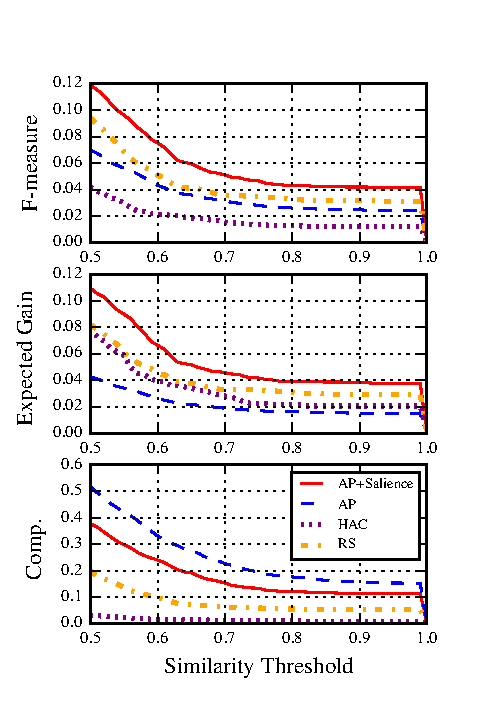
\includegraphics[]{nuggets-metrics2.eps}
\caption{Expected Gain and Comprehensiveness performance.}
\label{fig:3_aps_autots}
\end{wrapfigure}


\subsection{Model 2: LOLS}

Our next model attempts to address some of the shortcomings of the 
first. First the previous model process sentences in hourly batches.
Ideally we would process new documents as soon as possible in order 
to minimize the negative effects of latency. Second, our salience
regressors were statically trained and did not take advantage of features
like the similarity to recently selected updates and relied mostly on
tuned thresholds to account for redundancy. 

Getting around these limitations poses some severe challenges. Using
dynamic features means that naive traing will require gold reference
sentence extracts and that naively training a sentence salience model
with these will under explore the space of plausable update summaries,
meaning that in practice errors are likely to snowball over time.

Instead, we develop a clairvoyant oracle summarizer $\pi^o$ whose behavior
we want to imitate. $\pi^o$ has knowledge of what nuggets, if any, 
are present in each sentence in the document stream, and it's behavior
is quite simple: it processes each sentence in a query's relevant document 
stream and 
when it encounters a sentence with a novel nugget, it adds that sentence
to the update summary.

As we stated before, training only on a single oracle run over document stream
would be sub-optimal because the oracle is perfect and it would finish 
recovering all of the nuggets quite quickly and then do nothing for
the remainder of the stream. In practice, our learned model is likely to
make mistakes, missing the first few appearances of a nugget but hopefully
recovering them as repetition in the stream makes them more likely to be 
selected. Only following the oracle's first best pass would not help us learn
to recover from errors.

To make better use of the oracle, we adopt the locally optimal learning to
search (LOLS) algorithm \cite{lols}, one of a family of learning to search 
(L2S) algorithms. In order to formally describe the algorithm, we first 
introduce some notation. We treat the streaming summarization problem
as a markov decision process. At each timestep $t$ we observe a state
$s_t \in \mathcal{S}$ and $t$-th sentence $x_t \in \mathcal{X}$ from the 
document stream.
A policy $\pi : \mathcal{S} \times \mathcal{X} \rightarrow \{0, 1\}$
maps a state-sentence tuple to an action $a \in \mathcal{A} =\{0,1\}$
where $a=1$ indicates we extract the sentence and $a=0$ indicates we skip
the current sentence. The transition function 
$d : \mathcal{S} \times \mathcal{X} \times \mathcal{A} \rightarrow \mathcal{S}$
deterministically maps state-sentence-action tuples to the next state. 
In practice the state contains set of sentences previously extracted and
other rolling statistics from previously observed sentences in the stream.
Our training objective is to minimize the expected costs of each action:
\[ \mathcal{L}(\pi) = \mathbb{E}_{s,x \sim \pi} \left[ c\left(\pi(s,x), s, x\right) \right] \]
where $c :\mathcal{A} \times \mathcal{S} \times \mathcal{X} \rightarrow \mathcal{A}$ is the cost of taking a given action in a particular state-sentence
observation.

~\\

~\\

In the LOLS training regime, there are two phases: the 
\emph{roll-in} and the \emph{roll-out}. The roll-in phase 

at each timestep 
we alternate between using the oracle $pi^o$ or our current learned policy
$\hat{\pi}$ to run multiple time steps into the future and get a cost for 
a hypothetical summary we would have created in the case where we extracted the 
current sentence or skipped it. We collect these scores for each decision
and update a regression model to accuractely predict the cost of each action
given the current sentence and update summary/stream state.





\subsubsection{Data}
We ran 

\subsubsection{Oracle Policy and Loss Function}

We use a greedy oracle that selects sentences that contain novel
nuggets. This oracle will achieve an optimal Comprehensiveness score, i.e.
it will obtain every possible novel nugget in the roll-out phase.
However, it will not always achieve the maximum possible Expected Gain.
For example, consider the sequence of sentences $s_1, s_2, s_3$, where
nugget $n_1 \in s_1$, $n_2 \in s_2$, and $n_1,n_2 \in s_3$. The greedy oracle,
proceeding sequentially would select sentences $s_1$ and $s_2$, and skip
$s_3$, achieving an Expected Gain of $\frac{|\{n_1, n_2\}|}{|\{s_1, s_2 \}|} = \frac{2}{2} = 1$. The maximum achievable Expected Gain is obtained by skipping
the first two sentences and selecting sentence $s_3$ yielding $\frac{|\{n_1, n_2\}|}{|\{s_3 \}|} = \frac{2}{1} = 2$. In practice we are far from matching
the greedy oracle and so it suffices for now as an aspirational target.



We used the complement of Dice coefficient as the loss function.



\subsubsection{Experiments }

In our results, we refer to our learn-to-search approach as LS.
We compare to a lead sentence baseline that takes the first sentence
of every document as an update if it's maximum cosine similarity to any 
previous update was below a threshold. We refer to this method as COS.

We also compare our 








suboptimal in that it will achieve a perfect
Comprehensiveness 























